% Options for packages loaded elsewhere
% Options for packages loaded elsewhere
\PassOptionsToPackage{unicode}{hyperref}
\PassOptionsToPackage{hyphens}{url}
%
\documentclass[
  ignorenonframetext,
]{beamer}
\newif\ifbibliography
\usepackage{pgfpages}
\setbeamertemplate{caption}[numbered]
\setbeamertemplate{caption label separator}{: }
\setbeamercolor{caption name}{fg=normal text.fg}
\beamertemplatenavigationsymbolsempty
% remove section numbering
\setbeamertemplate{part page}{
  \centering
  \begin{beamercolorbox}[sep=16pt,center]{part title}
    \usebeamerfont{part title}\insertpart\par
  \end{beamercolorbox}
}
\setbeamertemplate{section page}{
  \centering
  \begin{beamercolorbox}[sep=12pt,center]{section title}
    \usebeamerfont{section title}\insertsection\par
  \end{beamercolorbox}
}
\setbeamertemplate{subsection page}{
  \centering
  \begin{beamercolorbox}[sep=8pt,center]{subsection title}
    \usebeamerfont{subsection title}\insertsubsection\par
  \end{beamercolorbox}
}
% Prevent slide breaks in the middle of a paragraph
\widowpenalties 1 10000
\raggedbottom
\AtBeginPart{
  \frame{\partpage}
}
\AtBeginSection{
  \ifbibliography
  \else
    \frame{\sectionpage}
  \fi
}
\AtBeginSubsection{
  \frame{\subsectionpage}
}
\usepackage{iftex}
\ifPDFTeX
  \usepackage[T1]{fontenc}
  \usepackage[utf8]{inputenc}
  \usepackage{textcomp} % provide euro and other symbols
\else % if luatex or xetex
  \usepackage{unicode-math} % this also loads fontspec
  \defaultfontfeatures{Scale=MatchLowercase}
  \defaultfontfeatures[\rmfamily]{Ligatures=TeX,Scale=1}
\fi
\usepackage{lmodern}

\ifPDFTeX\else
  % xetex/luatex font selection
\fi
% Use upquote if available, for straight quotes in verbatim environments
\IfFileExists{upquote.sty}{\usepackage{upquote}}{}
\IfFileExists{microtype.sty}{% use microtype if available
  \usepackage[]{microtype}
  \UseMicrotypeSet[protrusion]{basicmath} % disable protrusion for tt fonts
}{}
\makeatletter
\@ifundefined{KOMAClassName}{% if non-KOMA class
  \IfFileExists{parskip.sty}{%
    \usepackage{parskip}
  }{% else
    \setlength{\parindent}{0pt}
    \setlength{\parskip}{6pt plus 2pt minus 1pt}}
}{% if KOMA class
  \KOMAoptions{parskip=half}}
\makeatother

\usepackage{color}
\usepackage{fancyvrb}
\newcommand{\VerbBar}{|}
\newcommand{\VERB}{\Verb[commandchars=\\\{\}]}
\DefineVerbatimEnvironment{Highlighting}{Verbatim}{commandchars=\\\{\}}
% Add ',fontsize=\small' for more characters per line
\newenvironment{Shaded}{}{}
\newcommand{\AlertTok}[1]{\textcolor[rgb]{1.00,0.00,0.00}{\textbf{#1}}}
\newcommand{\AnnotationTok}[1]{\textcolor[rgb]{0.38,0.63,0.69}{\textbf{\textit{#1}}}}
\newcommand{\AttributeTok}[1]{\textcolor[rgb]{0.49,0.56,0.16}{#1}}
\newcommand{\BaseNTok}[1]{\textcolor[rgb]{0.25,0.63,0.44}{#1}}
\newcommand{\BuiltInTok}[1]{\textcolor[rgb]{0.00,0.50,0.00}{#1}}
\newcommand{\CharTok}[1]{\textcolor[rgb]{0.25,0.44,0.63}{#1}}
\newcommand{\CommentTok}[1]{\textcolor[rgb]{0.38,0.63,0.69}{\textit{#1}}}
\newcommand{\CommentVarTok}[1]{\textcolor[rgb]{0.38,0.63,0.69}{\textbf{\textit{#1}}}}
\newcommand{\ConstantTok}[1]{\textcolor[rgb]{0.53,0.00,0.00}{#1}}
\newcommand{\ControlFlowTok}[1]{\textcolor[rgb]{0.00,0.44,0.13}{\textbf{#1}}}
\newcommand{\DataTypeTok}[1]{\textcolor[rgb]{0.56,0.13,0.00}{#1}}
\newcommand{\DecValTok}[1]{\textcolor[rgb]{0.25,0.63,0.44}{#1}}
\newcommand{\DocumentationTok}[1]{\textcolor[rgb]{0.73,0.13,0.13}{\textit{#1}}}
\newcommand{\ErrorTok}[1]{\textcolor[rgb]{1.00,0.00,0.00}{\textbf{#1}}}
\newcommand{\ExtensionTok}[1]{#1}
\newcommand{\FloatTok}[1]{\textcolor[rgb]{0.25,0.63,0.44}{#1}}
\newcommand{\FunctionTok}[1]{\textcolor[rgb]{0.02,0.16,0.49}{#1}}
\newcommand{\ImportTok}[1]{\textcolor[rgb]{0.00,0.50,0.00}{\textbf{#1}}}
\newcommand{\InformationTok}[1]{\textcolor[rgb]{0.38,0.63,0.69}{\textbf{\textit{#1}}}}
\newcommand{\KeywordTok}[1]{\textcolor[rgb]{0.00,0.44,0.13}{\textbf{#1}}}
\newcommand{\NormalTok}[1]{#1}
\newcommand{\OperatorTok}[1]{\textcolor[rgb]{0.40,0.40,0.40}{#1}}
\newcommand{\OtherTok}[1]{\textcolor[rgb]{0.00,0.44,0.13}{#1}}
\newcommand{\PreprocessorTok}[1]{\textcolor[rgb]{0.74,0.48,0.00}{#1}}
\newcommand{\RegionMarkerTok}[1]{#1}
\newcommand{\SpecialCharTok}[1]{\textcolor[rgb]{0.25,0.44,0.63}{#1}}
\newcommand{\SpecialStringTok}[1]{\textcolor[rgb]{0.73,0.40,0.53}{#1}}
\newcommand{\StringTok}[1]{\textcolor[rgb]{0.25,0.44,0.63}{#1}}
\newcommand{\VariableTok}[1]{\textcolor[rgb]{0.10,0.09,0.49}{#1}}
\newcommand{\VerbatimStringTok}[1]{\textcolor[rgb]{0.25,0.44,0.63}{#1}}
\newcommand{\WarningTok}[1]{\textcolor[rgb]{0.38,0.63,0.69}{\textbf{\textit{#1}}}}

\usepackage{longtable,booktabs,array}
\usepackage{calc} % for calculating minipage widths
\usepackage{caption}
% Make caption package work with longtable
\makeatletter
\def\fnum@table{\tablename~\thetable}
\makeatother
\usepackage{graphicx}
\makeatletter
\newsavebox\pandoc@box
\newcommand*\pandocbounded[1]{% scales image to fit in text height/width
  \sbox\pandoc@box{#1}%
  \Gscale@div\@tempa{\textheight}{\dimexpr\ht\pandoc@box+\dp\pandoc@box\relax}%
  \Gscale@div\@tempb{\linewidth}{\wd\pandoc@box}%
  \ifdim\@tempb\p@<\@tempa\p@\let\@tempa\@tempb\fi% select the smaller of both
  \ifdim\@tempa\p@<\p@\scalebox{\@tempa}{\usebox\pandoc@box}%
  \else\usebox{\pandoc@box}%
  \fi%
}
% Set default figure placement to htbp
\def\fps@figure{htbp}
\makeatother


% definitions for citeproc citations
\NewDocumentCommand\citeproctext{}{}
\NewDocumentCommand\citeproc{mm}{%
  \begingroup\def\citeproctext{#2}\cite{#1}\endgroup}
\makeatletter
 % allow citations to break across lines
 \let\@cite@ofmt\@firstofone
 % avoid brackets around text for \cite:
 \def\@biblabel#1{}
 \def\@cite#1#2{{#1\if@tempswa , #2\fi}}
\makeatother
\newlength{\cslhangindent}
\setlength{\cslhangindent}{1.5em}
\newlength{\csllabelwidth}
\setlength{\csllabelwidth}{3em}
\newenvironment{CSLReferences}[2] % #1 hanging-indent, #2 entry-spacing
 {\begin{list}{}{%
  \setlength{\itemindent}{0pt}
  \setlength{\leftmargin}{0pt}
  \setlength{\parsep}{0pt}
  % turn on hanging indent if param 1 is 1
  \ifodd #1
   \setlength{\leftmargin}{\cslhangindent}
   \setlength{\itemindent}{-1\cslhangindent}
  \fi
  % set entry spacing
  \setlength{\itemsep}{#2\baselineskip}}}
 {\end{list}}
\usepackage{calc}
\newcommand{\CSLBlock}[1]{\hfill\break\parbox[t]{\linewidth}{\strut\ignorespaces#1\strut}}
\newcommand{\CSLLeftMargin}[1]{\parbox[t]{\csllabelwidth}{\strut#1\strut}}
\newcommand{\CSLRightInline}[1]{\parbox[t]{\linewidth - \csllabelwidth}{\strut#1\strut}}
\newcommand{\CSLIndent}[1]{\hspace{\cslhangindent}#1}



\setlength{\emergencystretch}{3em} % prevent overfull lines

\providecommand{\tightlist}{%
  \setlength{\itemsep}{0pt}\setlength{\parskip}{0pt}}



 


\usepackage{booktabs}
\usepackage{caption}
\usepackage{longtable}
\usepackage{colortbl}
\usepackage{array}
\usepackage{anyfontsize}
\usepackage{multirow}
% ======================= CONFIGURAÇÕES DE ESTILO ===========================
\definecolor{UFPELBlue}{RGB}{20, 49, 129}

% Cores e fonte
\setbeamercolor{headline}{bg=UFPELBlue}
\setbeamercolor{frametitle}{bg=white, fg=UFPELBlue}
\setbeamercolor{title}{fg=UFPELBlue}
\usefonttheme{default}

% Pacotes necessários
\usepackage[absolute,overlay]{textpos}
\usepackage{setspace}
\usepackage{array}
\usepackage{etoolbox}
\usepackage{graphicx}

% ======================= TEMPLATE DA PÁGINA DE TÍTULO ===========================

\defbeamertemplate*{title page}{custom-title-page}{
  \vbox to \textheight{
    % Logo IFM
    \begin{textblock*}{\textwidth}(0.2cm, 0.4cm)
      
\includegraphics[height=1cm]{logo_ifm.png}
    \end{textblock*}

    % Instituto
    \begin{textblock*}{\textwidth}(1cm, 0.5cm)
      {\usebeamerfont{institute}\tiny
      \setlength{\baselineskip}{1.5pt}
      \centering
      \renewcommand{\arraystretch}{0.2}
      \begin{tabular}{c}
        \insertinstitute
      \end{tabular}
      \par}
    \end{textblock*}

    \vfill
 % Define comando para substituir \and por \\ para autores no título
\makeatletter
\def\authorswithnewline{\def\and{\\}\insertauthor}
\makeatother


    \begin{center}
      % Título
      {\usebeamerfont{title}\usebeamercolor[fg]{title}\textbf{\inserttitle}\par}
      \vskip0.8cm
      
     

      % Autores um embaixo do outro (FORÇA)
  {\usebeamerfont{author}\usebeamercolor[fg]{author}
  \tiny
    % LISTE OS AUTORES AQUI, UM POR UM, COM \\ NO FINAL DE CADA UM
    ANA RITA DE ASSUMPÇÃO MAZZINI \\
    GISELDA MARIA PEREIRA \\
    POLLYANE VIEIRA DA SILVA \\
    ISADORA MOREIRA DA LUZ REAL \\
    ANA LUIZA BARBOZA MERLIN \\
    FERNANDO NEUGEBAUER REHBEIN DA CUNHA PENEDO \\
    LUCAS DE AZEVEDO DE SOUZA
    \par
  }
      \vskip0.4cm

      % Data
      {\usebeamerfont{date}\insertdate\par}
    \end{center}

    \vfill

    % Logos inferiores
    \begin{textblock*}{\textwidth}(11.4cm, 8cm)
      
\includegraphics[height=1.2cm]{logo_ufpel_seal.png}
    \end{textblock*}

    \begin{textblock*}{\textwidth}(0.2cm, 8.4cm)
      
\includegraphics[height=0.8cm]{RStudio.png}
    \end{textblock*}
  }
}
% ======================= OUTROS AJUSTES ===========================

% Frame title centralizado
\setbeamertemplate{frametitle}{%
  \begin{center}\textbf{\insertframetitle}\end{center}
}

% Barra azul superior em todos os frames
\setbeamertemplate{headline}{%
  \leavevmode
  \hbox{%
    \begin{beamercolorbox}[wd=\paperwidth,ht=2.5ex,dp=1.5ex]{headline}
    \end{beamercolorbox}%
  }
  % Logo R no canto superior direito
  \begin{textblock*}{2cm}(0.88\paperwidth,0.4cm)
    
\includegraphics[height=1cm]{logo_r.png}
  \end{textblock*}
}

% Barra azul inferior em todos os frames
\setbeamertemplate{footline}{%
  \leavevmode
  \hbox{%
    \begin{beamercolorbox}[wd=\paperwidth,ht=2.5ex,dp=1.5ex]{headline}
    \end{beamercolorbox}%
  }
}

\makeatletter
\@ifpackageloaded{caption}{}{\usepackage{caption}}
\AtBeginDocument{%
\ifdefined\contentsname
  \renewcommand*\contentsname{Table of contents}
\else
  \newcommand\contentsname{Table of contents}
\fi
\ifdefined\listfigurename
  \renewcommand*\listfigurename{List of Figures}
\else
  \newcommand\listfigurename{List of Figures}
\fi
\ifdefined\listtablename
  \renewcommand*\listtablename{List of Tables}
\else
  \newcommand\listtablename{List of Tables}
\fi
\ifdefined\figurename
  \renewcommand*\figurename{Figure}
\else
  \newcommand\figurename{Figure}
\fi
\ifdefined\tablename
  \renewcommand*\tablename{Table}
\else
  \newcommand\tablename{Table}
\fi
}
\@ifpackageloaded{float}{}{\usepackage{float}}
\floatstyle{ruled}
\@ifundefined{c@chapter}{\newfloat{codelisting}{h}{lop}}{\newfloat{codelisting}{h}{lop}[chapter]}
\floatname{codelisting}{Listing}
\newcommand*\listoflistings{\listof{codelisting}{List of Listings}}
\makeatother
\makeatletter
\makeatother
\makeatletter
\@ifpackageloaded{caption}{}{\usepackage{caption}}
\@ifpackageloaded{subcaption}{}{\usepackage{subcaption}}
\makeatother

\usepackage{bookmark}
\IfFileExists{xurl.sty}{\usepackage{xurl}}{} % add URL line breaks if available
\urlstyle{same}
\hypersetup{
  pdftitle={Introdução ao ggplot2},
  hidelinks,
  pdfcreator={LaTeX via pandoc}}


\title{Introdução ao ggplot2}
\author{}
\date{}
\institute{UNIVERSIDADE FEDERAL DE PELOTAS \and INSTITUTO DE FÍSICA E
MATEMÁTICA -- IFM}

\begin{document}
\frame{\titlepage}


\begin{frame}[fragile]{Introdução}
\phantomsection\label{introduuxe7uxe3o}
O \texttt{ggplot2} é um pacote de código aberto para a visualização
gráfica de dados para a linguagem de programação R. Foi criada por
Hadley Wickham em 2005 (Wickham 2016), sendo uma implementação do livro
\texttt{Grammar\ Graphics} de Leland Wilkison também lançado em 2005
(Wilkinson 2011).

Ele aborda que visualização gráfica dos dados pode ser divida em
componentes semânticos, como escalas e camadas.

\begin{center}
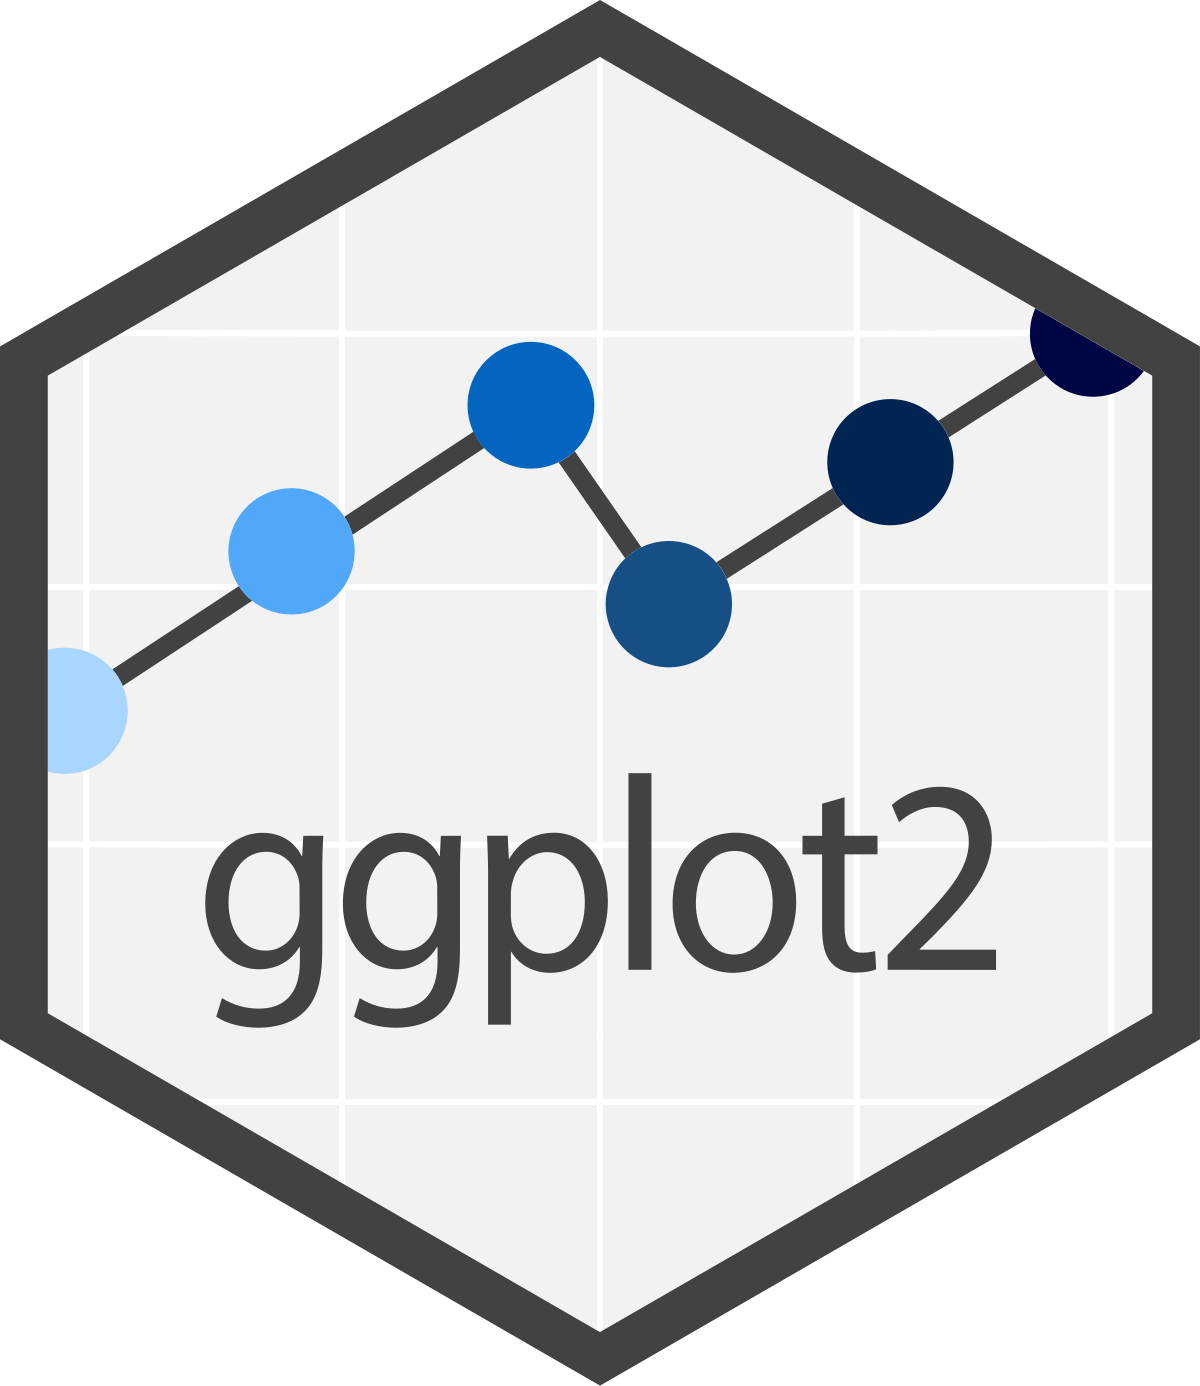
\includegraphics[width=0.2\linewidth,height=\textheight,keepaspectratio]{Ggplot2_hex_logo.svg.png}
\end{center}
\end{frame}

\begin{frame}[fragile]{Por que usar o ggplot2?}
\phantomsection\label{por-que-usar-o-ggplot2}
\begin{enumerate}
\item
  Alta costumização gráfica.
\item
  Alta diversidade de modelos de gráficos.
\item
  Integração com outros pacotes do tidyverse, como por exemplo
  \texttt{dplyr} (Wickham et al. 2023), \texttt{forcats} (Wickham 2023)
  e o \texttt{plotly} (Sievert 2020).
\item
  Criação de gráficos a partir de camadas, podendo sobrepor diferentes
  gráficos.
\end{enumerate}
\end{frame}

\begin{frame}[fragile]{Como instalar o ggplot2?}
\phantomsection\label{como-instalar-o-ggplot2}
\begin{Shaded}
\begin{Highlighting}[]
\CommentTok{\#instalando pacote ggplot2}
\FunctionTok{install.packages}\NormalTok{(}\StringTok{"ggplot2"}\NormalTok{)}

\CommentTok{\#instalando dplyr, forcats e patchwork}
\FunctionTok{install.packages}\NormalTok{(}\StringTok{"dplyr"}\NormalTok{)}
\FunctionTok{install.packages}\NormalTok{(}\StringTok{"forcats"}\NormalTok{)}
\FunctionTok{install.packages}\NormalTok{(}\StringTok{"patchwork"}\NormalTok{)}
\end{Highlighting}
\end{Shaded}
\end{frame}

\begin{frame}[fragile]
Para usar o \texttt{ggplot2} em seus scripts tem que carrega-lo

\begin{Shaded}
\begin{Highlighting}[]
\CommentTok{\#Carregando o pacote ggplot2}
\FunctionTok{library}\NormalTok{(ggplot2)}

\CommentTok{\#Carregando dplyr, forcats e patchwork}
\FunctionTok{library}\NormalTok{(dplyr)}
\FunctionTok{library}\NormalTok{(forcats)}
\FunctionTok{library}\NormalTok{(patchwork)}
\end{Highlighting}
\end{Shaded}
\end{frame}

\begin{frame}[fragile]{Banco de dados \emph{iris}}
\phantomsection\label{banco-de-dados-iris}
Para essa oficina será utilizado bancos de dados \textbf{iris}.

\textbf{iris} - é referente tamanho de pételas e sepalas de 3 espécies
do gênero \emph{Iris} do trabalho de Fisher em 1936 (\emph{Iris
setosa},\emph{Iris versicolor} e \emph{Iris virginica})

\begin{Shaded}
\begin{Highlighting}[]
\FunctionTok{data}\NormalTok{(iris)}
\end{Highlighting}
\end{Shaded}

\begin{table}
\fontsize{7.5pt}{9.0pt}\selectfont
\begin{tabular*}{\linewidth}{@{\extracolsep{\fill}}rrrrc}
\toprule
Sepal.Length & Sepal.Width & Petal.Length & Petal.Width & Species \\ 
\midrule\addlinespace[2.5pt]
5.1 & 3.5 & 1.4 & 0.2 & setosa \\ 
4.9 & 3.0 & 1.4 & 0.2 & setosa \\ 
4.7 & 3.2 & 1.3 & 0.2 & setosa \\ 
4.6 & 3.1 & 1.5 & 0.2 & setosa \\ 
\bottomrule
\end{tabular*}
\end{table}
\end{frame}

\begin{frame}[fragile]{Box-plot}
\phantomsection\label{box-plot}
\begin{Shaded}
\begin{Highlighting}[]
\NormalTok{iris}\SpecialCharTok{\%\textgreater{}\%}\FunctionTok{ggplot}\NormalTok{(}\FunctionTok{aes}\NormalTok{(}\AttributeTok{x=}\NormalTok{Species, }\AttributeTok{y=}\NormalTok{Petal.Length))}\SpecialCharTok{+}
  \FunctionTok{geom\_boxplot}\NormalTok{()}
\end{Highlighting}
\end{Shaded}
\end{frame}

\begin{frame}
\pandocbounded{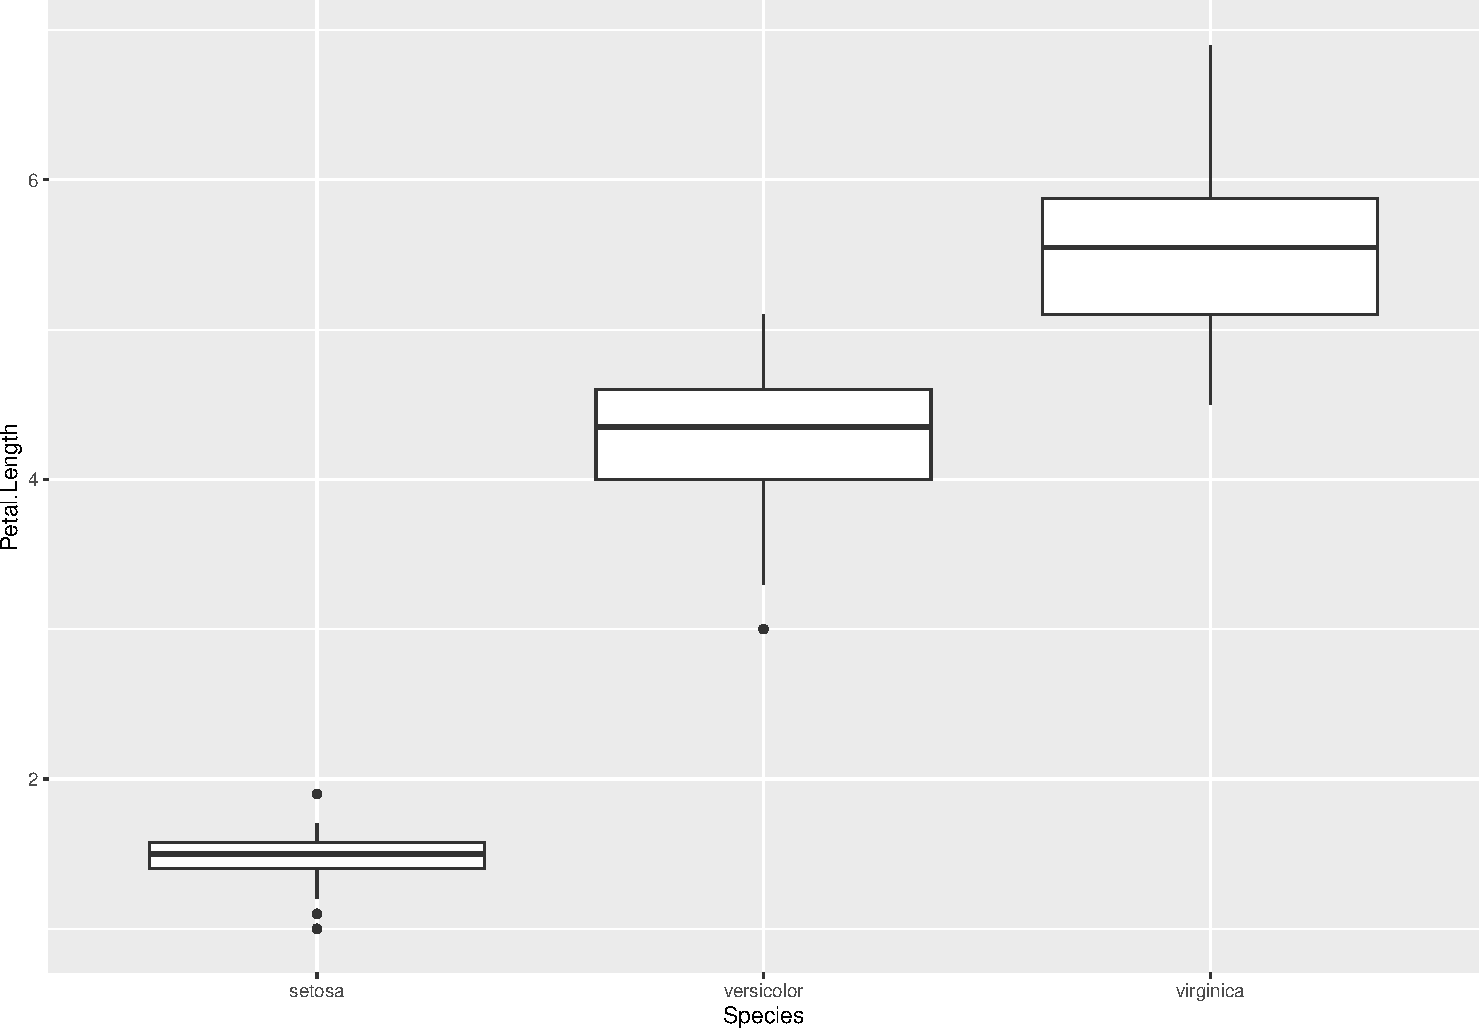
\includegraphics[keepaspectratio]{index_beamer_files/figure-beamer/Box-plot simplesx-1.pdf}}
\end{frame}

\begin{frame}[fragile]{Gráfico violino}
\phantomsection\label{gruxe1fico-violino}
\begin{Shaded}
\begin{Highlighting}[]
\FunctionTok{ggplot}\NormalTok{(iris, }\FunctionTok{aes}\NormalTok{(}\AttributeTok{x=}\NormalTok{Species,}\AttributeTok{y=}\NormalTok{Sepal.Width, }\AttributeTok{fill=}\NormalTok{Species))}\SpecialCharTok{+}
  \FunctionTok{geom\_violin}\NormalTok{()}
\end{Highlighting}
\end{Shaded}

\pandocbounded{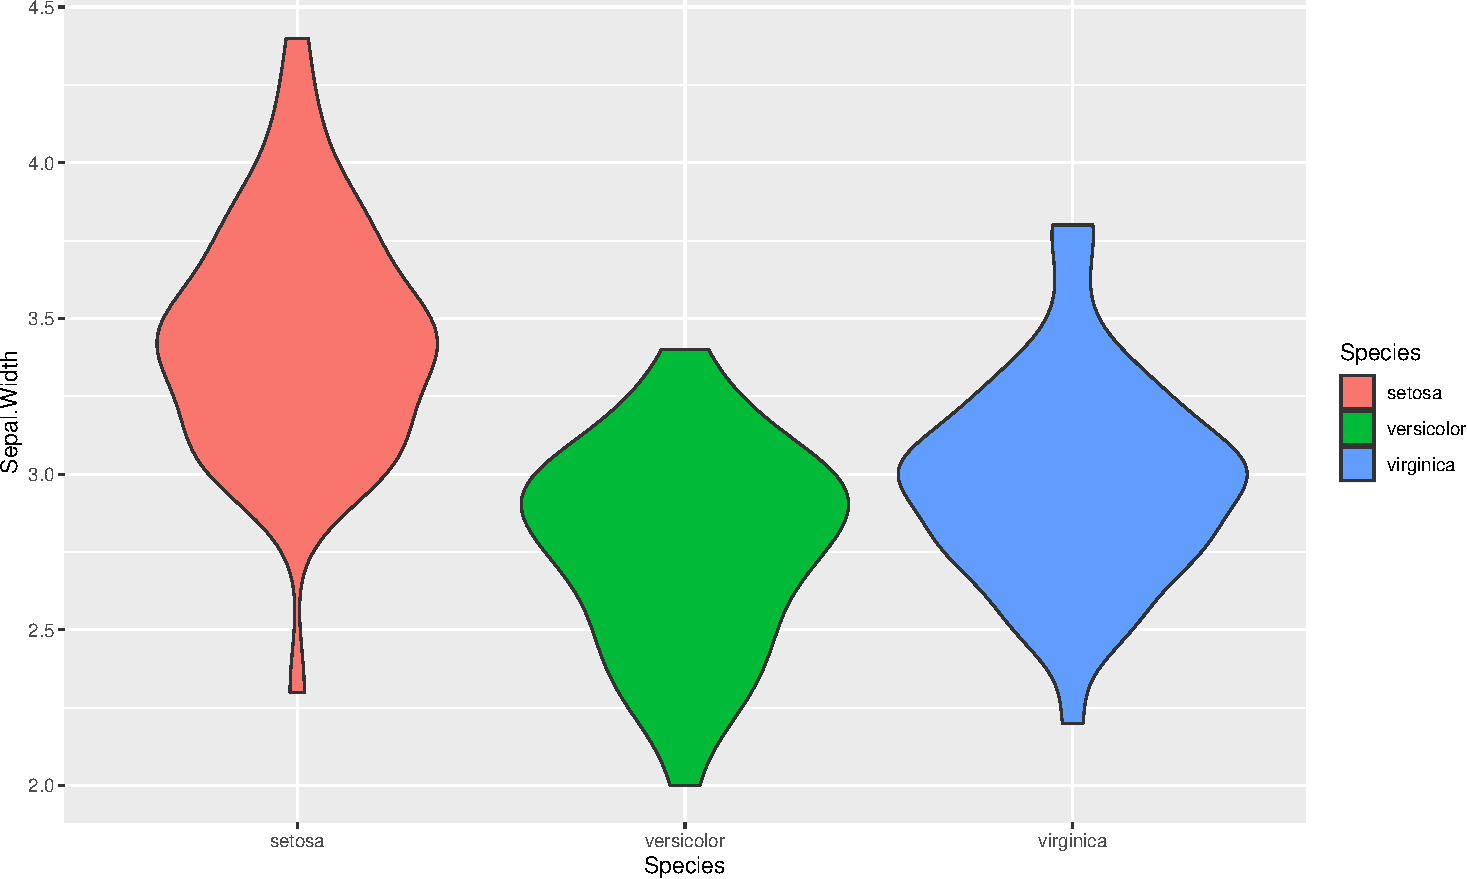
\includegraphics[keepaspectratio]{index_beamer_files/figure-beamer/violino-1.pdf}}
\end{frame}

\begin{frame}[fragile]{Histograma}
\phantomsection\label{histograma}
\begin{Shaded}
\begin{Highlighting}[]
\FunctionTok{ggplot}\NormalTok{(iris,}\FunctionTok{aes}\NormalTok{(}\AttributeTok{x=}\NormalTok{Sepal.Width))}\SpecialCharTok{+}
  \FunctionTok{geom\_histogram}\NormalTok{(}\AttributeTok{bins=}\DecValTok{10}\NormalTok{, }\AttributeTok{color=}\StringTok{"black"}\NormalTok{,}
                 \AttributeTok{fill=}\StringTok{"white"}\NormalTok{)}\SpecialCharTok{+}
  \FunctionTok{labs}\NormalTok{(}\AttributeTok{y=}\StringTok{"Frequência"}\NormalTok{, }\AttributeTok{x=}\StringTok{"Largura de Sépala"}\NormalTok{)}
\end{Highlighting}
\end{Shaded}

\pandocbounded{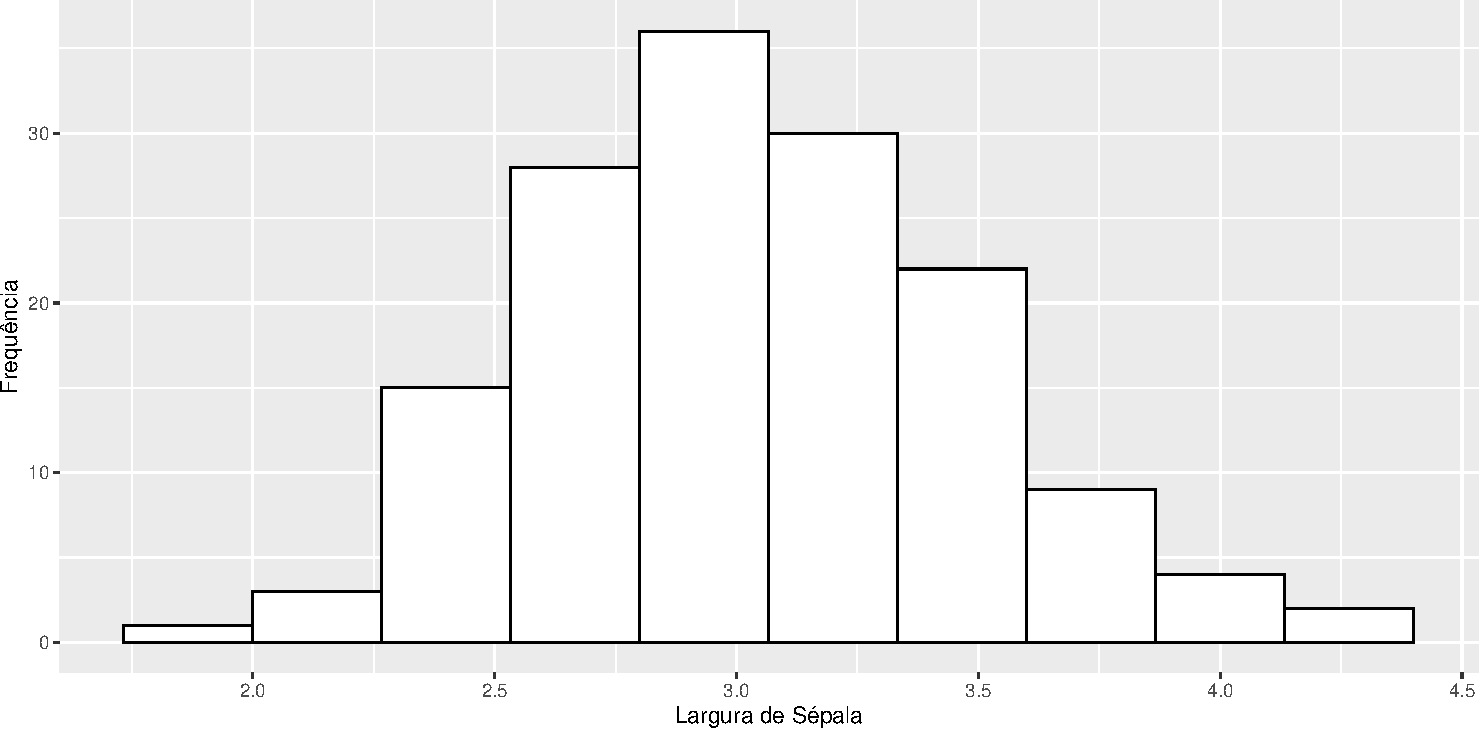
\includegraphics[keepaspectratio]{index_beamer_files/figure-beamer/histograma-1.pdf}}
\end{frame}

\begin{frame}[fragile]
\begin{Shaded}
\begin{Highlighting}[]
\FunctionTok{ggplot}\NormalTok{(iris,}\FunctionTok{aes}\NormalTok{(}\AttributeTok{x=}\NormalTok{Sepal.Width))}\SpecialCharTok{+}
  \FunctionTok{geom\_histogram}\NormalTok{(}\AttributeTok{bins=}\DecValTok{11}\NormalTok{, }\AttributeTok{color=}\StringTok{"black"}\NormalTok{,}
                 \AttributeTok{fill=}\StringTok{"white"}\NormalTok{)}\SpecialCharTok{+}
  \FunctionTok{labs}\NormalTok{(}\AttributeTok{y=}\StringTok{"Frequência"}\NormalTok{, }\AttributeTok{x=}\StringTok{"Largura de Sépala"}\NormalTok{)}\SpecialCharTok{+}
  \FunctionTok{scale\_x\_continuous}\NormalTok{(}\AttributeTok{n.breaks =} \DecValTok{11}\NormalTok{)}
\end{Highlighting}
\end{Shaded}

\pandocbounded{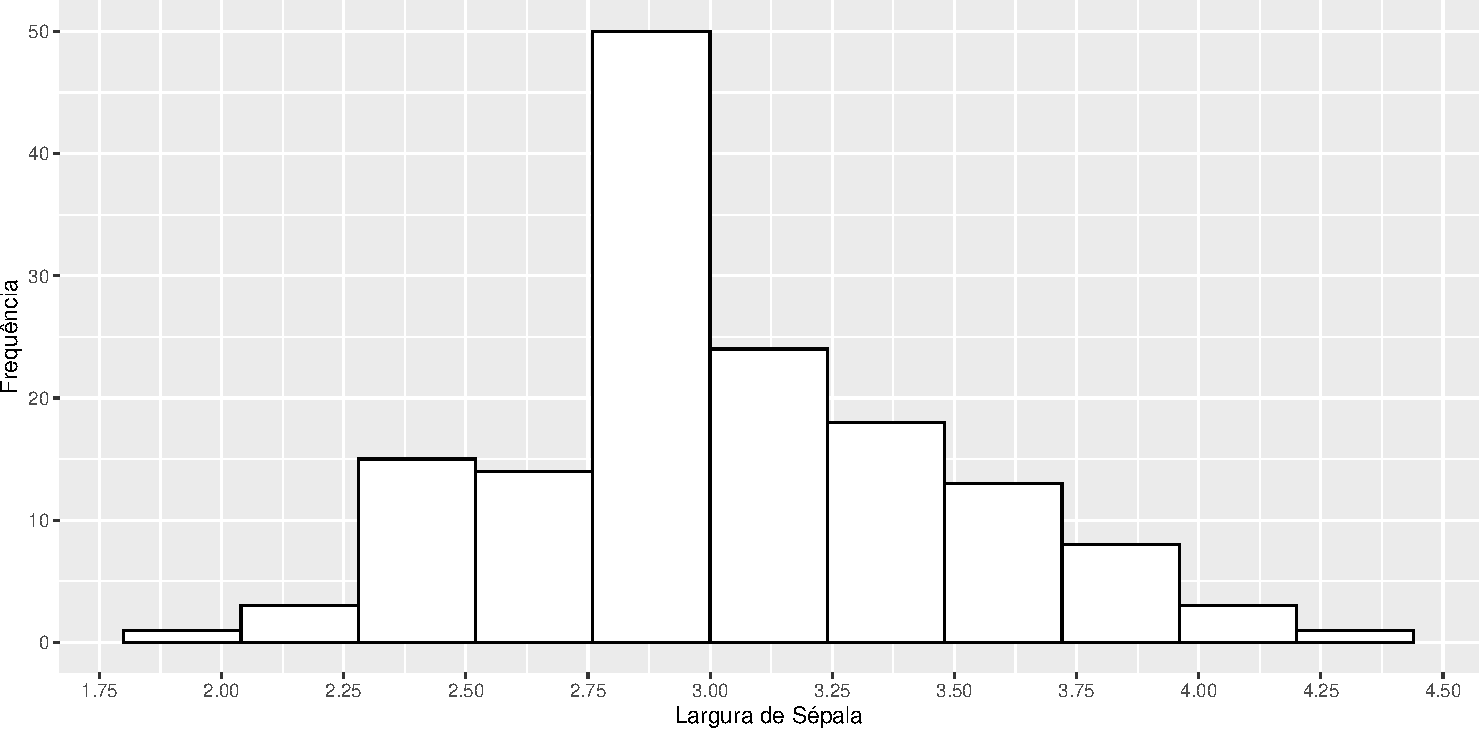
\includegraphics[keepaspectratio]{index_beamer_files/figure-beamer/unnamed-chunk-2-1.pdf}}
\end{frame}

\begin{frame}[fragile]{Polígono}
\phantomsection\label{poluxedgono}
\begin{Shaded}
\begin{Highlighting}[]
\FunctionTok{ggplot}\NormalTok{(iris,}\FunctionTok{aes}\NormalTok{(}\AttributeTok{x=}\NormalTok{Sepal.Width))}\SpecialCharTok{+}
  \FunctionTok{geom\_freqpoly}\NormalTok{(}\AttributeTok{bins=}\DecValTok{11}\NormalTok{, }\AttributeTok{color=}\StringTok{"black"}\NormalTok{)}\SpecialCharTok{+}
  \FunctionTok{labs}\NormalTok{(}\AttributeTok{y=}\StringTok{"Frequência"}\NormalTok{, }\AttributeTok{x=}\StringTok{"Largura de Sépala"}\NormalTok{)}\SpecialCharTok{+}
  \FunctionTok{scale\_x\_continuous}\NormalTok{(}\AttributeTok{n.breaks =} \DecValTok{11}\NormalTok{)}
\end{Highlighting}
\end{Shaded}

\pandocbounded{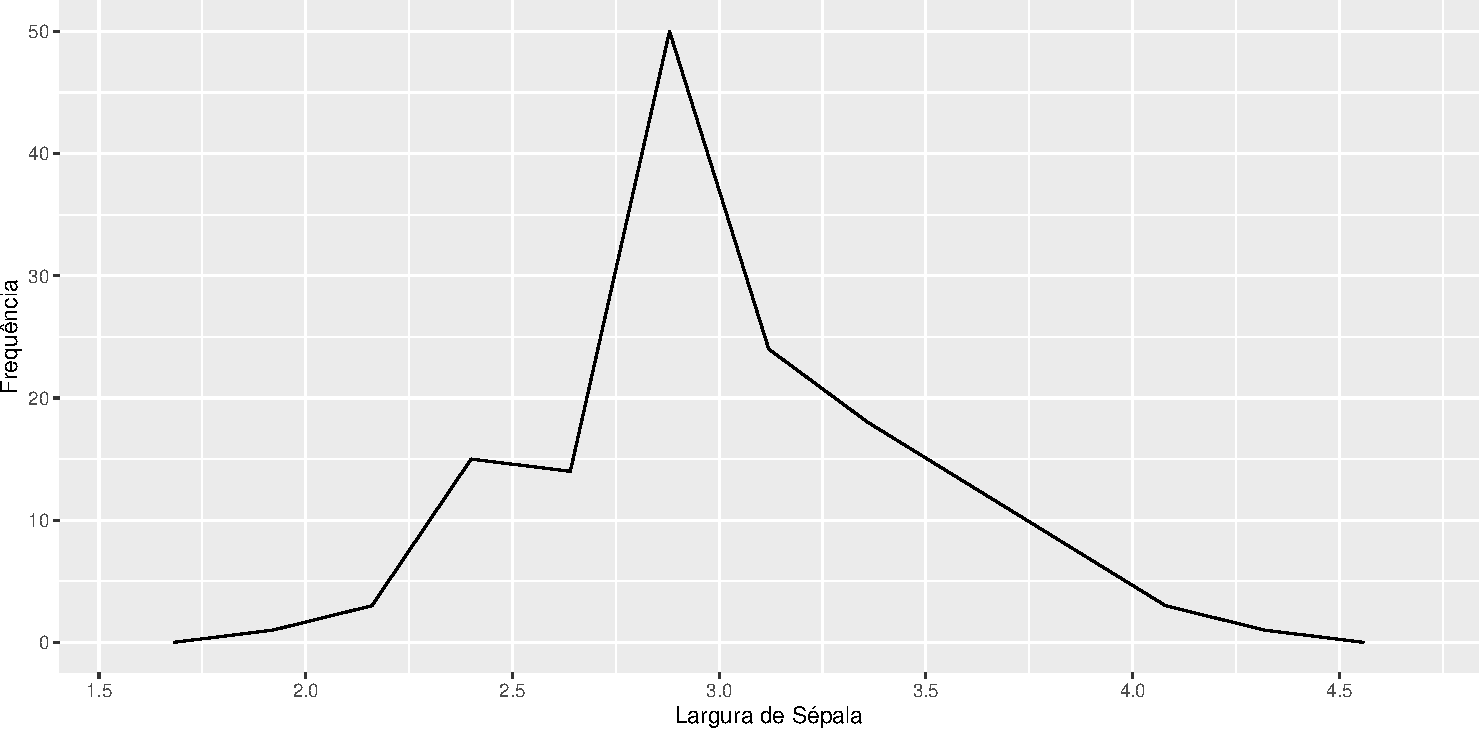
\includegraphics[keepaspectratio]{index_beamer_files/figure-beamer/histograma1-1.pdf}}
\end{frame}

\begin{frame}[fragile]
\begin{Shaded}
\begin{Highlighting}[]
\FunctionTok{ggplot}\NormalTok{(iris,}\FunctionTok{aes}\NormalTok{(}\AttributeTok{x=}\NormalTok{Sepal.Width))}\SpecialCharTok{+}
  \FunctionTok{labs}\NormalTok{(}\AttributeTok{y=}\StringTok{"Frequência"}\NormalTok{, }\AttributeTok{x=}\StringTok{"Largura de Sépala"}\NormalTok{)}\SpecialCharTok{+}
  \FunctionTok{scale\_x\_continuous}\NormalTok{(}\AttributeTok{n.breaks =} \DecValTok{11}\NormalTok{)}\SpecialCharTok{+}
  \FunctionTok{geom\_histogram}\NormalTok{(}\AttributeTok{bins=}\DecValTok{11}\NormalTok{, }\AttributeTok{color=}\StringTok{"black"}\NormalTok{,}
                 \AttributeTok{fill=}\StringTok{"white"}\NormalTok{)}\SpecialCharTok{+}
  \FunctionTok{geom\_freqpoly}\NormalTok{(}\AttributeTok{bins=}\DecValTok{11}\NormalTok{, }\AttributeTok{color=}\StringTok{"blue"}\NormalTok{)}
\end{Highlighting}
\end{Shaded}

\pandocbounded{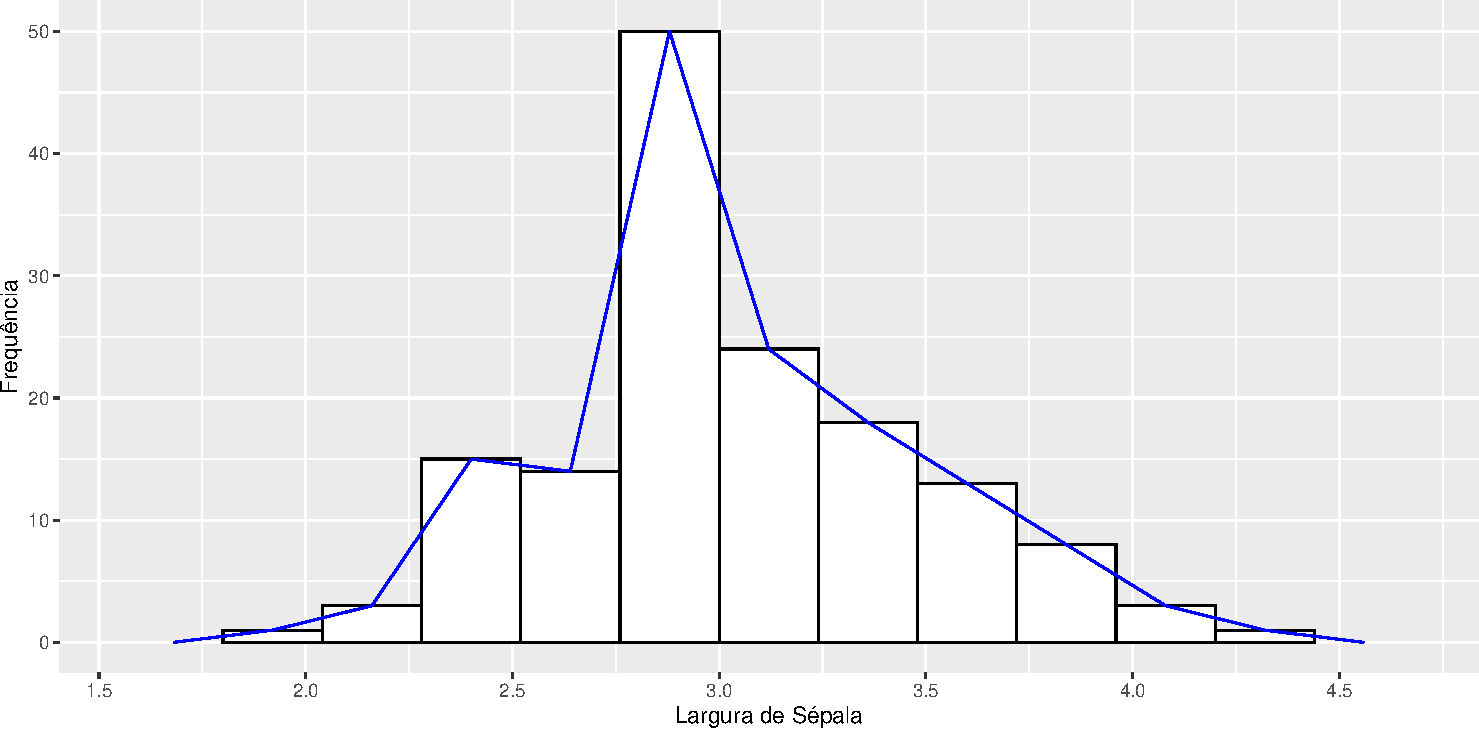
\includegraphics[keepaspectratio]{index_beamer_files/figure-beamer/unnamed-chunk-3-1.pdf}}
\end{frame}

\begin{frame}[fragile]
\begin{Shaded}
\begin{Highlighting}[]
\FunctionTok{ggplot}\NormalTok{(iris,}\FunctionTok{aes}\NormalTok{(}\AttributeTok{x=}\NormalTok{Sepal.Width))}\SpecialCharTok{+}
  \FunctionTok{labs}\NormalTok{(}\AttributeTok{y=}\StringTok{"Frequência"}\NormalTok{, }\AttributeTok{x=}\StringTok{"Largura de Sépala"}\NormalTok{)}\SpecialCharTok{+}
  \FunctionTok{scale\_x\_continuous}\NormalTok{(}\AttributeTok{n.breaks =} \DecValTok{11}\NormalTok{)}\SpecialCharTok{+}
  \FunctionTok{geom\_histogram}\NormalTok{(}\AttributeTok{bins=}\DecValTok{11}\NormalTok{, }\AttributeTok{color=}\StringTok{"black"}\NormalTok{,}
                 \AttributeTok{fill=}\StringTok{"white"}\NormalTok{)}\SpecialCharTok{+}
  \FunctionTok{geom\_freqpoly}\NormalTok{(}\AttributeTok{bins=}\DecValTok{11}\NormalTok{, }\AttributeTok{color=}\StringTok{"blue"}\NormalTok{)}\SpecialCharTok{+}
  \FunctionTok{facet\_grid}\NormalTok{(}\SpecialCharTok{\textasciitilde{}}\NormalTok{Species)}
\end{Highlighting}
\end{Shaded}

\pandocbounded{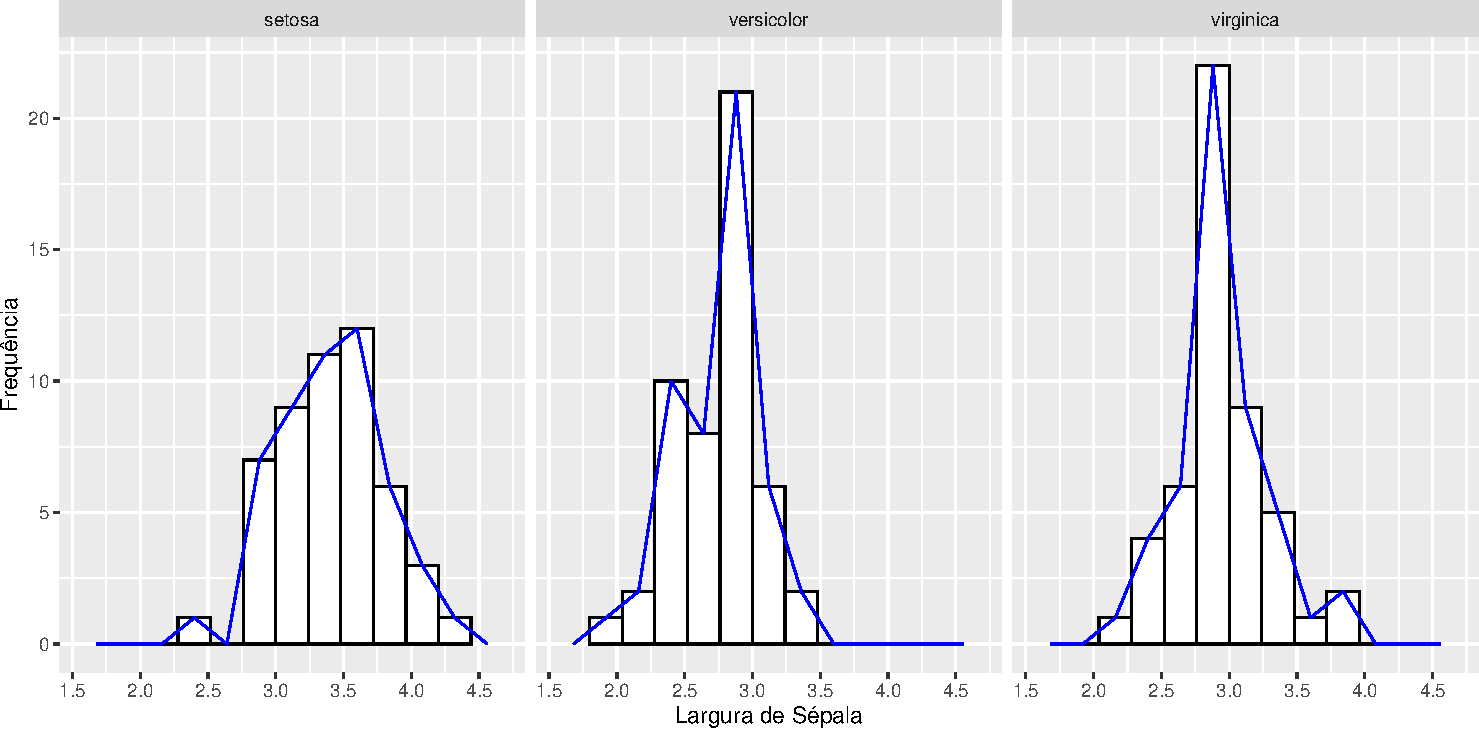
\includegraphics[keepaspectratio]{index_beamer_files/figure-beamer/unnamed-chunk-4-1.pdf}}
\end{frame}

\begin{frame}[fragile]
\begin{Shaded}
\begin{Highlighting}[]
\FunctionTok{ggplot}\NormalTok{(iris,}\FunctionTok{aes}\NormalTok{(}\AttributeTok{x=}\NormalTok{Sepal.Width))}\SpecialCharTok{+}
  \FunctionTok{labs}\NormalTok{(}\AttributeTok{y=}\StringTok{"Frequência"}\NormalTok{, }\AttributeTok{x=}\StringTok{"Largura de Sépala"}\NormalTok{)}\SpecialCharTok{+}
  \FunctionTok{scale\_x\_continuous}\NormalTok{(}\AttributeTok{n.breaks =} \DecValTok{11}\NormalTok{)}\SpecialCharTok{+}
  \FunctionTok{geom\_histogram}\NormalTok{(}\AttributeTok{bins=}\DecValTok{11}\NormalTok{, }\AttributeTok{color=}\StringTok{"black"}\NormalTok{,}
                 \AttributeTok{fill=}\StringTok{"white"}\NormalTok{)}\SpecialCharTok{+}
  \FunctionTok{geom\_freqpoly}\NormalTok{(}\AttributeTok{bins=}\DecValTok{11}\NormalTok{, }\AttributeTok{color=}\StringTok{"blue"}\NormalTok{)}\SpecialCharTok{+}
  \FunctionTok{facet\_grid}\NormalTok{(Species}\SpecialCharTok{\textasciitilde{}}\NormalTok{.)}
\end{Highlighting}
\end{Shaded}

\pandocbounded{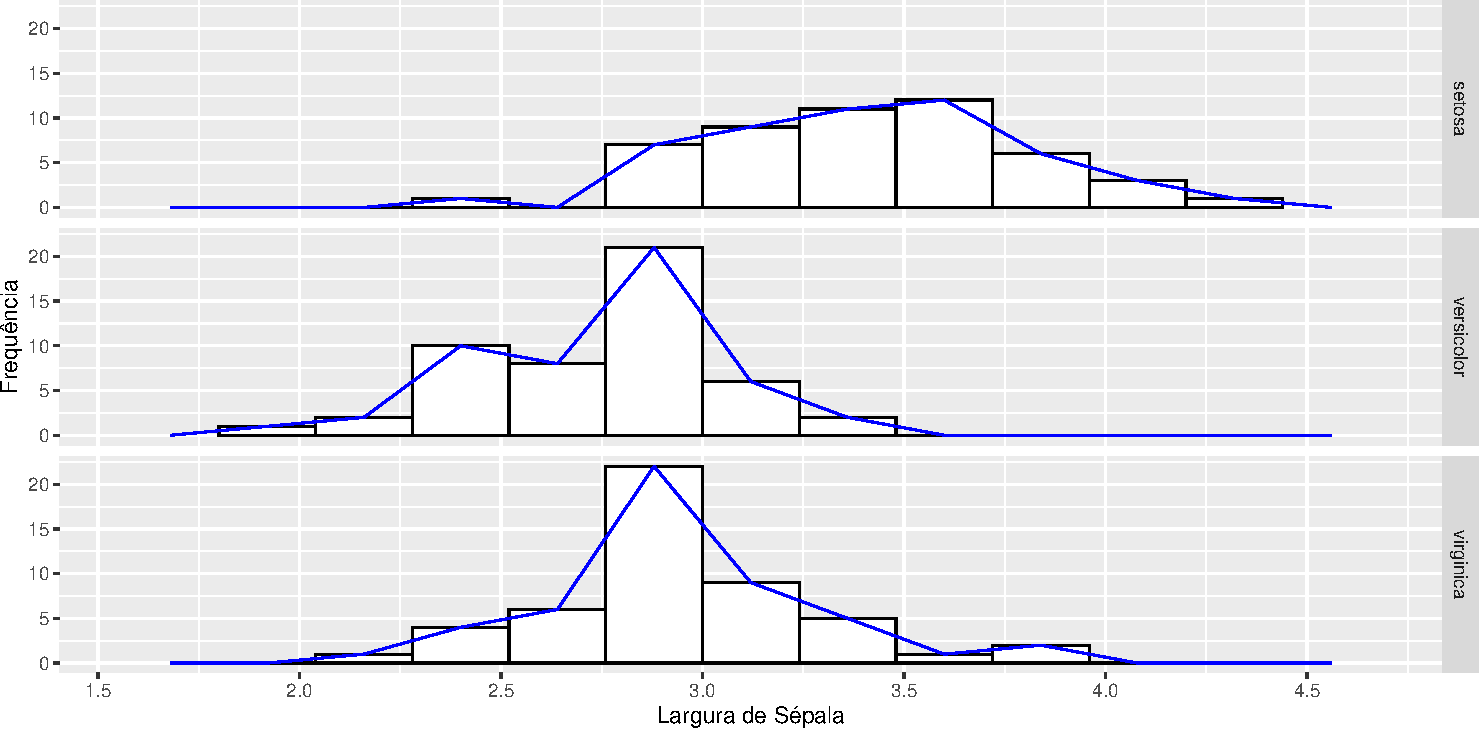
\includegraphics[keepaspectratio]{index_beamer_files/figure-beamer/unnamed-chunk-5-1.pdf}}
\end{frame}

\begin{frame}[fragile]{Gráfico de densidade}
\phantomsection\label{gruxe1fico-de-densidade}
\begin{Shaded}
\begin{Highlighting}[]
\FunctionTok{ggplot}\NormalTok{(iris,}\FunctionTok{aes}\NormalTok{(}\AttributeTok{x=}\NormalTok{Sepal.Width))}\SpecialCharTok{+}
  \FunctionTok{geom\_density}\NormalTok{(}\AttributeTok{color=}\StringTok{"black"}\NormalTok{, }\AttributeTok{fill=}\StringTok{"white"}\NormalTok{)}\SpecialCharTok{+}
  \FunctionTok{labs}\NormalTok{(}\AttributeTok{y=}\StringTok{"Frequência"}\NormalTok{, }\AttributeTok{x=}\StringTok{"Largura de Sépala"}\NormalTok{)}
\end{Highlighting}
\end{Shaded}

\pandocbounded{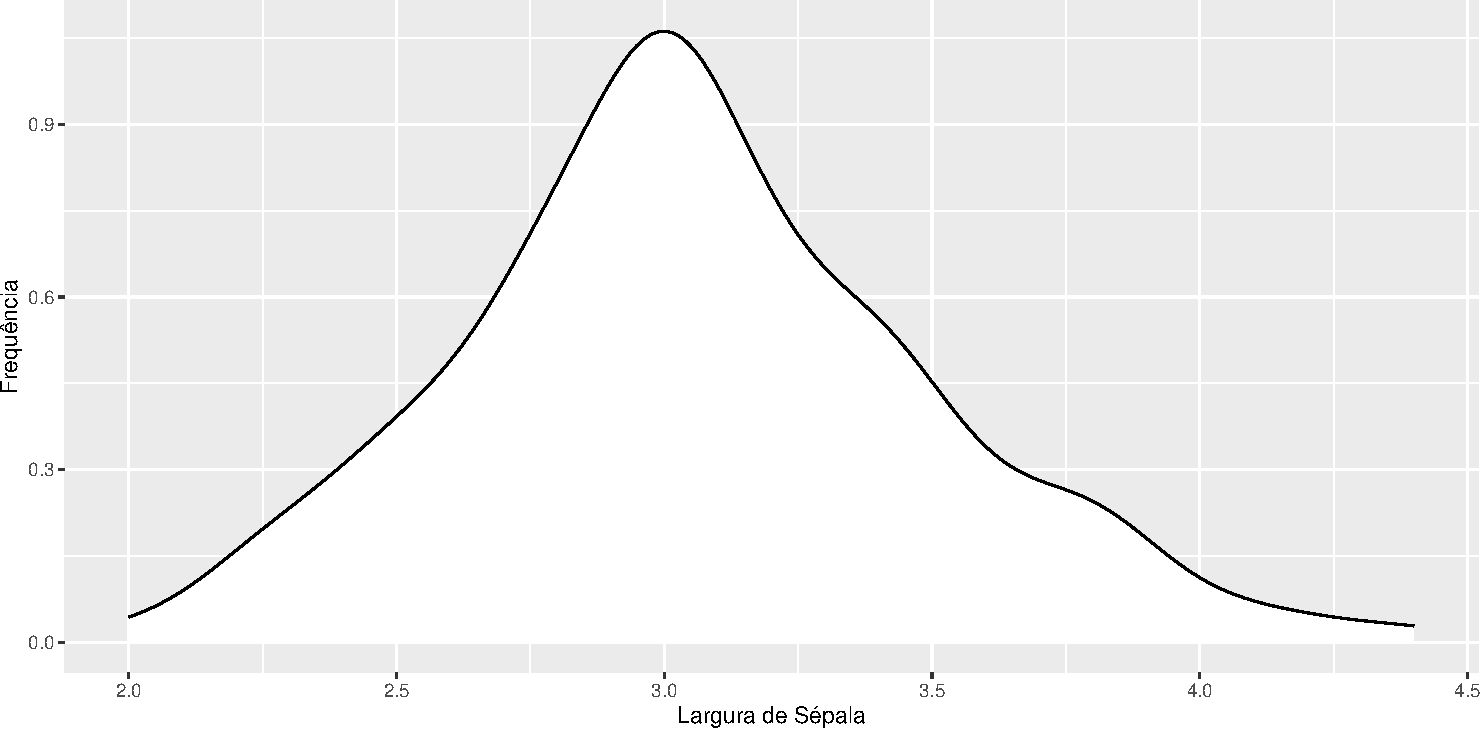
\includegraphics[keepaspectratio]{index_beamer_files/figure-beamer/unnamed-chunk-6-1.pdf}}
\end{frame}

\begin{frame}[fragile]{Gráfico de barras de frequência}
\phantomsection\label{gruxe1fico-de-barras-de-frequuxeancia}
\begin{Shaded}
\begin{Highlighting}[]
\NormalTok{iris}\SpecialCharTok{\%\textgreater{}\%}\FunctionTok{ggplot}\NormalTok{(}\FunctionTok{aes}\NormalTok{(}\AttributeTok{x=}\NormalTok{Species))}\SpecialCharTok{+}
  \FunctionTok{geom\_bar}\NormalTok{()}
\end{Highlighting}
\end{Shaded}

\pandocbounded{\includegraphics[keepaspectratio]{index_beamer_files/figure-beamer/Frequência-1.pdf}}
\end{frame}

\begin{frame}[fragile]
\begin{Shaded}
\begin{Highlighting}[]
\NormalTok{iris}\SpecialCharTok{\%\textgreater{}\%}\FunctionTok{group\_by}\NormalTok{(Species)}\SpecialCharTok{\%\textgreater{}\%}
  \FunctionTok{summarise}\NormalTok{(}\AttributeTok{count=}\FunctionTok{n}\NormalTok{())}\SpecialCharTok{\%\textgreater{}\%}
  \FunctionTok{ggplot}\NormalTok{(}\FunctionTok{aes}\NormalTok{(}\AttributeTok{x=}\NormalTok{Species, }\AttributeTok{fill=}\NormalTok{Species, }\AttributeTok{y=}\NormalTok{count))}\SpecialCharTok{+}
  \FunctionTok{geom\_col}\NormalTok{(}\AttributeTok{color=}\StringTok{"black"}\NormalTok{)}
\end{Highlighting}
\end{Shaded}

\pandocbounded{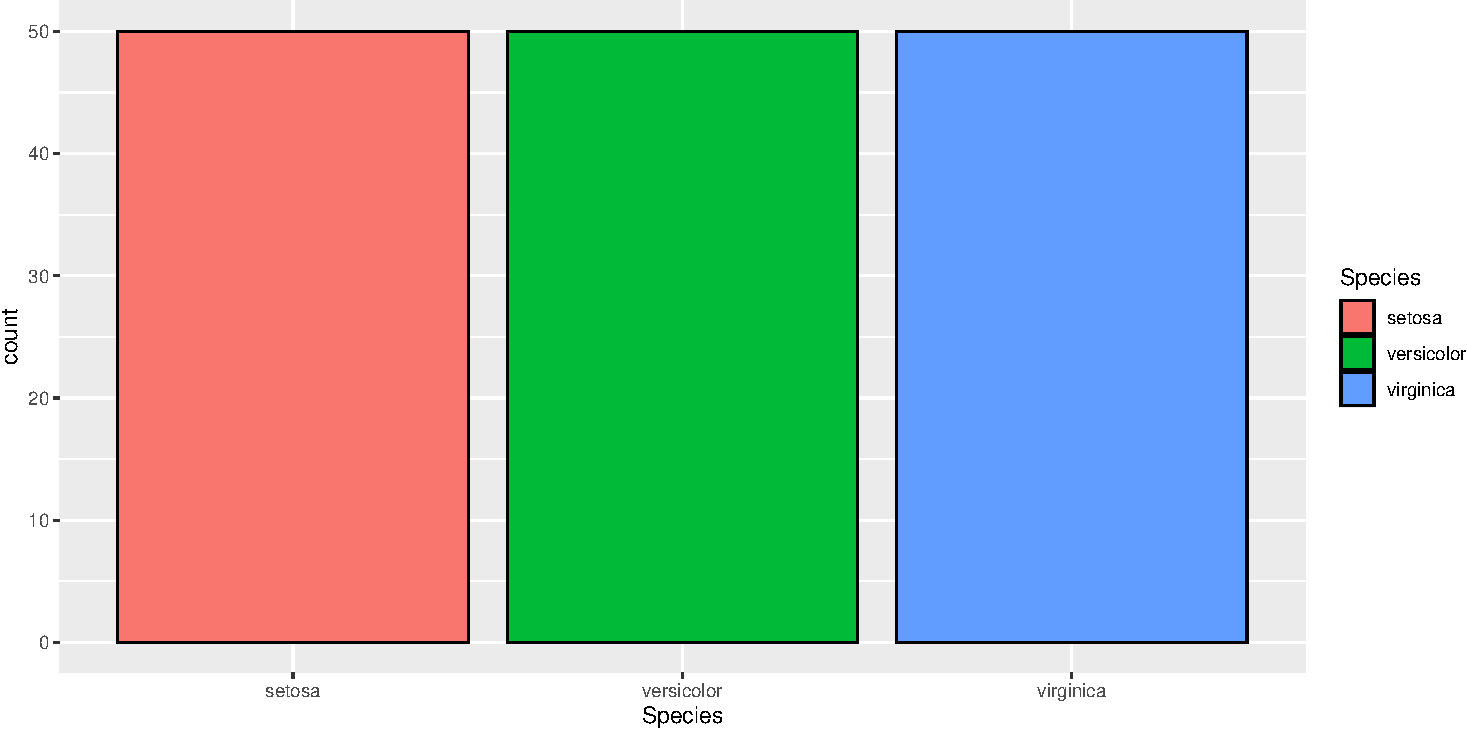
\includegraphics[keepaspectratio]{index_beamer_files/figure-beamer/unnamed-chunk-7-1.pdf}}
\end{frame}

\begin{frame}[fragile]{Gráfico de pizza}
\phantomsection\label{gruxe1fico-de-pizza}
\begin{Shaded}
\begin{Highlighting}[]
\NormalTok{iris}\SpecialCharTok{\%\textgreater{}\%}\FunctionTok{group\_by}\NormalTok{(Species)}\SpecialCharTok{\%\textgreater{}\%}
  \FunctionTok{summarise}\NormalTok{(}\AttributeTok{count=}\FunctionTok{n}\NormalTok{()}\SpecialCharTok{/}\DecValTok{150}\SpecialCharTok{*}\DecValTok{100}\NormalTok{)}\SpecialCharTok{\%\textgreater{}\%}
  \FunctionTok{ggplot}\NormalTok{(}\FunctionTok{aes}\NormalTok{(}\AttributeTok{x=}\StringTok{" "}\NormalTok{, }\AttributeTok{fill=}\NormalTok{Species, }\AttributeTok{y=}\NormalTok{count))}\SpecialCharTok{+}
  \FunctionTok{geom\_col}\NormalTok{(}\AttributeTok{color=}\StringTok{"black"}\NormalTok{)}\SpecialCharTok{+}
  \FunctionTok{coord\_polar}\NormalTok{(}\AttributeTok{theta=}\StringTok{"y"}\NormalTok{)}\SpecialCharTok{+}
  \FunctionTok{theme\_void}\NormalTok{()}
\end{Highlighting}
\end{Shaded}

\pandocbounded{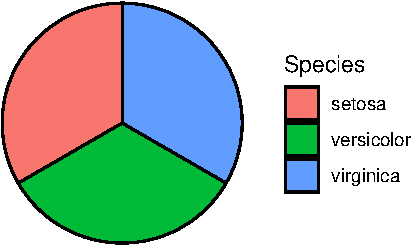
\includegraphics[keepaspectratio]{index_beamer_files/figure-beamer/unnamed-chunk-8-1.pdf}}
\end{frame}

\begin{frame}[fragile]
\begin{Shaded}
\begin{Highlighting}[]
\NormalTok{iris}\SpecialCharTok{\%\textgreater{}\%}\FunctionTok{group\_by}\NormalTok{(Species)}\SpecialCharTok{\%\textgreater{}\%}
  \FunctionTok{summarise}\NormalTok{(}\AttributeTok{count=}\FunctionTok{round}\NormalTok{(}\FunctionTok{n}\NormalTok{()}\SpecialCharTok{/}\DecValTok{150}\SpecialCharTok{*}\DecValTok{100}\NormalTok{, }\DecValTok{2}\NormalTok{))}\SpecialCharTok{\%\textgreater{}\%}
  \FunctionTok{ggplot}\NormalTok{(}\FunctionTok{aes}\NormalTok{(}\AttributeTok{x=}\StringTok{" "}\NormalTok{, }\AttributeTok{fill=}\NormalTok{Species, }\AttributeTok{y=}\NormalTok{count))}\SpecialCharTok{+}
  \FunctionTok{geom\_col}\NormalTok{(}\AttributeTok{color=}\StringTok{"black"}\NormalTok{)}\SpecialCharTok{+}
  \FunctionTok{coord\_polar}\NormalTok{(}\AttributeTok{theta=}\StringTok{"y"}\NormalTok{)}\SpecialCharTok{+}
  \FunctionTok{geom\_label}\NormalTok{(}\FunctionTok{aes}\NormalTok{(}\AttributeTok{label =}\NormalTok{ count),}
             \AttributeTok{position =} \FunctionTok{position\_stack}\NormalTok{(}\AttributeTok{vjust =} \FloatTok{0.5}\NormalTok{),}
             \AttributeTok{show.legend =} \ConstantTok{FALSE}\NormalTok{)}\SpecialCharTok{+}
  \FunctionTok{theme\_void}\NormalTok{()}
\end{Highlighting}
\end{Shaded}

\pandocbounded{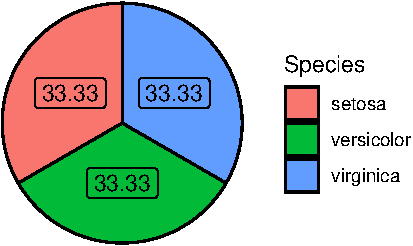
\includegraphics[keepaspectratio]{index_beamer_files/figure-beamer/unnamed-chunk-9-1.pdf}}
\end{frame}

\begin{frame}[fragile]{Gráfico de pontos}
\phantomsection\label{gruxe1fico-de-pontos}
\begin{Shaded}
\begin{Highlighting}[]
\FunctionTok{ggplot}\NormalTok{(iris,}\FunctionTok{aes}\NormalTok{(}\AttributeTok{x=}\NormalTok{Sepal.Length, }\AttributeTok{y=}\NormalTok{Sepal.Width))}\SpecialCharTok{+}
  \FunctionTok{geom\_point}\NormalTok{()}
\end{Highlighting}
\end{Shaded}

\pandocbounded{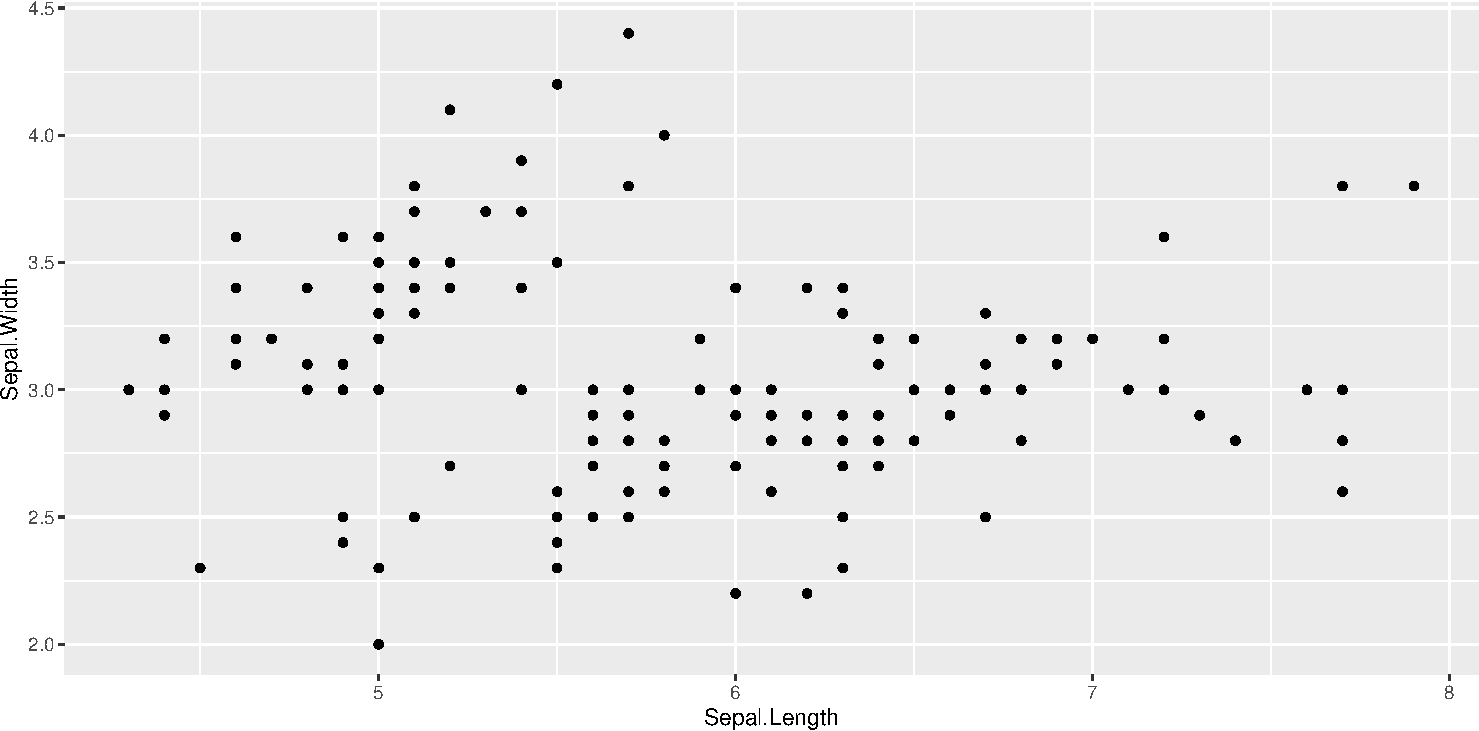
\includegraphics[keepaspectratio]{index_beamer_files/figure-beamer/unnamed-chunk-10-1.pdf}}
\end{frame}

\begin{frame}[fragile]
\begin{Shaded}
\begin{Highlighting}[]
\FunctionTok{ggplot}\NormalTok{(iris,}\FunctionTok{aes}\NormalTok{(}\AttributeTok{x=}\NormalTok{Sepal.Length, }\AttributeTok{y=}\NormalTok{Sepal.Width,}
                \AttributeTok{color=}\NormalTok{Species, }\AttributeTok{shape=}\NormalTok{Species))}\SpecialCharTok{+}
  \FunctionTok{geom\_point}\NormalTok{()}
\end{Highlighting}
\end{Shaded}

\pandocbounded{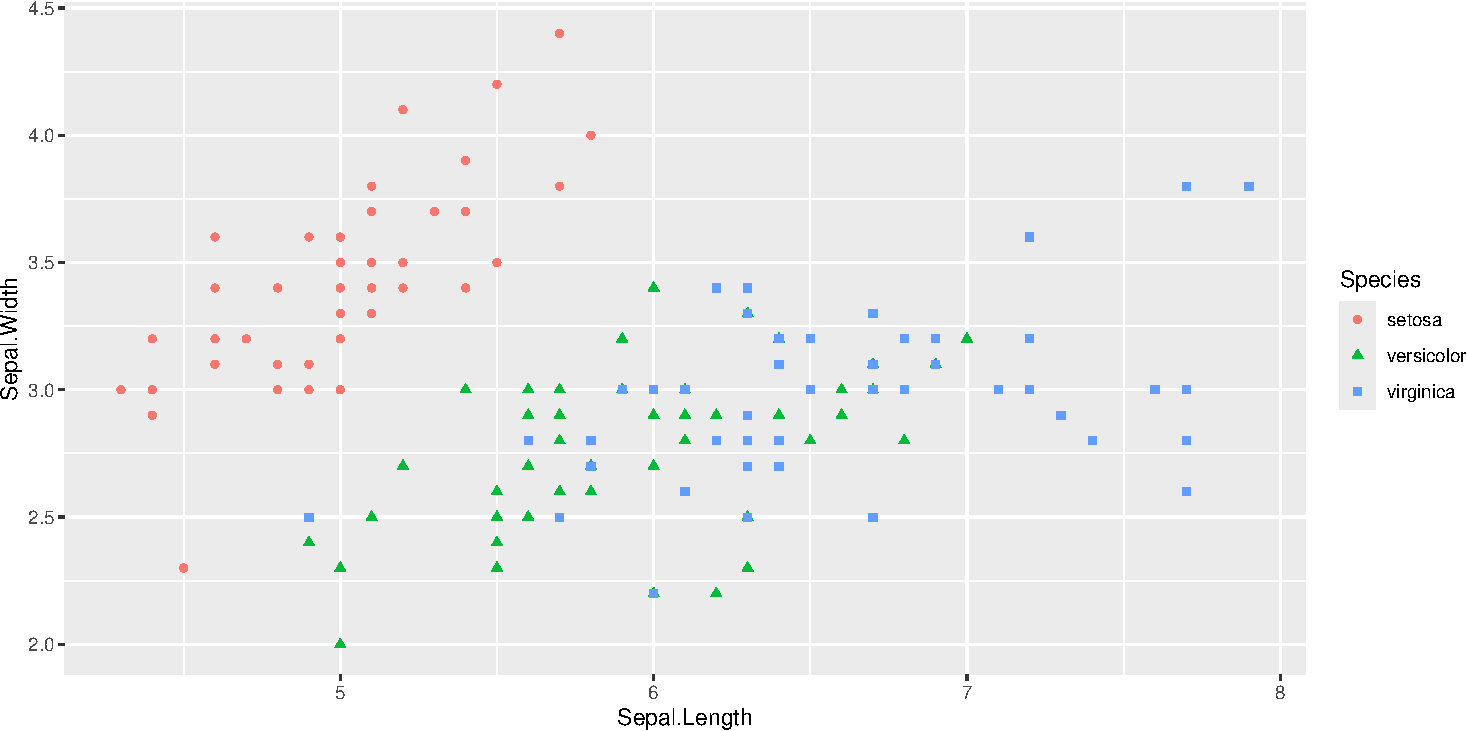
\includegraphics[keepaspectratio]{index_beamer_files/figure-beamer/unnamed-chunk-11-1.pdf}}
\end{frame}

\begin{frame}[fragile]
\begin{Shaded}
\begin{Highlighting}[]
\FunctionTok{ggplot}\NormalTok{(iris,}\FunctionTok{aes}\NormalTok{(}\AttributeTok{x=}\NormalTok{Sepal.Length, }\AttributeTok{y=}\NormalTok{Sepal.Width,}
                \AttributeTok{color=}\NormalTok{Species, }\AttributeTok{shape=}\NormalTok{Species))}\SpecialCharTok{+}
  \FunctionTok{geom\_point}\NormalTok{()}\SpecialCharTok{+}
  \FunctionTok{geom\_smooth}\NormalTok{(}\AttributeTok{se=}\ConstantTok{FALSE}\NormalTok{, }\AttributeTok{method=}\StringTok{"lm"}\NormalTok{)}
\end{Highlighting}
\end{Shaded}

\pandocbounded{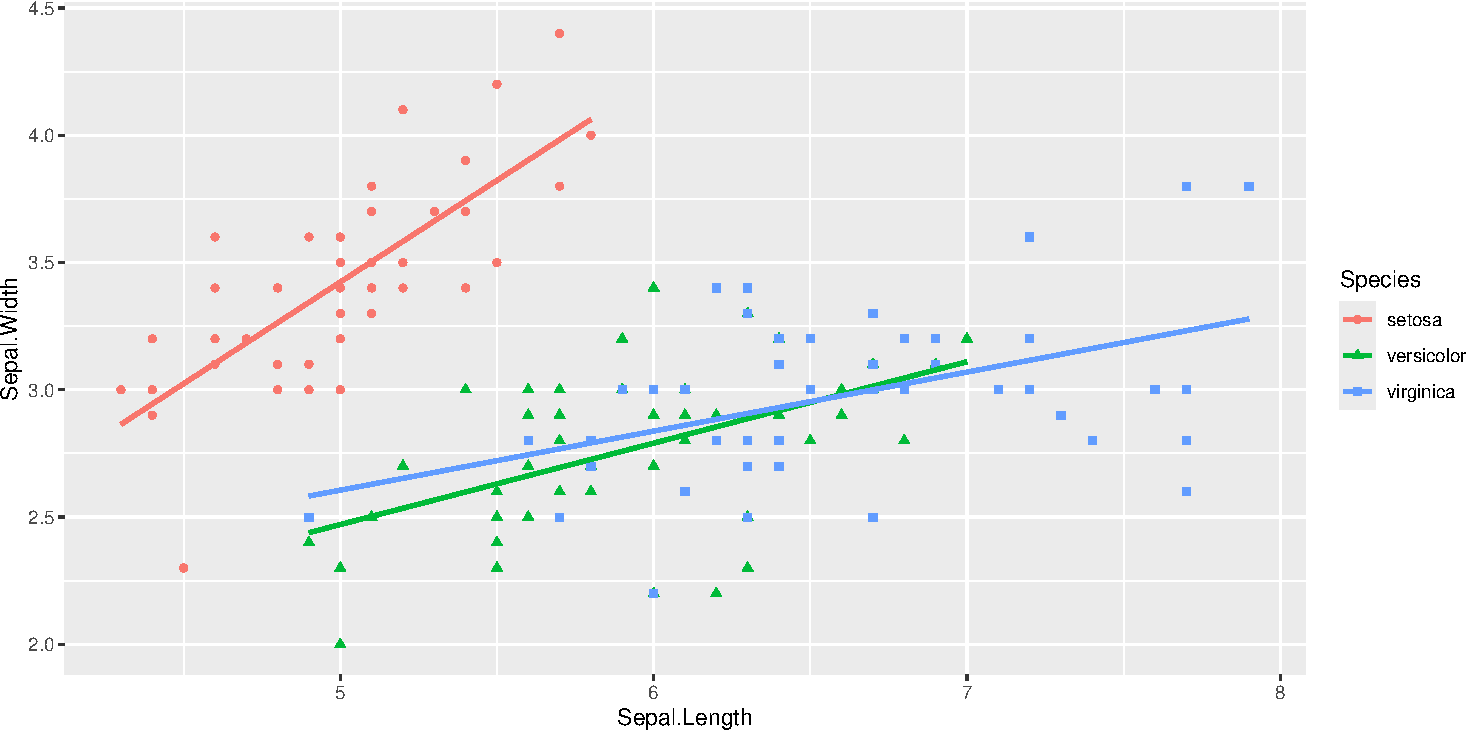
\includegraphics[keepaspectratio]{index_beamer_files/figure-beamer/unnamed-chunk-12-1.pdf}}
\end{frame}

\begin{frame}[fragile]
\begin{Shaded}
\begin{Highlighting}[]
\FunctionTok{ggplot}\NormalTok{(iris,}\FunctionTok{aes}\NormalTok{(}\AttributeTok{x=}\NormalTok{Sepal.Length, }\AttributeTok{y=}\NormalTok{Sepal.Width, }\AttributeTok{color=}\NormalTok{Species,}
                \AttributeTok{shape=}\NormalTok{Species))}\SpecialCharTok{+}
  \FunctionTok{geom\_point}\NormalTok{()}\SpecialCharTok{+}
  \FunctionTok{geom\_smooth}\NormalTok{(}\AttributeTok{se=}\ConstantTok{FALSE}\NormalTok{, }\AttributeTok{method=}\StringTok{"lm"}\NormalTok{)}\SpecialCharTok{+}
  \FunctionTok{coord\_flip}\NormalTok{()}
\end{Highlighting}
\end{Shaded}

\pandocbounded{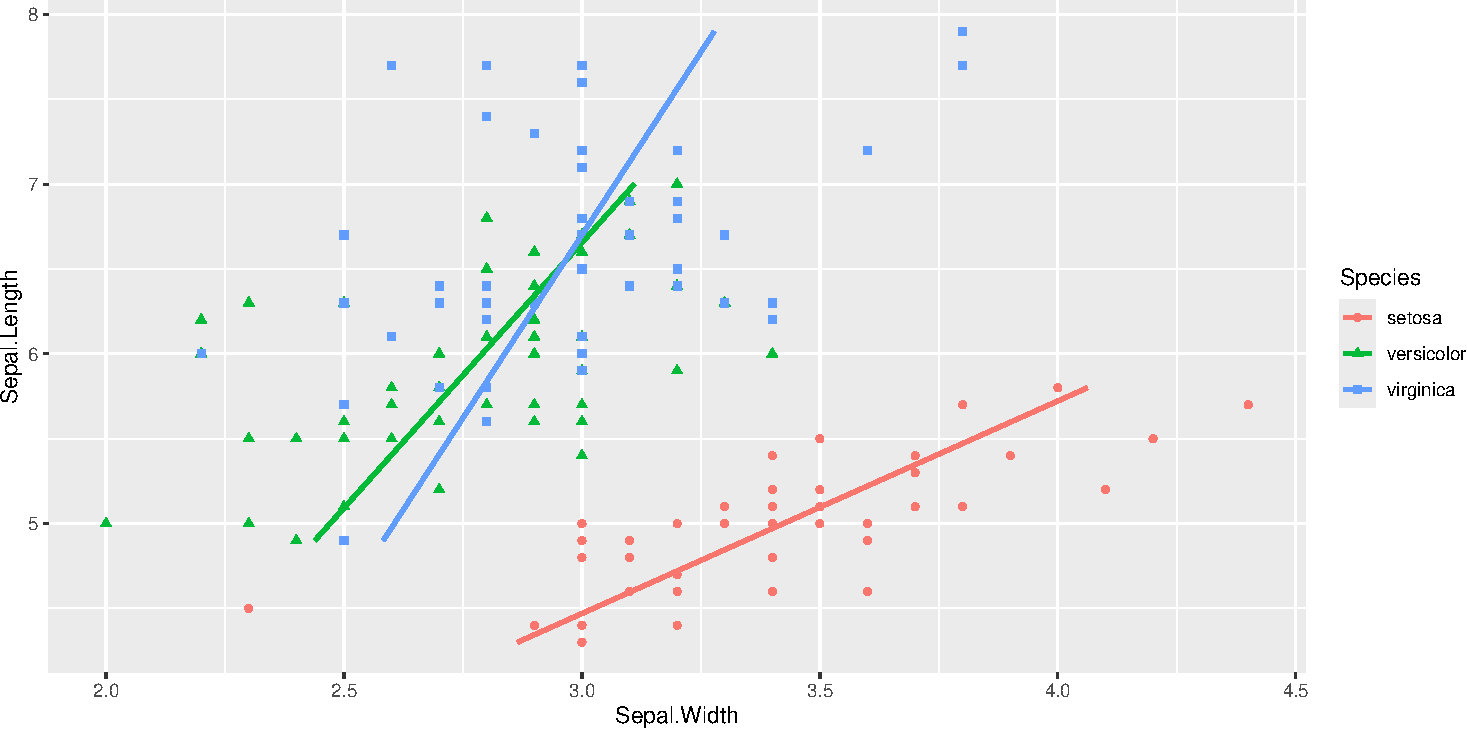
\includegraphics[keepaspectratio]{index_beamer_files/figure-beamer/unnamed-chunk-13-1.pdf}}
\end{frame}

\begin{frame}[fragile]{Gráfico de barras (média e desvio)}
\phantomsection\label{gruxe1fico-de-barras-muxe9dia-e-desvio}
\begin{Shaded}
\begin{Highlighting}[]
\NormalTok{iris}\SpecialCharTok{\%\textgreater{}\%}\FunctionTok{group\_by}\NormalTok{(Species)}\SpecialCharTok{\%\textgreater{}\%}
  \FunctionTok{summarise}\NormalTok{(}\AttributeTok{mean=}\FunctionTok{mean}\NormalTok{(Sepal.Length),}
            \AttributeTok{sd=}\FunctionTok{sd}\NormalTok{(Sepal.Length),}
            \AttributeTok{se=}\FunctionTok{sd}\NormalTok{(Sepal.Length)}\SpecialCharTok{/}\FunctionTok{sqrt}\NormalTok{(}\FunctionTok{length}\NormalTok{(Sepal.Length)))}\SpecialCharTok{\%\textgreater{}\%}
  \FunctionTok{ggplot}\NormalTok{(}\FunctionTok{aes}\NormalTok{(}\AttributeTok{x=}\NormalTok{Species, }\AttributeTok{y=}\NormalTok{mean))}\SpecialCharTok{+}
  \FunctionTok{geom\_col}\NormalTok{()}\SpecialCharTok{+}
  \FunctionTok{geom\_errorbar}\NormalTok{(}\FunctionTok{aes}\NormalTok{(}\AttributeTok{ymin=}\NormalTok{mean}\SpecialCharTok{{-}}\NormalTok{sd,}\AttributeTok{ymax=}\NormalTok{mean}\SpecialCharTok{+}\NormalTok{sd), }\AttributeTok{width=}\FloatTok{0.5}\NormalTok{)}\SpecialCharTok{+}
  \FunctionTok{labs}\NormalTok{(}\AttributeTok{y=}\StringTok{"Comprimento da Sepala"}\NormalTok{, }\AttributeTok{x=}\StringTok{"Espécies"}\NormalTok{)}\SpecialCharTok{+}
  \FunctionTok{theme\_bw}\NormalTok{()}\SpecialCharTok{+}
  \FunctionTok{scale\_y\_continuous}\NormalTok{(}\AttributeTok{limits=}\FunctionTok{c}\NormalTok{(}\DecValTok{0}\NormalTok{,}\DecValTok{10}\NormalTok{))}
\end{Highlighting}
\end{Shaded}

\pandocbounded{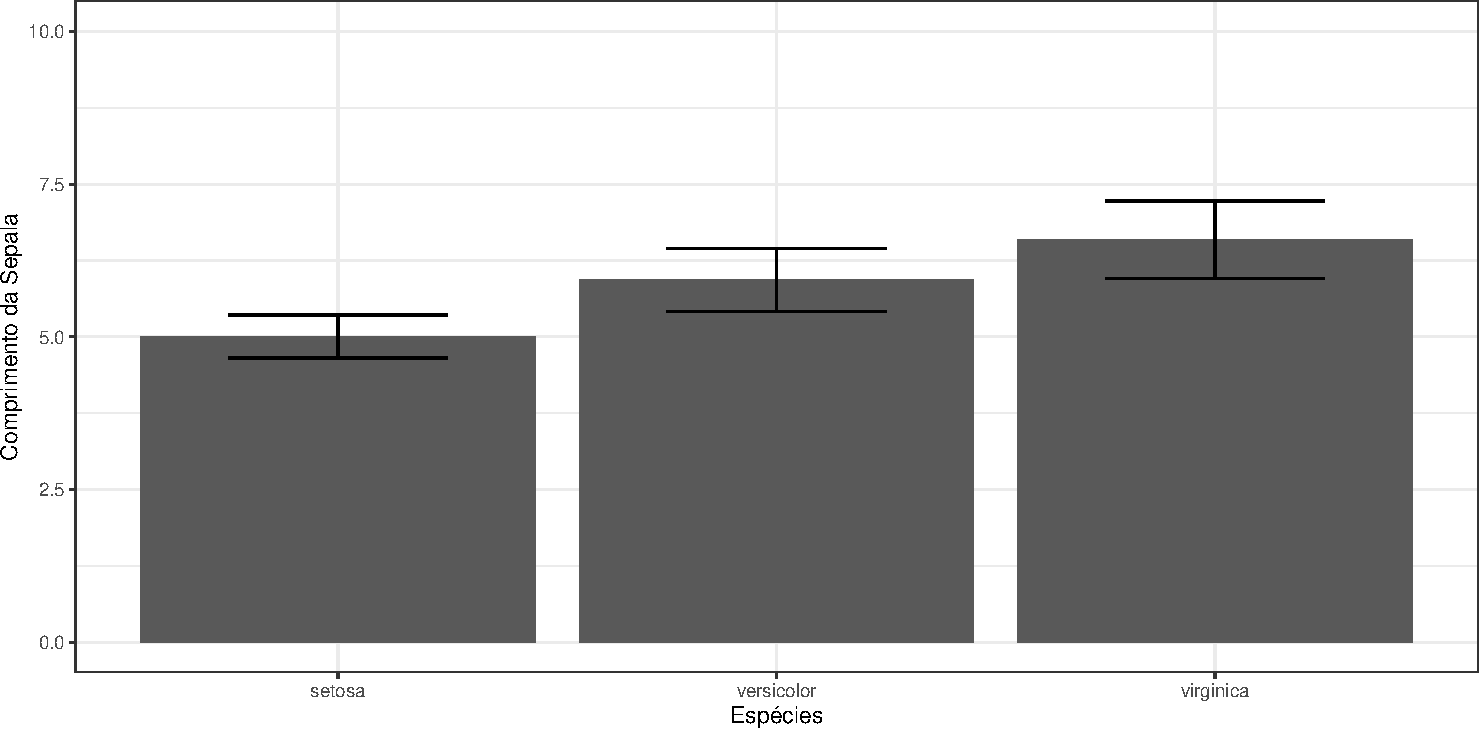
\includegraphics[keepaspectratio]{index_beamer_files/figure-beamer/grafico de barras-1.pdf}}
\end{frame}

\begin{frame}[fragile]
\begin{Shaded}
\begin{Highlighting}[]
\NormalTok{iris}\SpecialCharTok{\%\textgreater{}\%}\FunctionTok{group\_by}\NormalTok{(Species)}\SpecialCharTok{\%\textgreater{}\%}
  \FunctionTok{summarise}\NormalTok{(}\AttributeTok{mean=}\FunctionTok{mean}\NormalTok{(Sepal.Length),}
            \AttributeTok{sd=}\FunctionTok{sd}\NormalTok{(Sepal.Length),}
            \AttributeTok{se=}\FunctionTok{sd}\NormalTok{(Sepal.Length)}\SpecialCharTok{/}\FunctionTok{sqrt}\NormalTok{(}\FunctionTok{length}\NormalTok{(Sepal.Length)))}\SpecialCharTok{\%\textgreater{}\%}
  \FunctionTok{ggplot}\NormalTok{(}\FunctionTok{aes}\NormalTok{(}\AttributeTok{x=}\NormalTok{Species, }\AttributeTok{y=}\NormalTok{mean))}\SpecialCharTok{+}
  \FunctionTok{geom\_col}\NormalTok{()}\SpecialCharTok{+}
  \FunctionTok{geom\_linerange}\NormalTok{(}\FunctionTok{aes}\NormalTok{(}\AttributeTok{ymin=}\NormalTok{mean}\SpecialCharTok{{-}}\NormalTok{sd,}\AttributeTok{ymax=}\NormalTok{mean}\SpecialCharTok{+}\NormalTok{sd))}\SpecialCharTok{+}
  \FunctionTok{labs}\NormalTok{(}\AttributeTok{y=}\StringTok{"Comprimento da Sepala"}\NormalTok{, }\AttributeTok{x=}\StringTok{"Espécies"}\NormalTok{)}\SpecialCharTok{+}
  \FunctionTok{theme\_bw}\NormalTok{()}\SpecialCharTok{+}
  \FunctionTok{scale\_y\_continuous}\NormalTok{(}\AttributeTok{limits=}\FunctionTok{c}\NormalTok{(}\DecValTok{0}\NormalTok{,}\DecValTok{10}\NormalTok{))}
\end{Highlighting}
\end{Shaded}

\pandocbounded{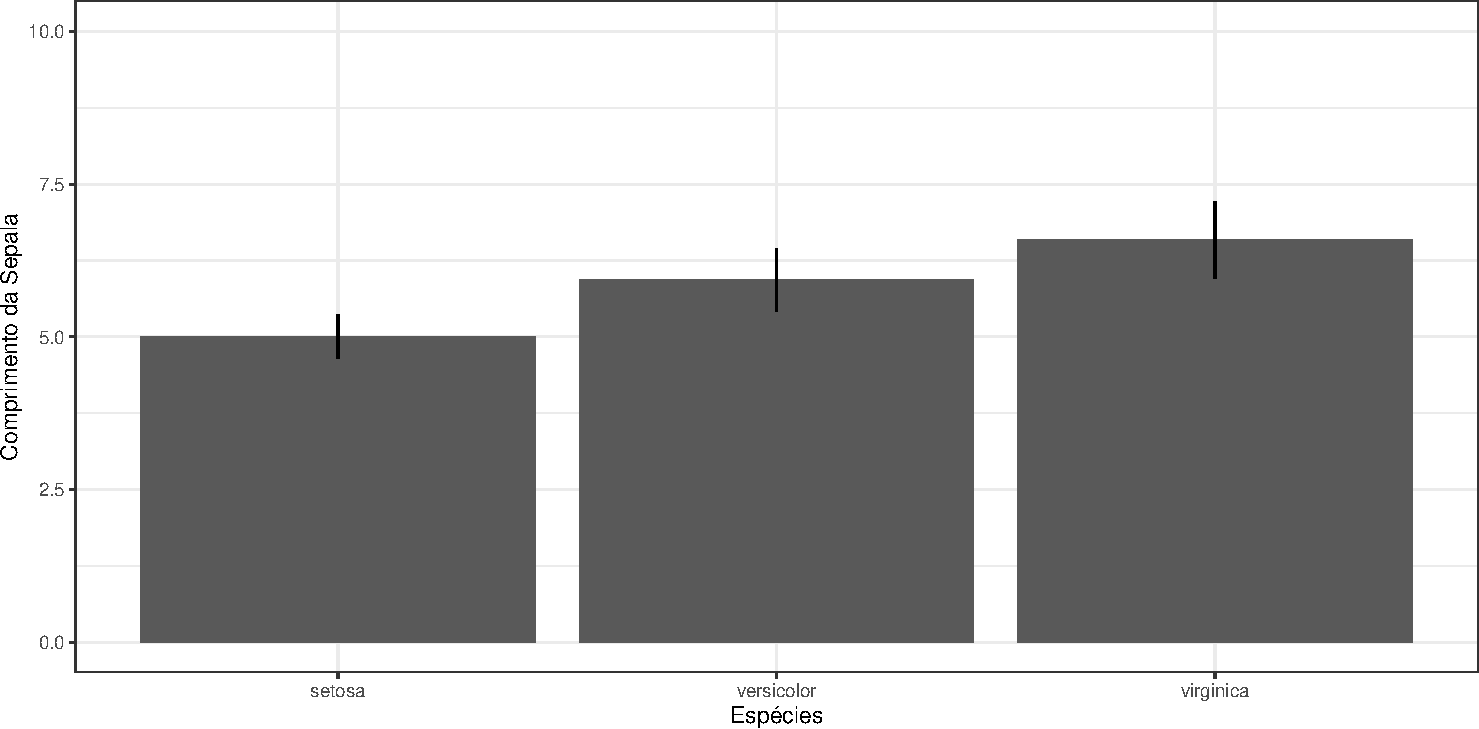
\includegraphics[keepaspectratio]{index_beamer_files/figure-beamer/unnamed-chunk-14-1.pdf}}
\end{frame}

\begin{frame}[fragile]
\begin{Shaded}
\begin{Highlighting}[]
\NormalTok{iris}\SpecialCharTok{\%\textgreater{}\%}\FunctionTok{group\_by}\NormalTok{(Species)}\SpecialCharTok{\%\textgreater{}\%}
  \FunctionTok{summarise}\NormalTok{(}\AttributeTok{mean=}\FunctionTok{mean}\NormalTok{(Sepal.Length), }\AttributeTok{sd=}\FunctionTok{sd}\NormalTok{(Sepal.Length),}\AttributeTok{se=}\FunctionTok{sd}\NormalTok{(Sepal.Length)}\SpecialCharTok{/}\FunctionTok{sqrt}\NormalTok{(}\FunctionTok{length}\NormalTok{(Sepal.Length)))}\SpecialCharTok{\%\textgreater{}\%}\FunctionTok{ggplot}\NormalTok{(}\FunctionTok{aes}\NormalTok{(}\AttributeTok{x=}\NormalTok{Species, }\AttributeTok{y=}\NormalTok{mean))}\SpecialCharTok{+}\FunctionTok{geom\_col}\NormalTok{()}\SpecialCharTok{+}\FunctionTok{geom\_pointrange}\NormalTok{(}\FunctionTok{aes}\NormalTok{(}\AttributeTok{ymin=}\NormalTok{mean}\SpecialCharTok{{-}}\NormalTok{sd,}\AttributeTok{ymax=}\NormalTok{mean}\SpecialCharTok{+}\NormalTok{sd))}\SpecialCharTok{+}\FunctionTok{labs}\NormalTok{(}\AttributeTok{y=}\StringTok{"Comprimento da Sepala"}\NormalTok{, }\AttributeTok{x=}\StringTok{"Espécies"}\NormalTok{)}\SpecialCharTok{+}\FunctionTok{theme\_bw}\NormalTok{()}\SpecialCharTok{+}\FunctionTok{scale\_y\_continuous}\NormalTok{(}\AttributeTok{limits=}\FunctionTok{c}\NormalTok{(}\DecValTok{0}\NormalTok{,}\DecValTok{10}\NormalTok{))}
\end{Highlighting}
\end{Shaded}

\pandocbounded{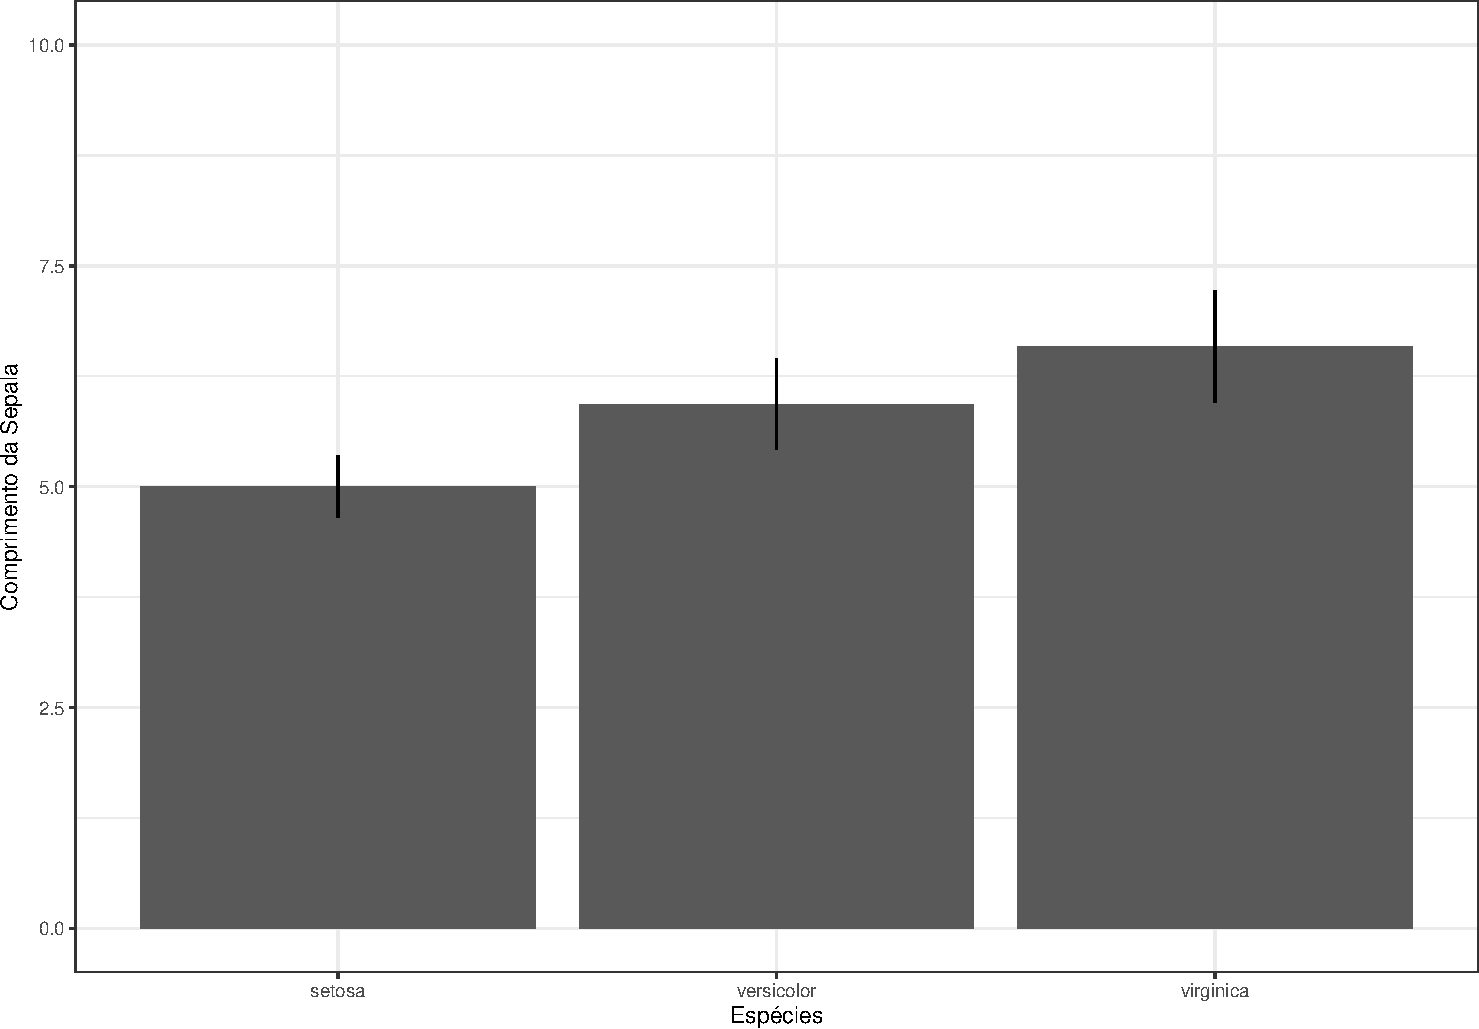
\includegraphics[keepaspectratio]{index_beamer_files/figure-beamer/unnamed-chunk-15-1.pdf}}
\end{frame}

\begin{frame}
\pandocbounded{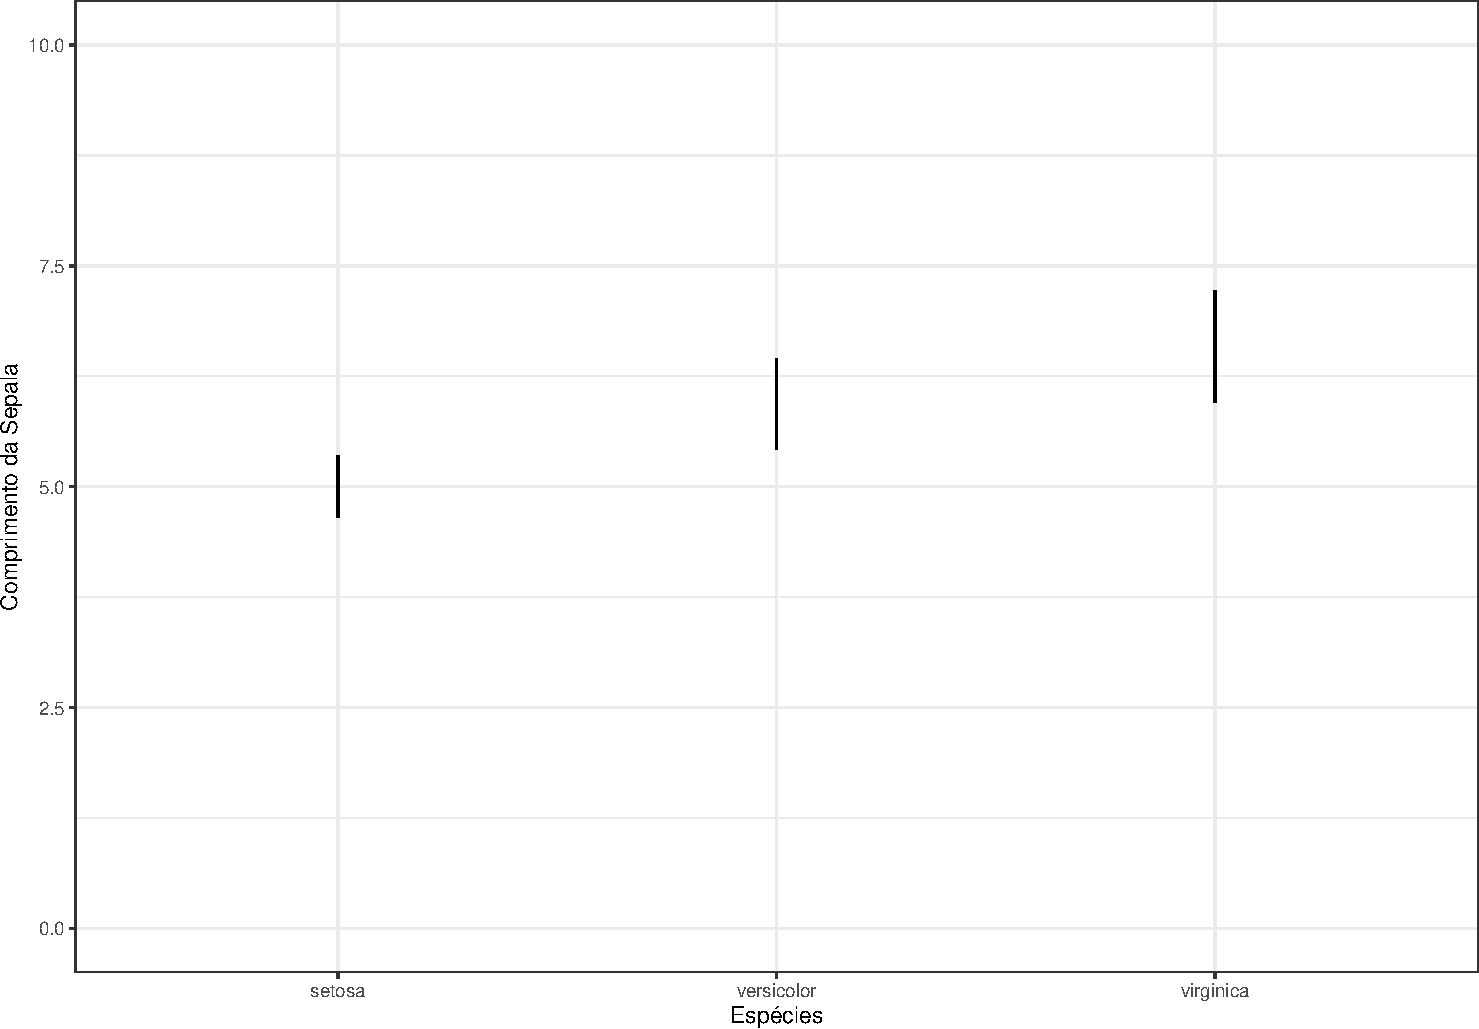
\includegraphics[keepaspectratio]{index_beamer_files/figure-beamer/unnamed-chunk-16-1.pdf}}
\end{frame}

\section{Alterando escalas, cores, fontes e
temas}\label{alterando-escalas-cores-fontes-e-temas}

\begin{frame}{Ajustando escalas no ggplot}
\phantomsection\label{ajustando-escalas-no-ggplot}
\pandocbounded{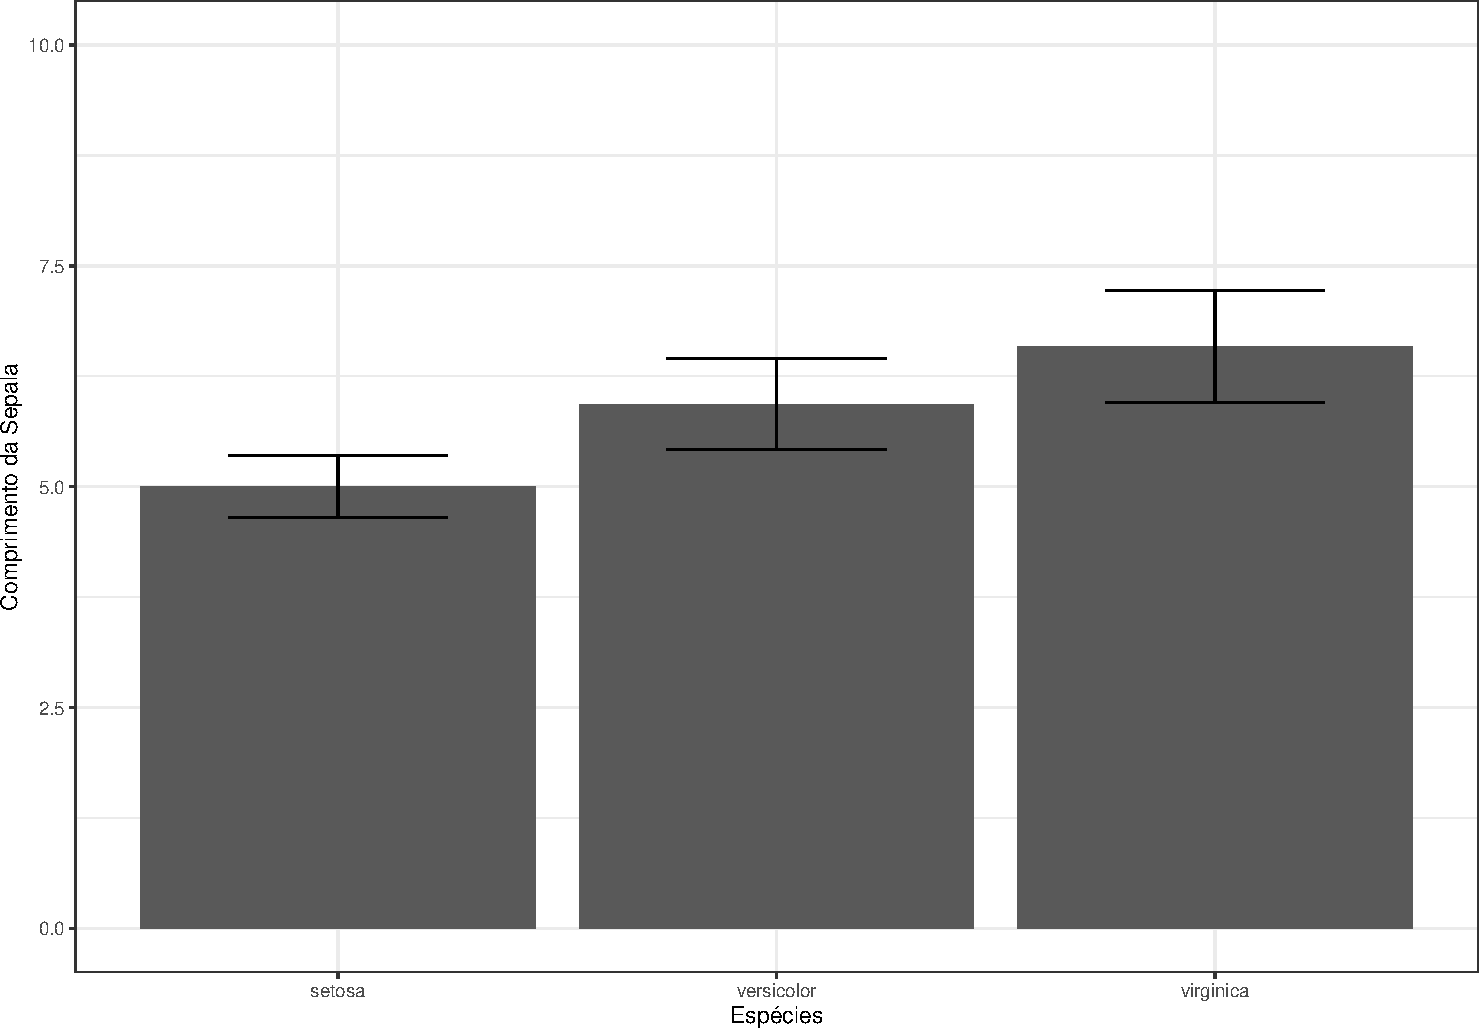
\includegraphics[keepaspectratio]{index_beamer_files/figure-beamer/escala-1.pdf}}
\end{frame}

\begin{frame}
\pandocbounded{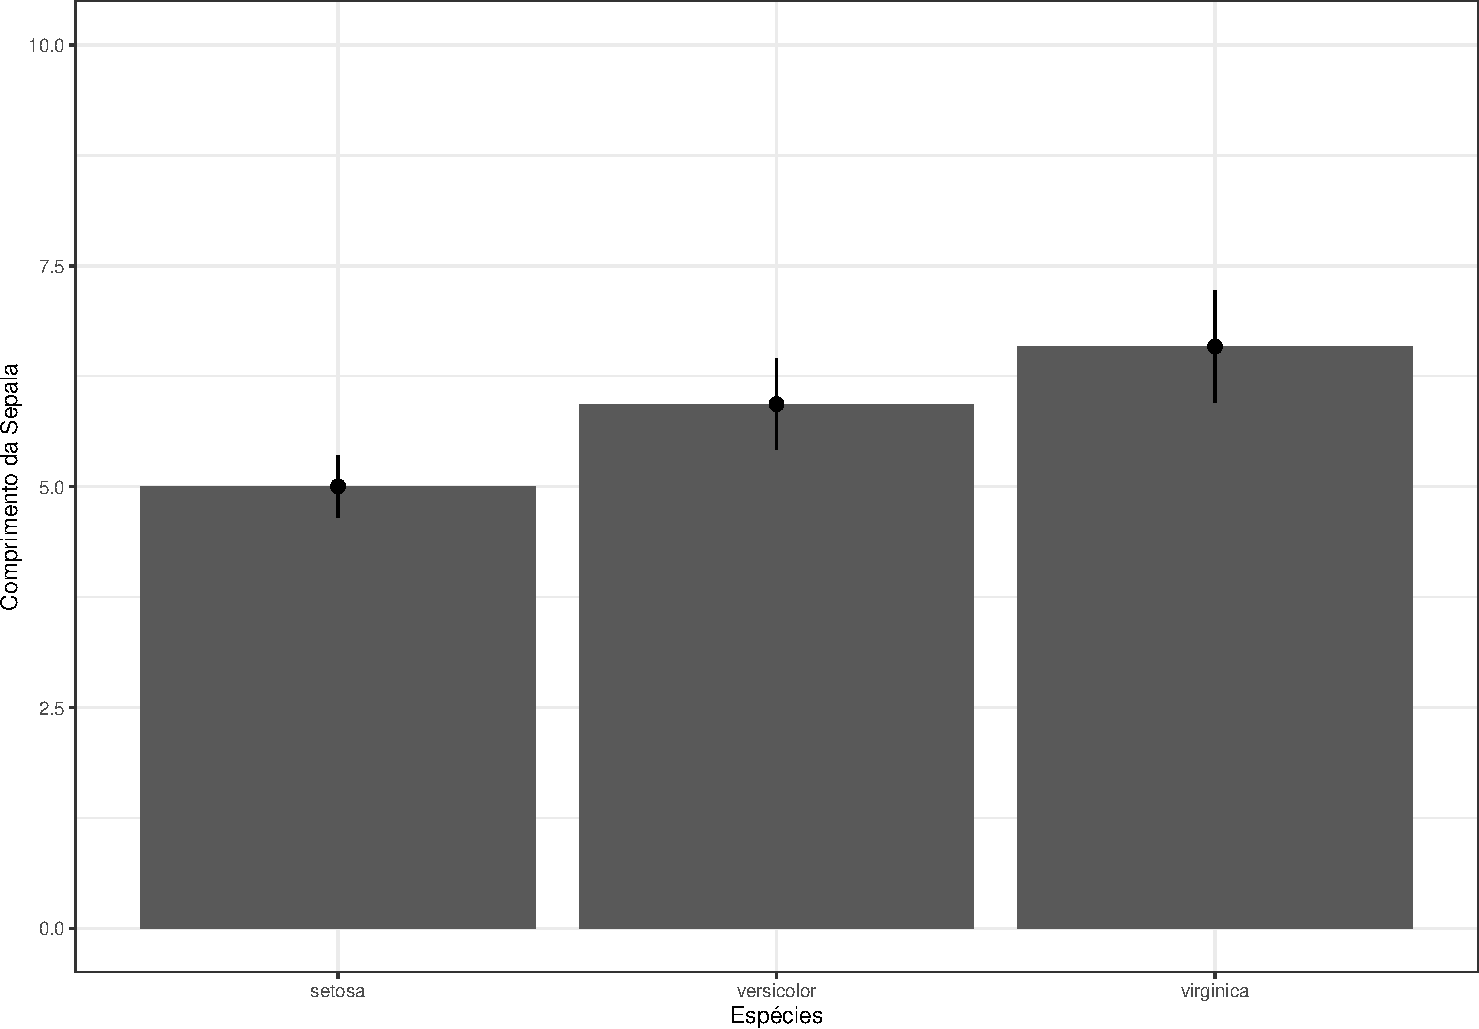
\includegraphics[keepaspectratio]{index_beamer_files/figure-beamer/unnamed-chunk-17-1.pdf}}
\end{frame}

\begin{frame}{Ordenando variáveis ordinais no ggplot}
\phantomsection\label{ordenando-variuxe1veis-ordinais-no-ggplot}
\pandocbounded{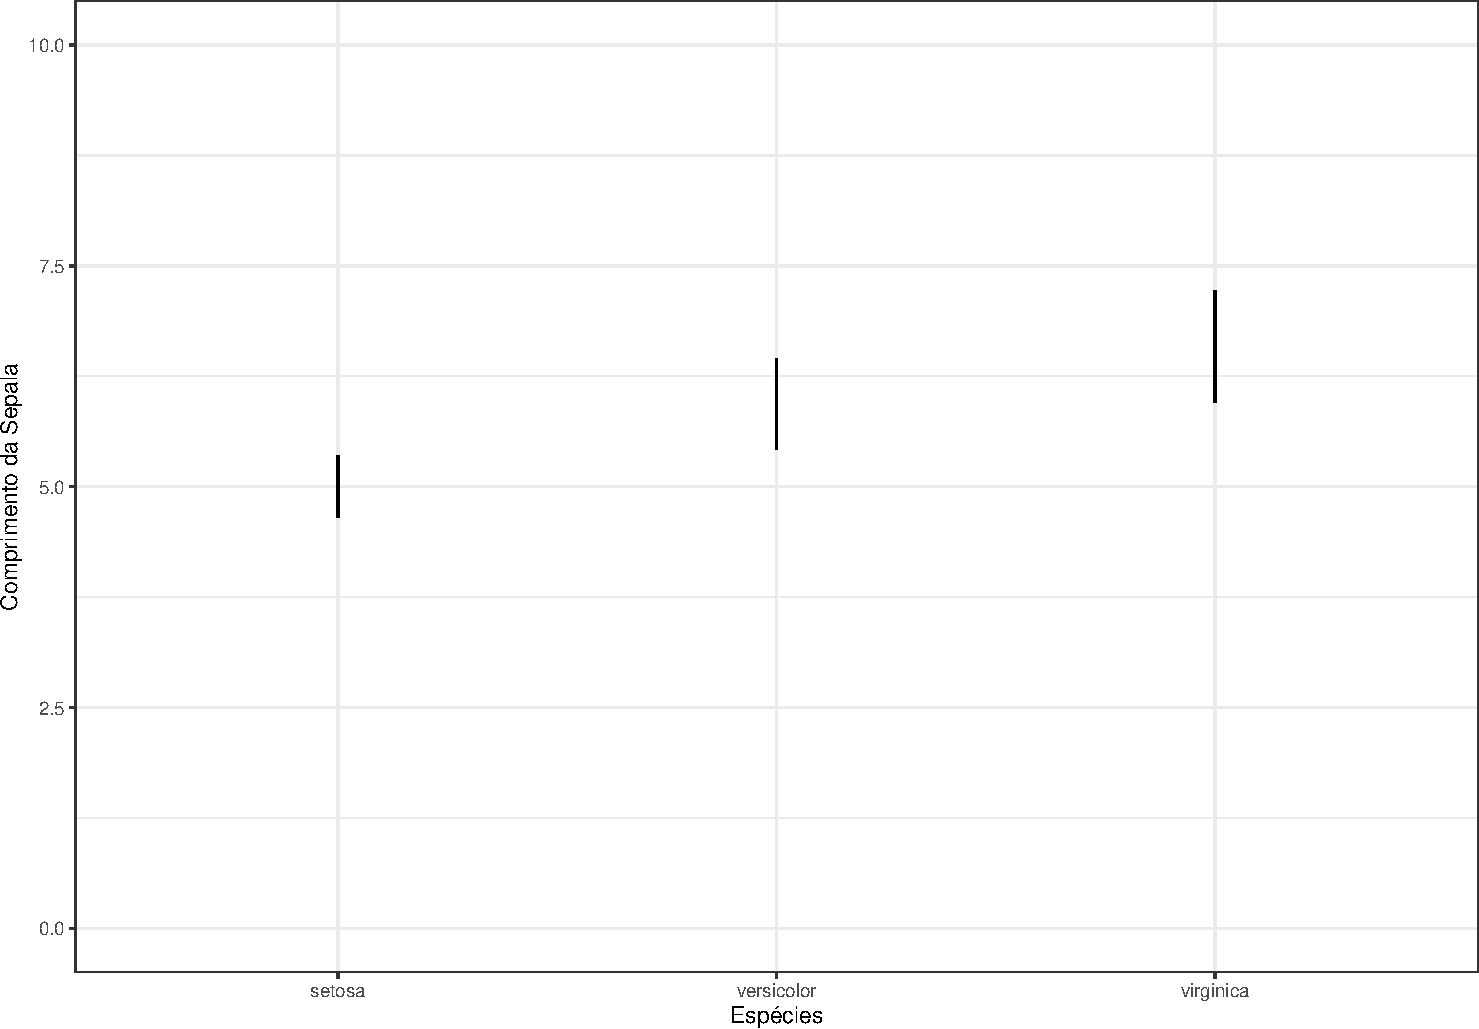
\includegraphics[keepaspectratio]{index_beamer_files/figure-beamer/unnamed-chunk-18-1.pdf}}
\end{frame}

\begin{frame}
\pandocbounded{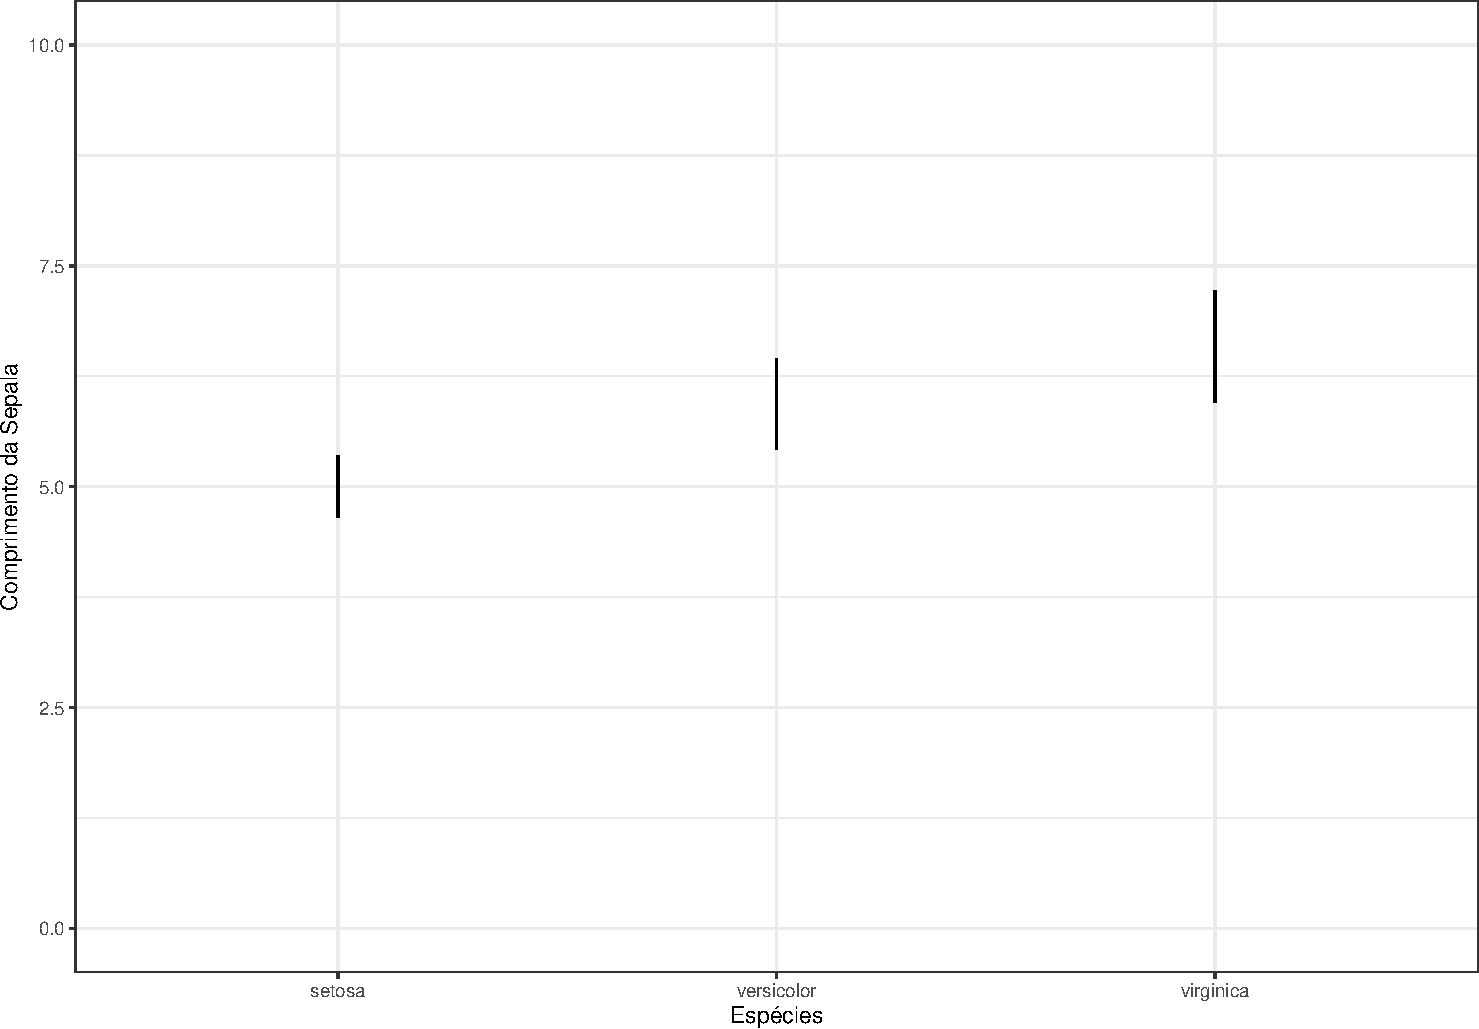
\includegraphics[keepaspectratio]{index_beamer_files/figure-beamer/unnamed-chunk-19-1.pdf}}
\end{frame}

\begin{frame}[fragile]{Mudando cores de preenchimento no ggplot}
\phantomsection\label{mudando-cores-de-preenchimento-no-ggplot}
\begin{Shaded}
\begin{Highlighting}[]
\NormalTok{iris}\SpecialCharTok{\%\textgreater{}\%}\FunctionTok{ggplot}\NormalTok{(}\FunctionTok{aes}\NormalTok{(}\AttributeTok{x=}\NormalTok{Species, }\AttributeTok{y=}\NormalTok{Petal.Length, }\AttributeTok{fill=}\NormalTok{Species))}\SpecialCharTok{+}
  \FunctionTok{geom\_boxplot}\NormalTok{()}
\end{Highlighting}
\end{Shaded}

\pandocbounded{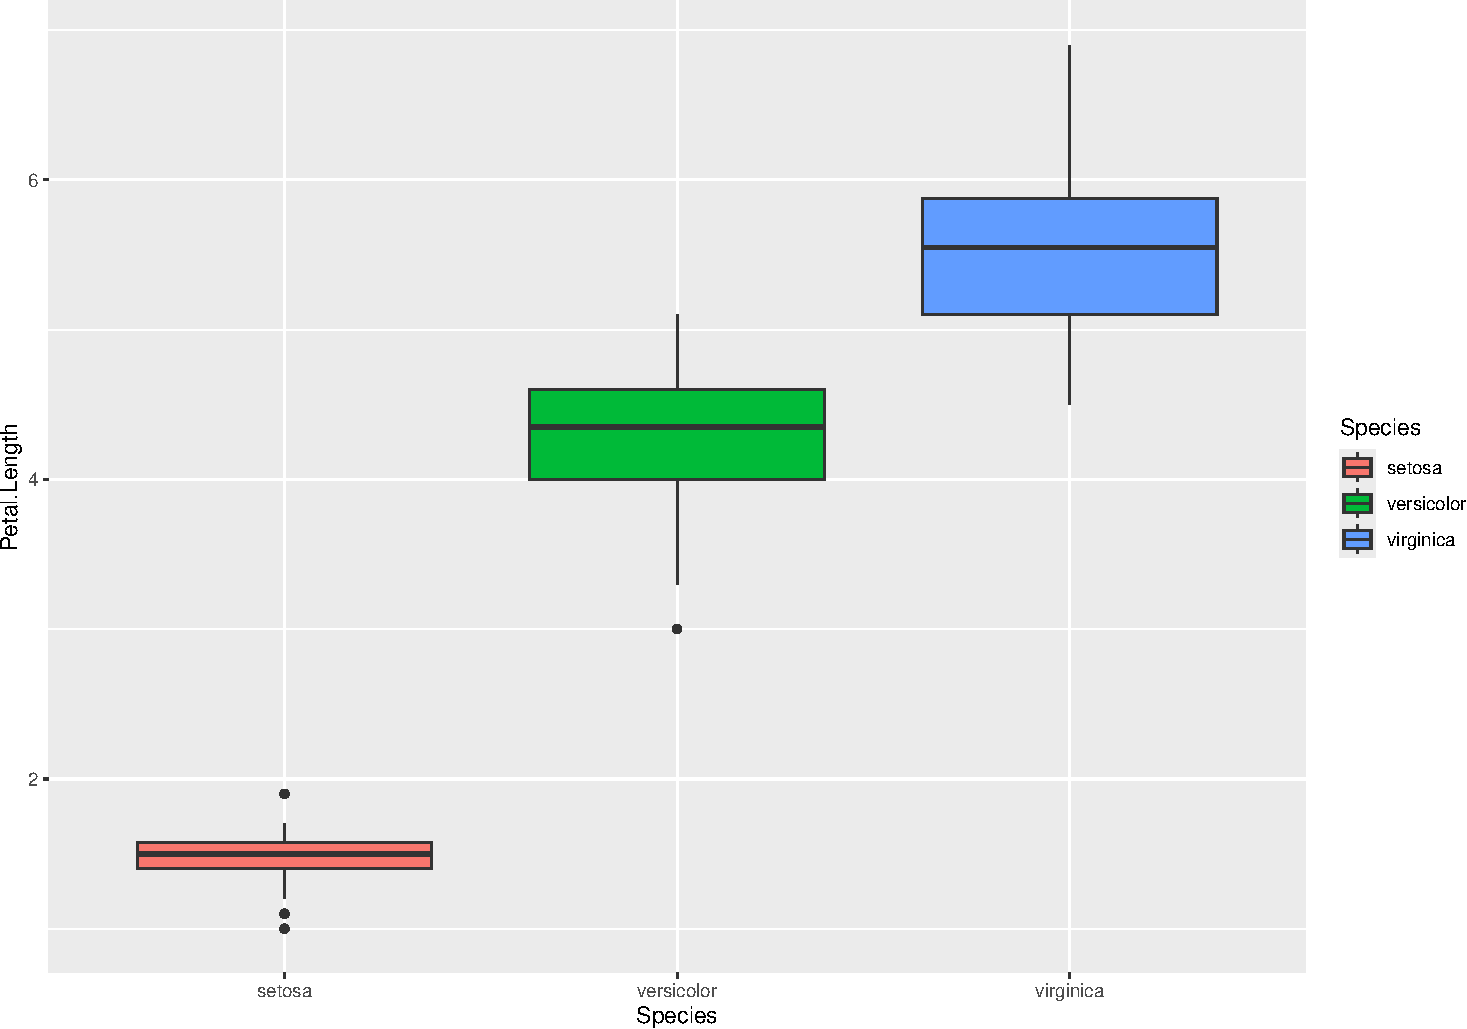
\includegraphics[keepaspectratio]{index_beamer_files/figure-beamer/Box-plot1-1.pdf}}
\end{frame}

\begin{frame}[fragile]
\begin{Shaded}
\begin{Highlighting}[]
\NormalTok{iris}\SpecialCharTok{\%\textgreater{}\%}\FunctionTok{ggplot}\NormalTok{(}\FunctionTok{aes}\NormalTok{(}\AttributeTok{x=}\NormalTok{Species, }\AttributeTok{y=}\NormalTok{Petal.Length))}\SpecialCharTok{+}
  \FunctionTok{geom\_boxplot}\NormalTok{(}\AttributeTok{fill=}\FunctionTok{c}\NormalTok{(}\StringTok{"lightpink"}\NormalTok{,}\StringTok{"lightgreen"}\NormalTok{,}\StringTok{"lightblue"}\NormalTok{))}
\end{Highlighting}
\end{Shaded}

\pandocbounded{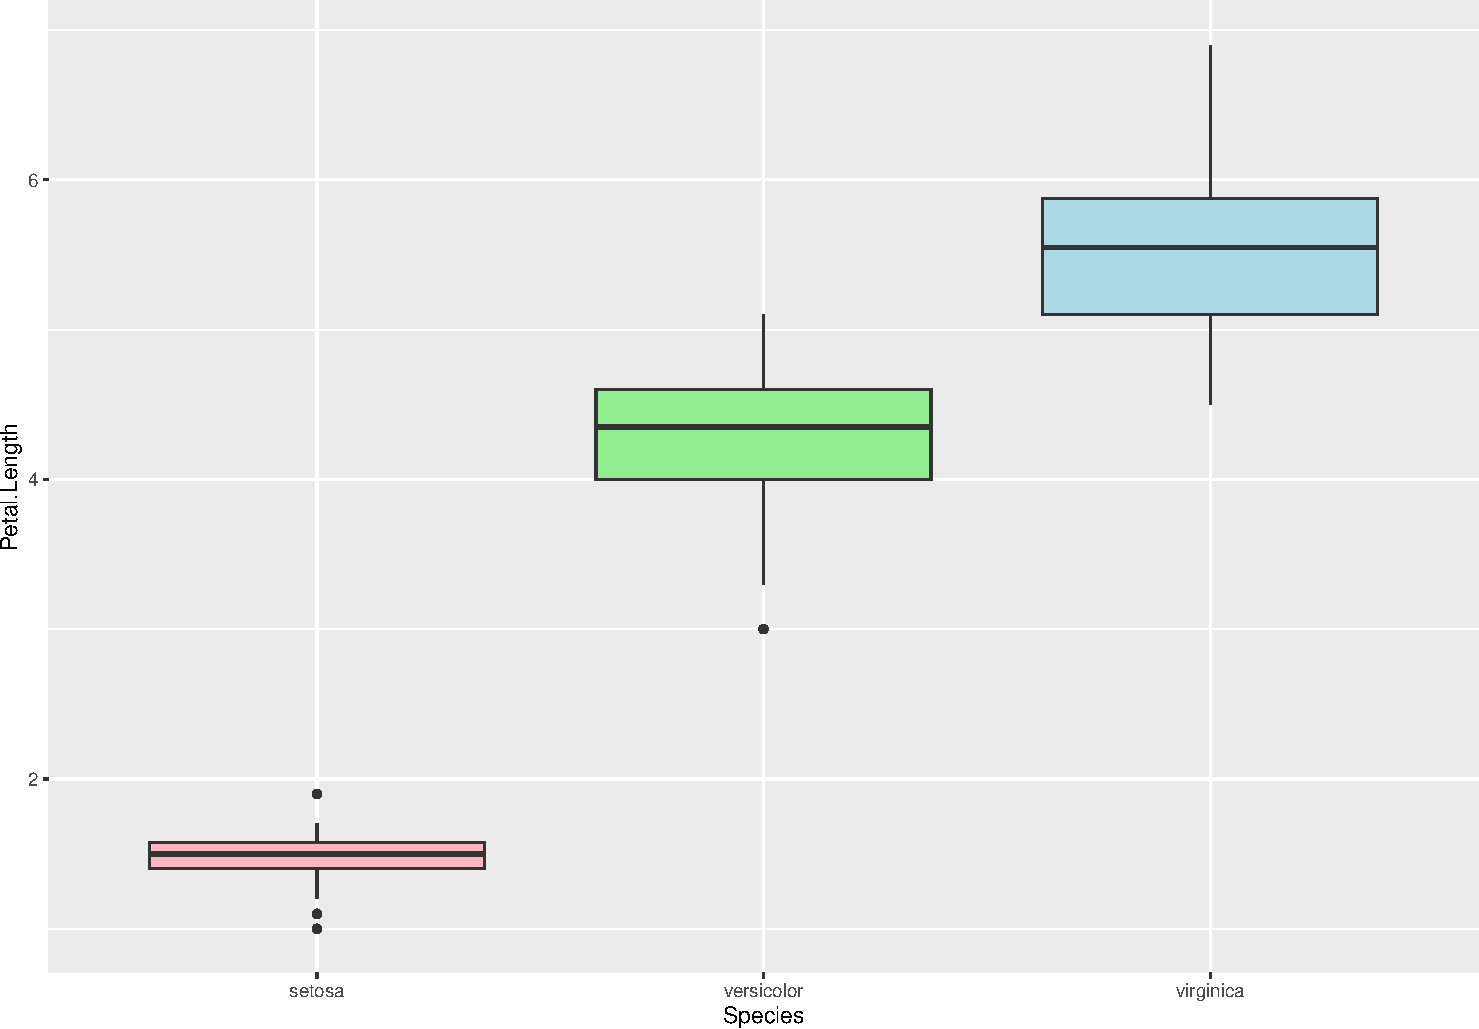
\includegraphics[keepaspectratio]{index_beamer_files/figure-beamer/Box-plot2-1.pdf}}
\end{frame}

\begin{frame}[fragile]
\begin{Shaded}
\begin{Highlighting}[]
\NormalTok{iris}\SpecialCharTok{\%\textgreater{}\%}\FunctionTok{ggplot}\NormalTok{(}\FunctionTok{aes}\NormalTok{(}\AttributeTok{x=}\NormalTok{Species, }\AttributeTok{y=}\NormalTok{Petal.Length, }\AttributeTok{fill=}\NormalTok{Species))}\SpecialCharTok{+}
  \FunctionTok{geom\_boxplot}\NormalTok{()}\SpecialCharTok{+}\FunctionTok{scale\_fill\_manual}\NormalTok{(}\AttributeTok{values=}\FunctionTok{c}\NormalTok{(}\StringTok{"\#704c41"}\NormalTok{,}\StringTok{"\#41704f"}\NormalTok{,}\StringTok{"\#584170"}\NormalTok{))}
\end{Highlighting}
\end{Shaded}

\pandocbounded{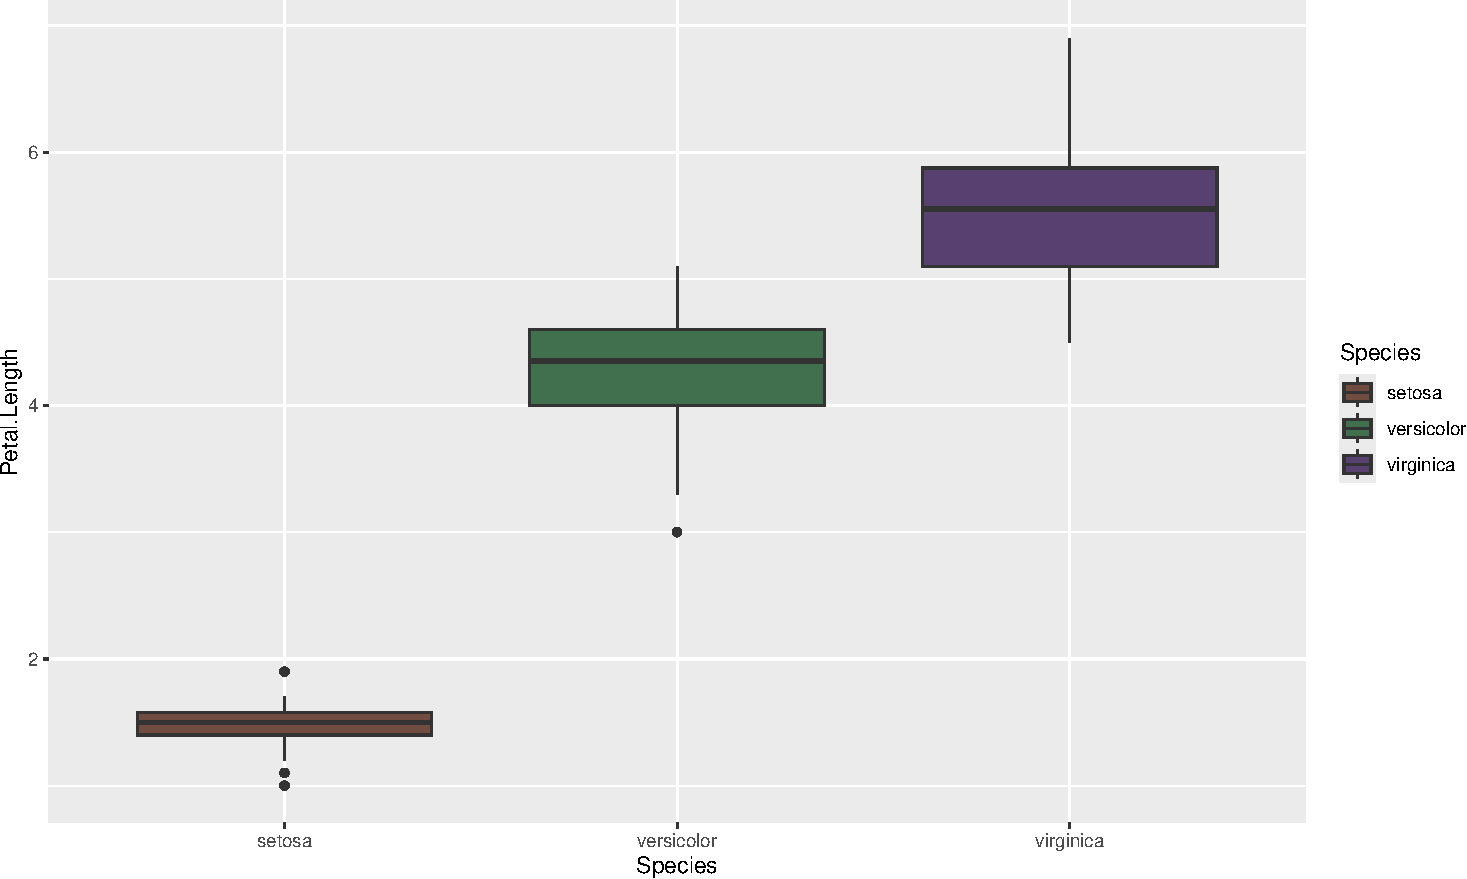
\includegraphics[keepaspectratio]{index_beamer_files/figure-beamer/Box-plot3-1.pdf}}
\end{frame}

\begin{frame}[fragile]{Mudando cores de contorno no ggplot}
\phantomsection\label{mudando-cores-de-contorno-no-ggplot}
\begin{Shaded}
\begin{Highlighting}[]
\NormalTok{iris}\SpecialCharTok{\%\textgreater{}\%}\FunctionTok{ggplot}\NormalTok{(}\FunctionTok{aes}\NormalTok{(}\AttributeTok{x=}\NormalTok{Species, }\AttributeTok{y=}\NormalTok{Petal.Length, }\AttributeTok{fill=}\NormalTok{Species))}\SpecialCharTok{+}\FunctionTok{geom\_boxplot}\NormalTok{(}\AttributeTok{fill=}\FunctionTok{c}\NormalTok{(}\StringTok{"lightblue"}\NormalTok{,}\StringTok{"lightgreen"}\NormalTok{,}\StringTok{"lightpink"}\NormalTok{), }\AttributeTok{color=}\StringTok{"brown"}\NormalTok{)}
\end{Highlighting}
\end{Shaded}

\pandocbounded{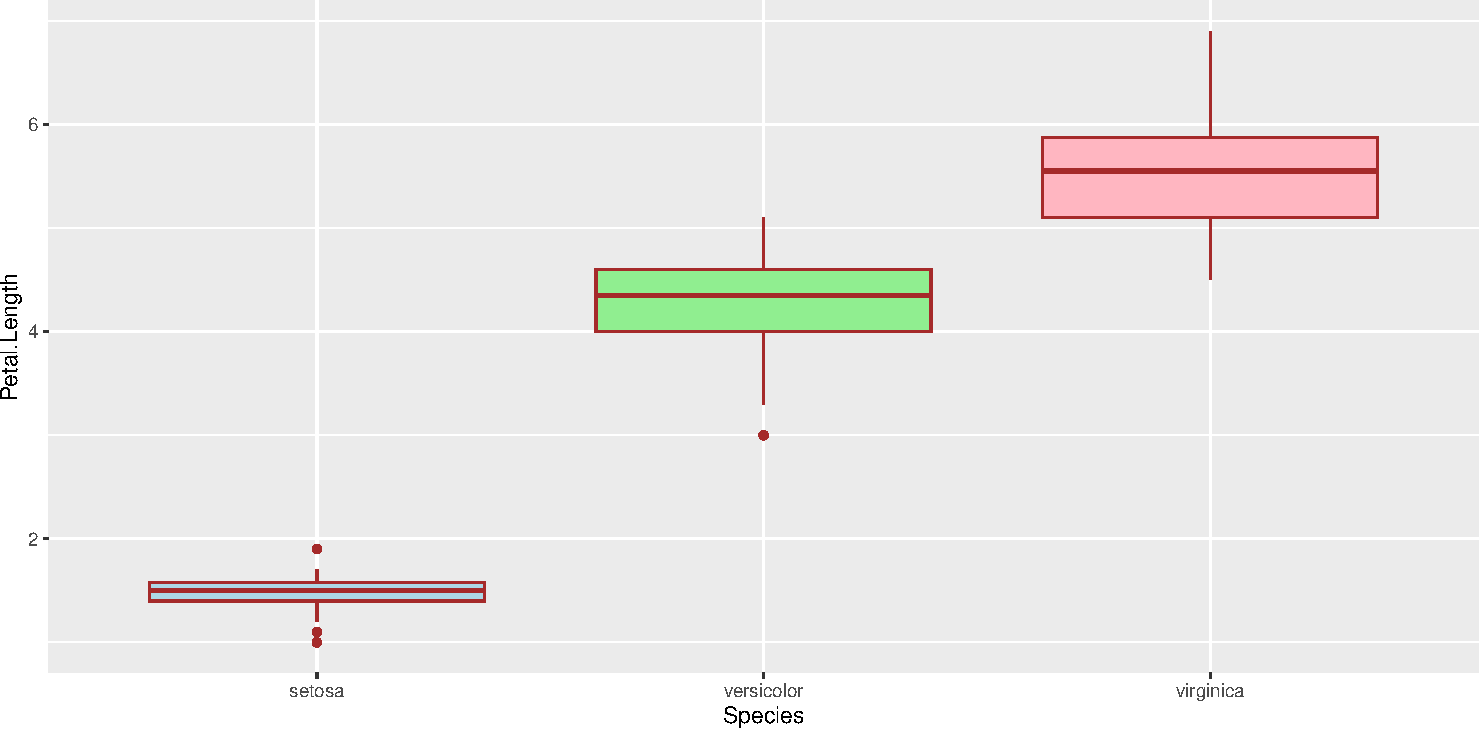
\includegraphics[keepaspectratio]{index_beamer_files/figure-beamer/Box-plot4-1.pdf}}
\end{frame}

\begin{frame}{Alterando elementos textuais no ggplot}
\phantomsection\label{alterando-elementos-textuais-no-ggplot}
Os nomes dos eixos são alterados pela função labs, onde você indica qual
elemento gráfico você quer renomear. Lembre-se: o nome que você quer
renomear tem que estar entre aspas \textbf{'' ``}.

\begin{itemize}
\tightlist
\item
  \textbf{y} para alterar o título do eixo y.
\item
  \textbf{x} para alterar o título do eixo x.
\item
  \textbf{title} para alterar o título ou acrescentar um título.
\item
  \textbf{subtitle} para alterar o subtítulo ou acrescentar um
  subtítulo.
\item
  \textbf{fill} para alterar o título da legenda referente ao fator
  colocado no fill.
\item
  \textbf{color} para alterar o título da legenda referente ao fator
  colocado no color.
\item
  \textbf{shape} para alterar o título da legenda referente ao fator
  colocado no shape.
\item
  \textbf{size} para alterar o título da legenda referente ao fator
  colocado no size.
\end{itemize}
\end{frame}

\begin{frame}[fragile]
\begin{Shaded}
\begin{Highlighting}[]
\NormalTok{iris}\SpecialCharTok{\%\textgreater{}\%}\FunctionTok{ggplot}\NormalTok{(}\FunctionTok{aes}\NormalTok{(}\AttributeTok{x=}\NormalTok{Species, }\AttributeTok{y=}\NormalTok{Petal.Length, }\AttributeTok{fill=}\NormalTok{Species))}\SpecialCharTok{+}
  \FunctionTok{geom\_boxplot}\NormalTok{(}\AttributeTok{fill=}\FunctionTok{c}\NormalTok{(}\StringTok{"lightblue"}\NormalTok{,}\StringTok{"lightgreen"}\NormalTok{,}\StringTok{"lightpink"}\NormalTok{), }\AttributeTok{color=}\StringTok{"brown"}\NormalTok{)}\SpecialCharTok{+}
  \FunctionTok{labs}\NormalTok{(}\AttributeTok{y=}\StringTok{"Comprimento de pétala"}\NormalTok{,}
       \AttributeTok{x=}\StringTok{"Espécies"}\NormalTok{,}
       \AttributeTok{title=}\StringTok{"Comparação de comprimento de pétalas"}\NormalTok{,}
       \AttributeTok{subtitle =} \StringTok{"Banco de dados iris"}\NormalTok{)}
\end{Highlighting}
\end{Shaded}

\pandocbounded{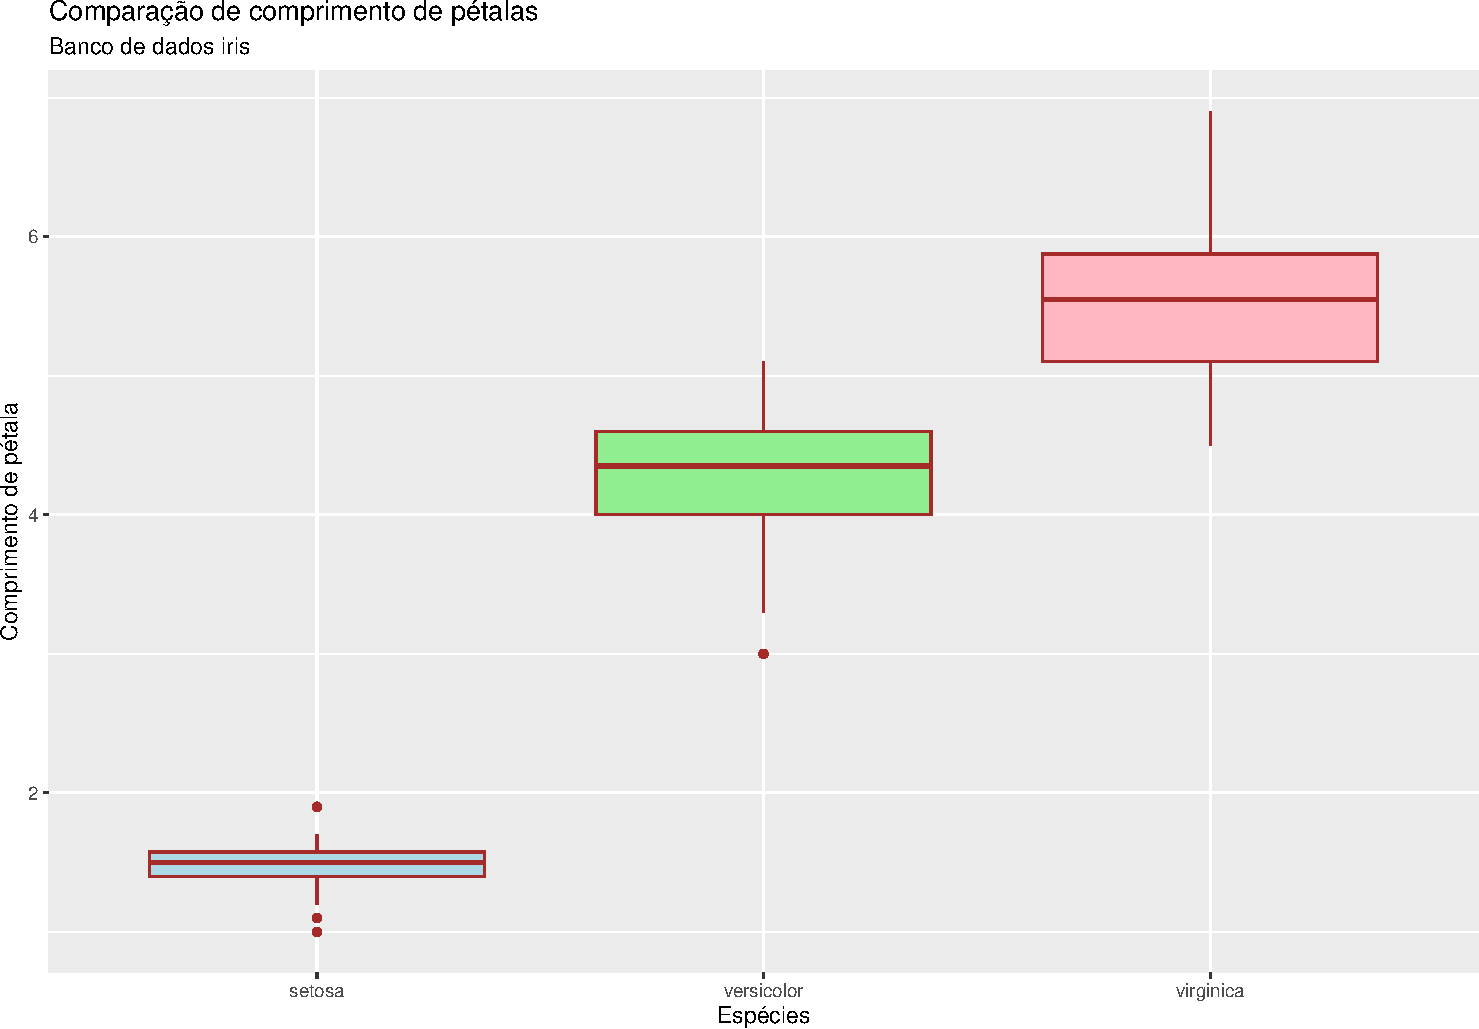
\includegraphics[keepaspectratio]{index_beamer_files/figure-beamer/Box-plot eixos-1.pdf}}

\begin{block}{Alterando a fonte}
\phantomsection\label{alterando-a-fonte}
Aqui alteramos as fontes através do comando \texttt{theme()} este
comando altera elementos temáticos do gráfico, como por exemplo fontes,
tamanhos, cor de fundo, entre outros. Neste exemplo colocamons o
argumento \texttt{text\ =\ element\_text()}. Dentro dele vai alguns
argumentos:

\begin{itemize}
\tightlist
\item
  \textbf{face} é para definir se a fonte estará em itálico
  (\texttt{"italic"}), negrito (\texttt{"bold"}) ou ambos
  (\texttt{"italic.bold"})
\item
  \textbf{family} é para definir se o tipo de fonte. Esse argumento pode
  ter variações de acordo com sistema operacional do computador. Em
  sistema windows pode-se utilizar \texttt{"TT\ Times\ New\ Roman"},
  \texttt{"Arial"}, etc. Enquanto em sistemas Linux e MacOS estarão
  \texttt{"serif"}, \texttt{"mono"}, etc.
\item
  \textbf{size} é para definir se o tamanho da fonte.
\end{itemize}

\pandocbounded{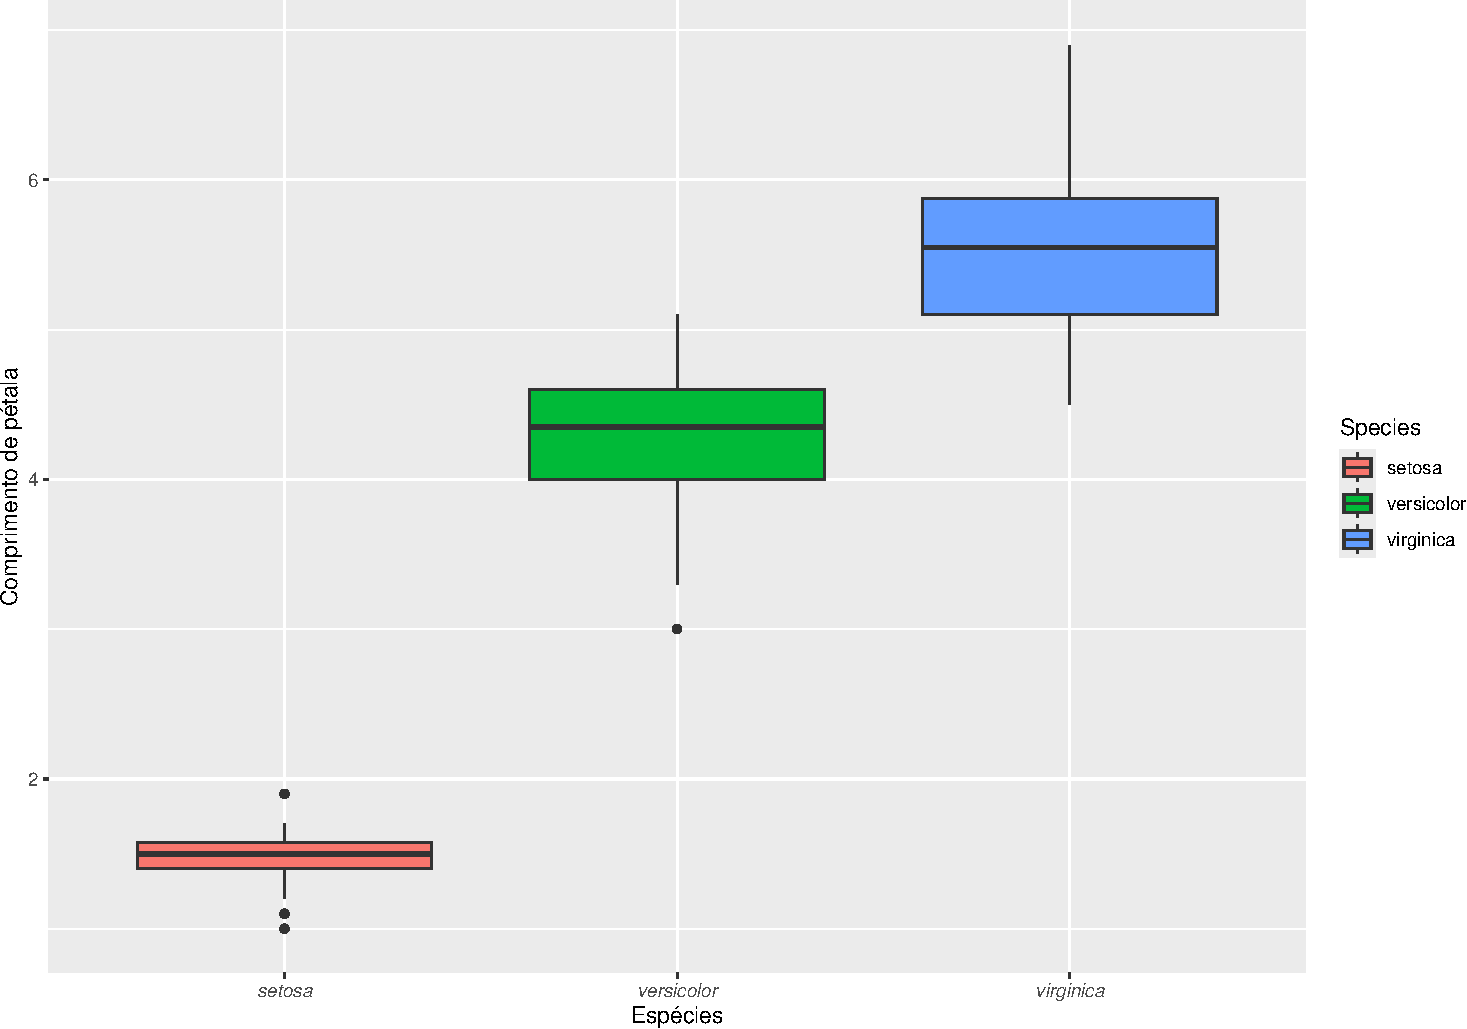
\includegraphics[keepaspectratio]{index_beamer_files/figure-beamer/unnamed-chunk-21-1.pdf}}

\pandocbounded{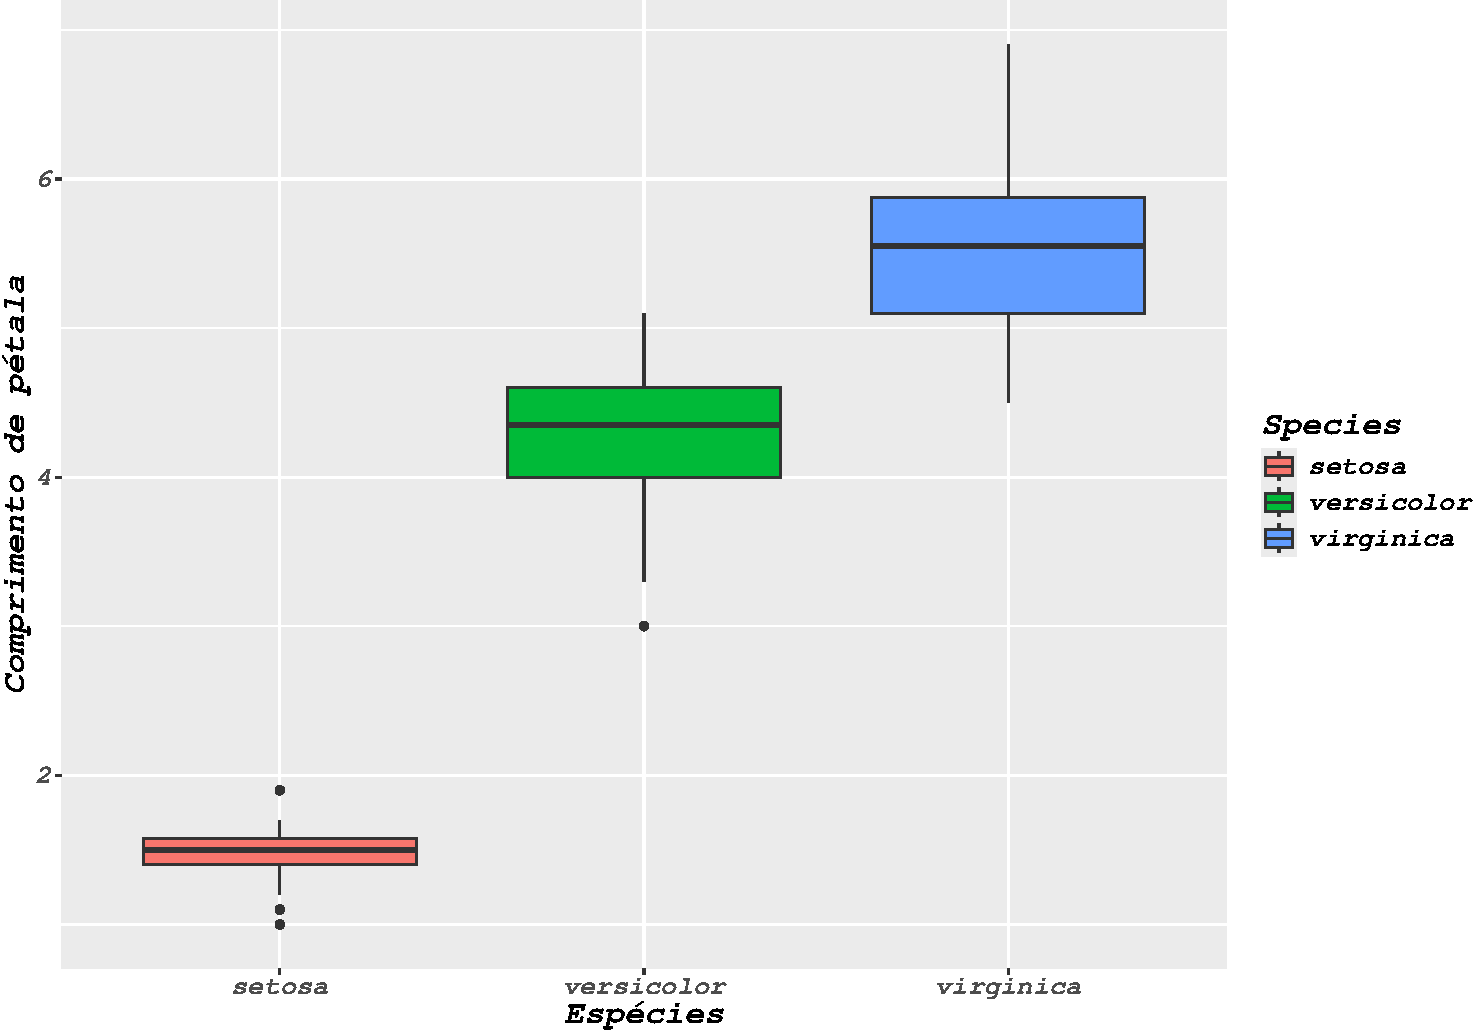
\includegraphics[keepaspectratio]{index_beamer_files/figure-beamer/unnamed-chunk-21-2.pdf}}

\pandocbounded{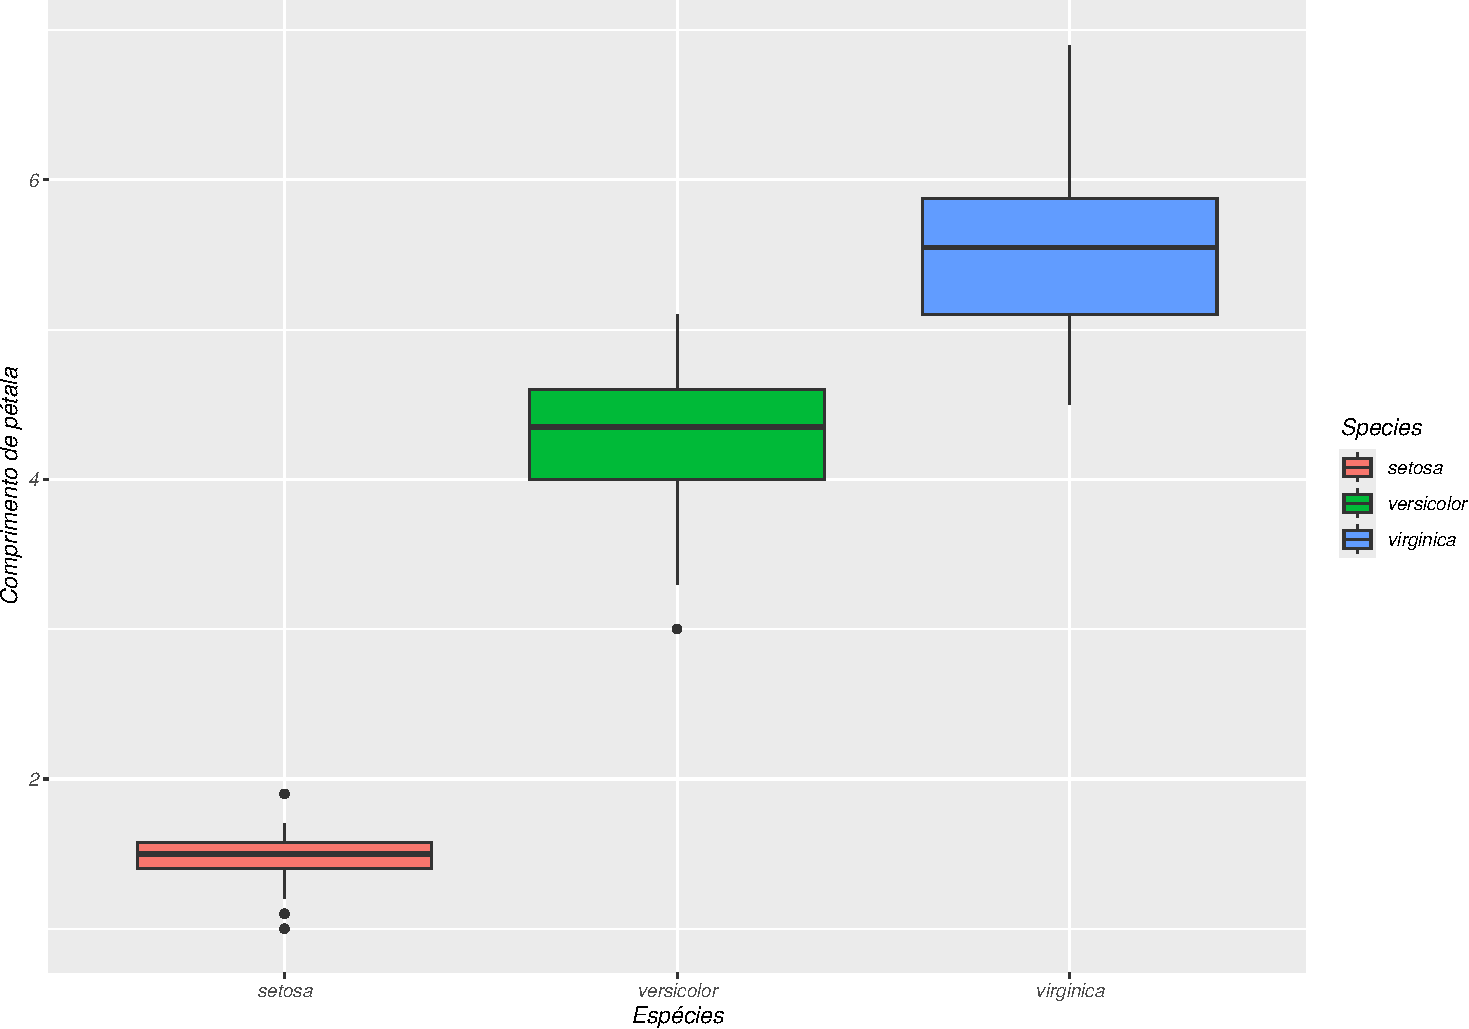
\includegraphics[keepaspectratio]{index_beamer_files/figure-beamer/unnamed-chunk-21-3.pdf}}

As vezes é necessário colocar nomes em itálico, como por exemplo nomes
de espécies que estão no eixo x. Com isso dentro de \texttt{theme()}
colocaremos o arguemento
\texttt{axis.text.x\ =\ element\_text(face="italic")} se referindo que
estaremos trabalhando com o texto presente na escala do eixo x. Caso
fosse no eixo y seria \texttt{axis.text.y}. Essa alteração também pode
ser aplicada à outros parâmetros, como \texttt{fill} e \texttt{color}.
Trabalhando assim, podemos alterar a fonte apenas daquele parâmetro.

\pandocbounded{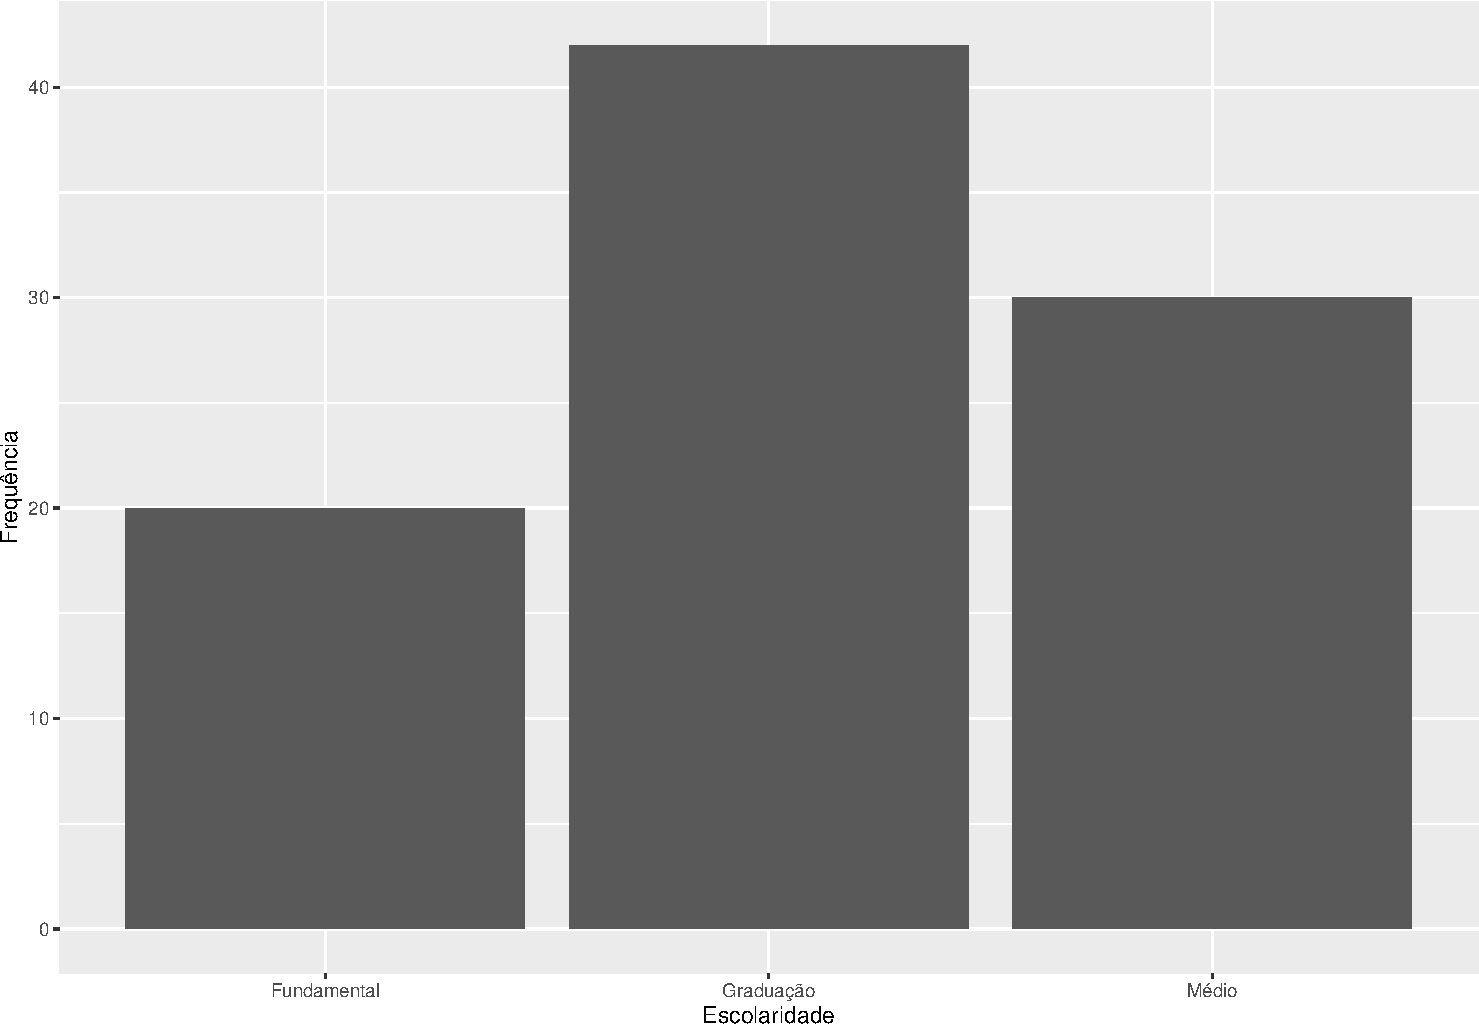
\includegraphics[keepaspectratio]{index_beamer_files/figure-beamer/unnamed-chunk-22-1.pdf}}

A seguir há o exemplo de deixar o título em negrito com maior destaque,
utilizando o argumento
\texttt{plot.title\ =\ element\_text(face="bold")}

\pandocbounded{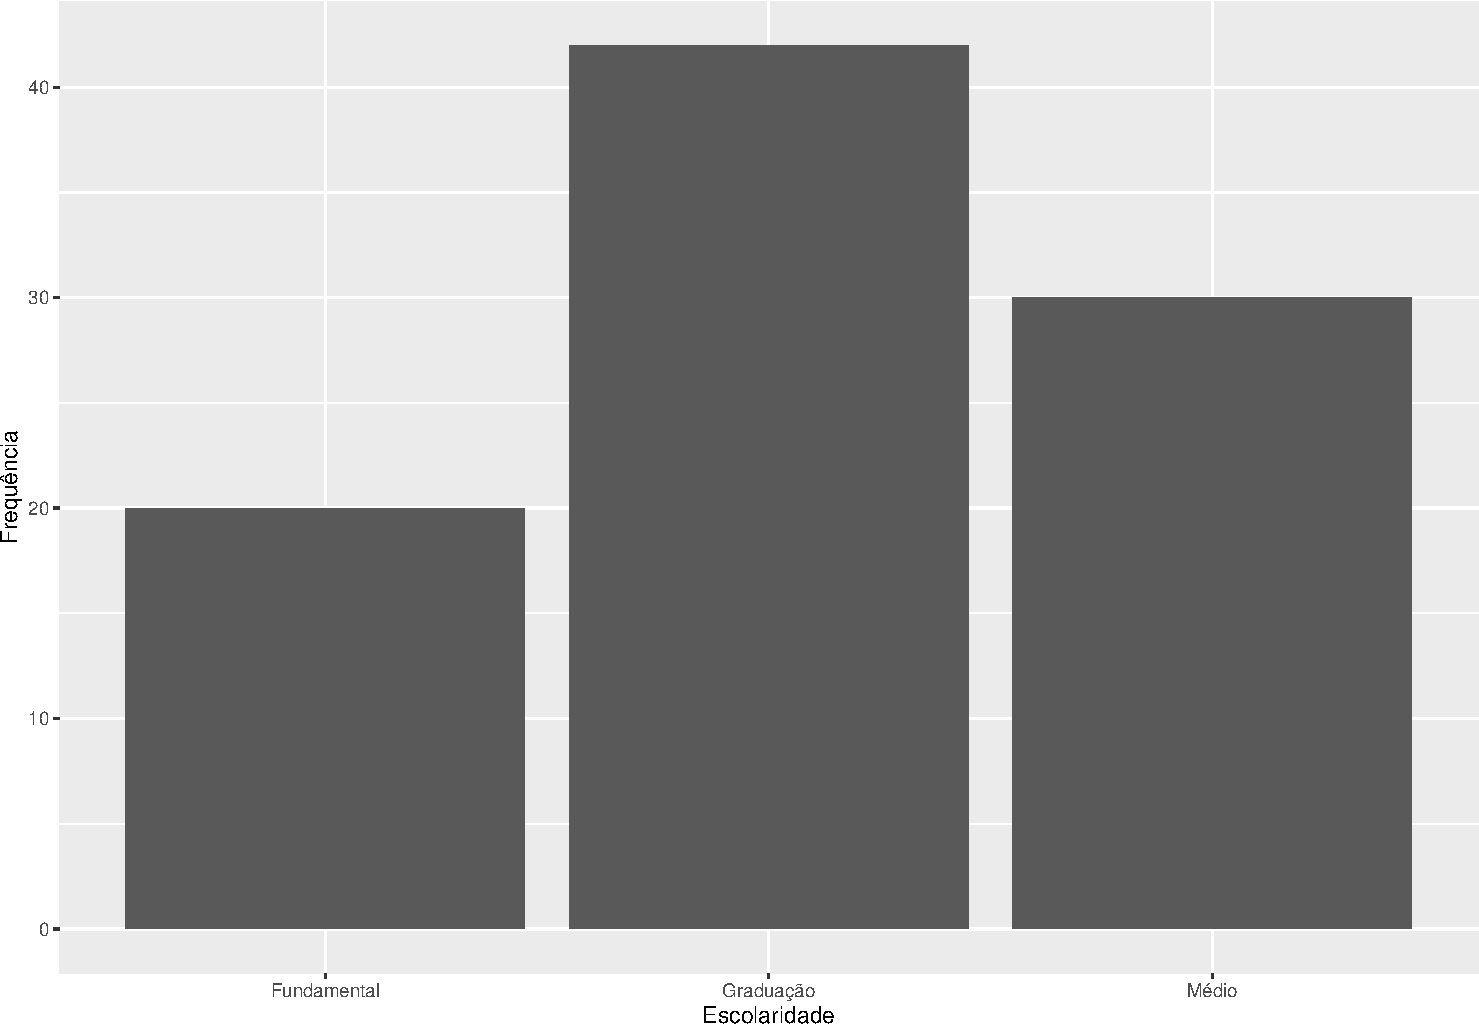
\includegraphics[keepaspectratio]{index_beamer_files/figure-beamer/unnamed-chunk-23-1.pdf}}
\end{block}

\begin{block}{Manipulação da legenda}
\phantomsection\label{manipulauxe7uxe3o-da-legenda}
Caso queremos tirar a legenda ou alterar a posição da legenda,
utilizaremos o argumento \texttt{legend.position\ =}:

\begin{itemize}
\item
  \textbf{``none''} para tirar a legenda
\item
  \textbf{``top''} para a legenda ficar em cima
\item
  \textbf{``bottom''} para a legenda ficar em baixo
\item
  \textbf{``left''} para a legenda ficar na esquerda
\item
  \textbf{``right''} para a legenda ficar na direita
\end{itemize}

\pandocbounded{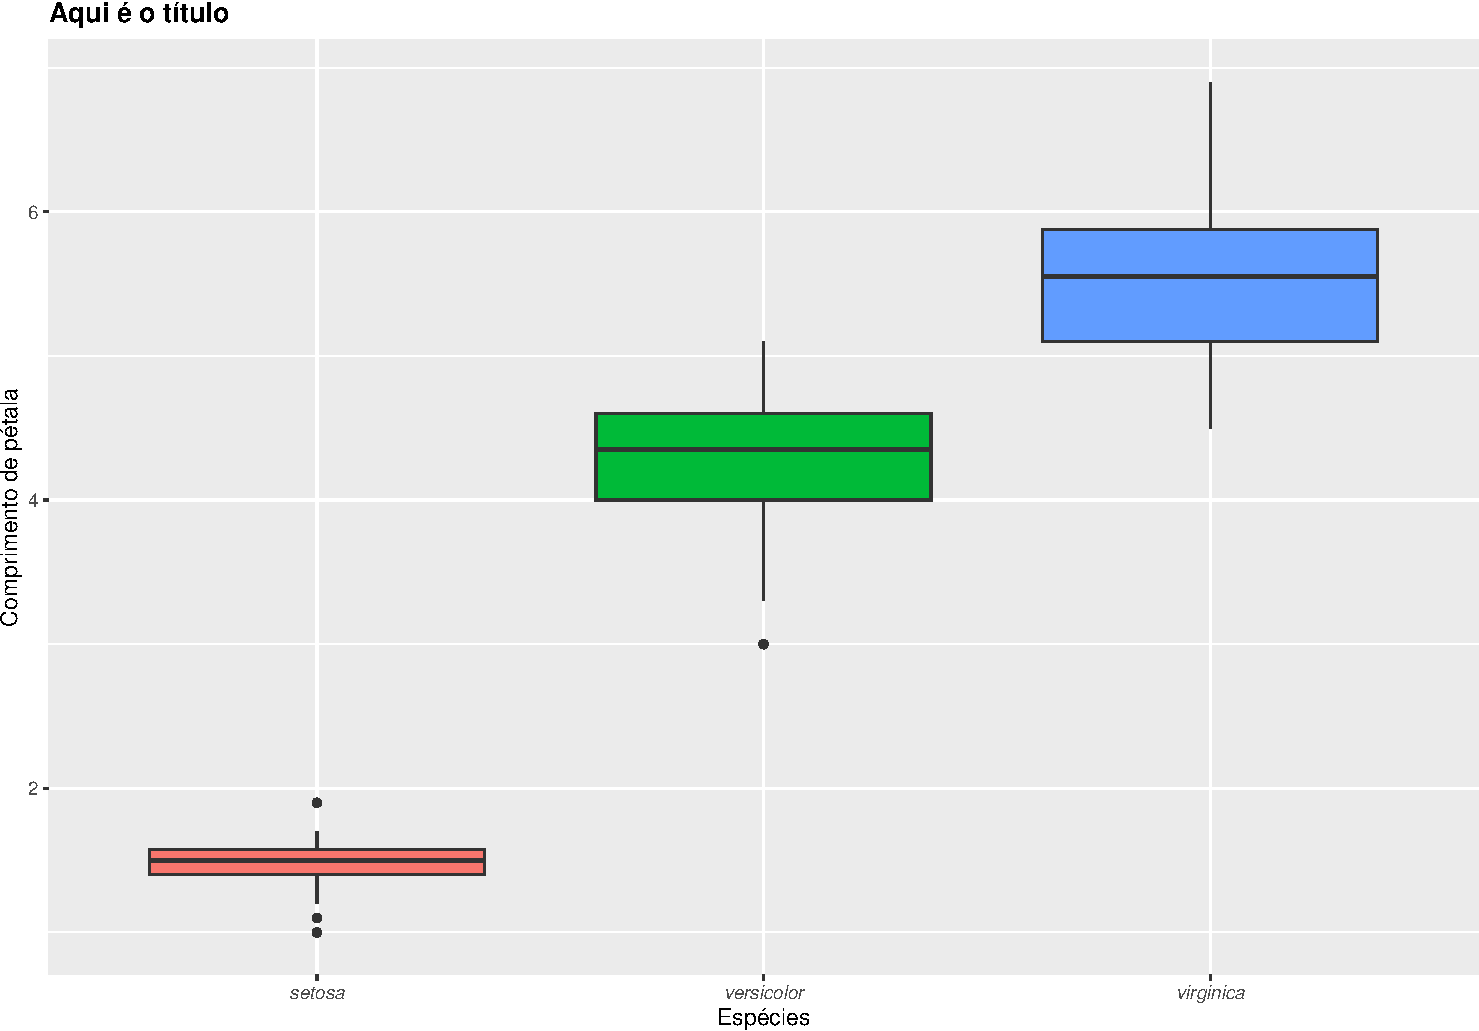
\includegraphics[keepaspectratio]{index_beamer_files/figure-beamer/unnamed-chunk-24-1.pdf}}

\pandocbounded{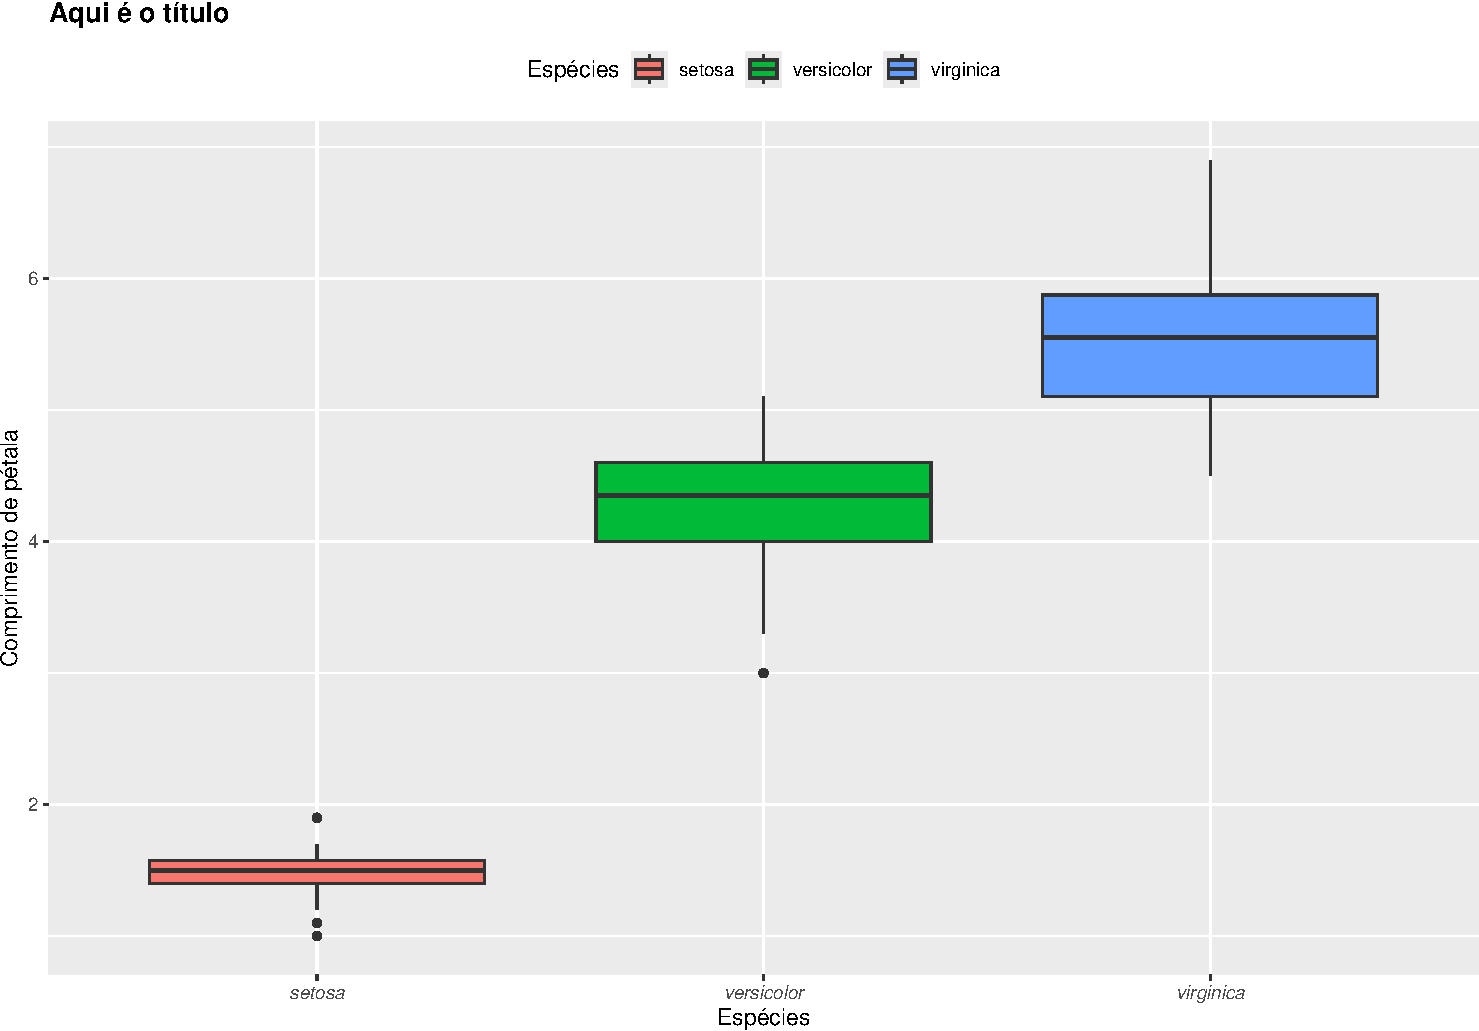
\includegraphics[keepaspectratio]{index_beamer_files/figure-beamer/unnamed-chunk-24-2.pdf}}

\pandocbounded{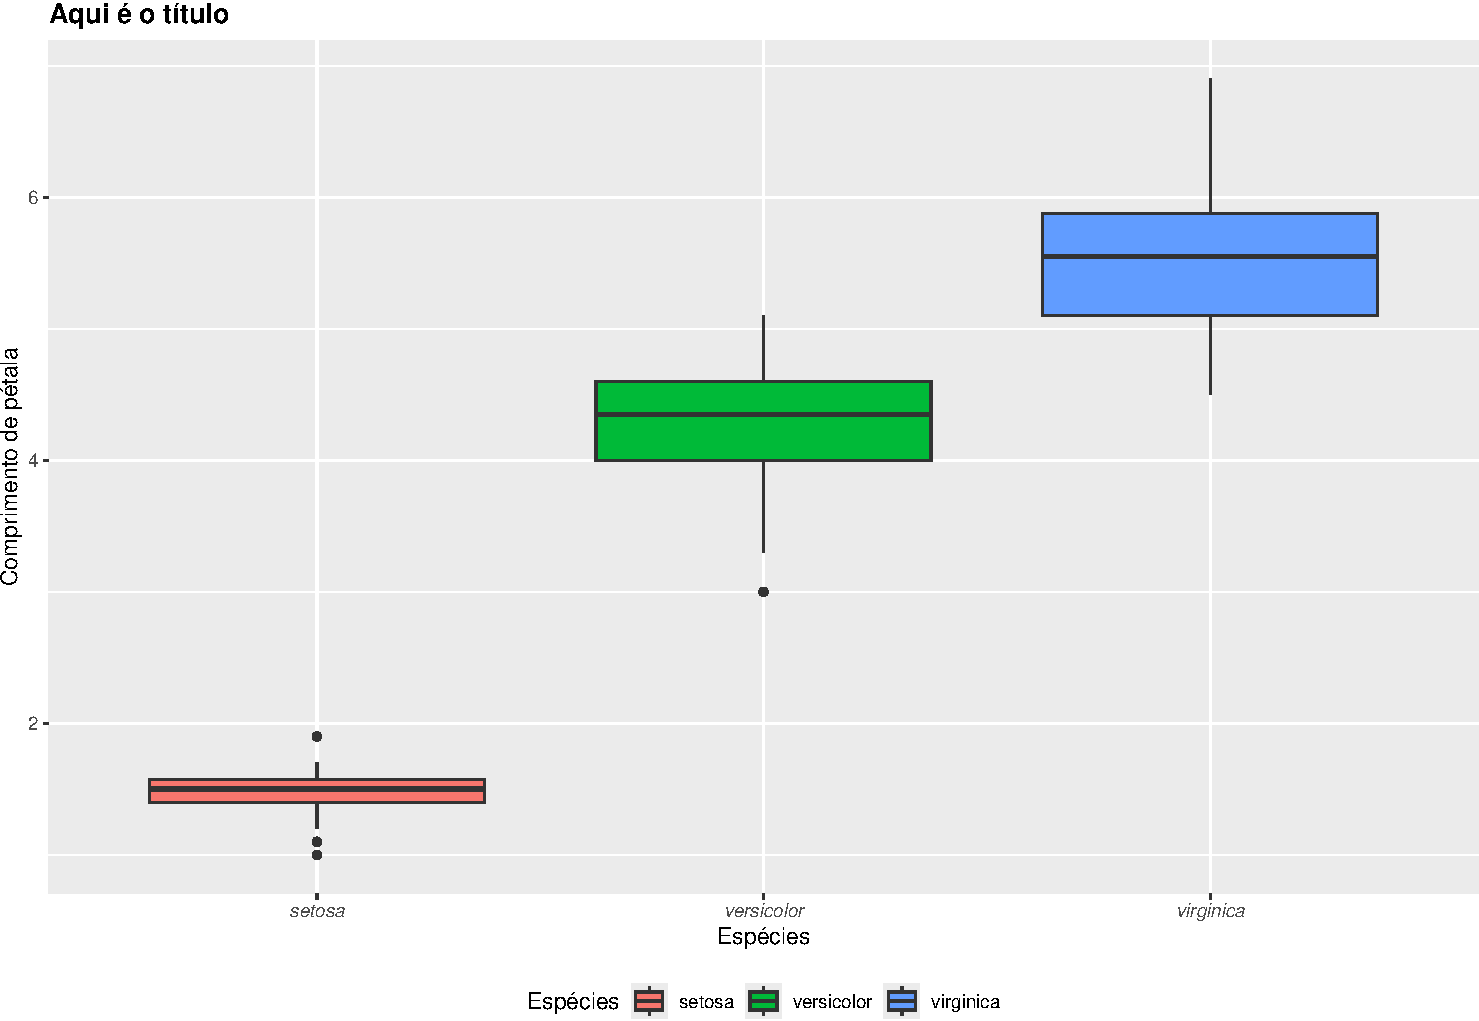
\includegraphics[keepaspectratio]{index_beamer_files/figure-beamer/unnamed-chunk-24-3.pdf}}

\pandocbounded{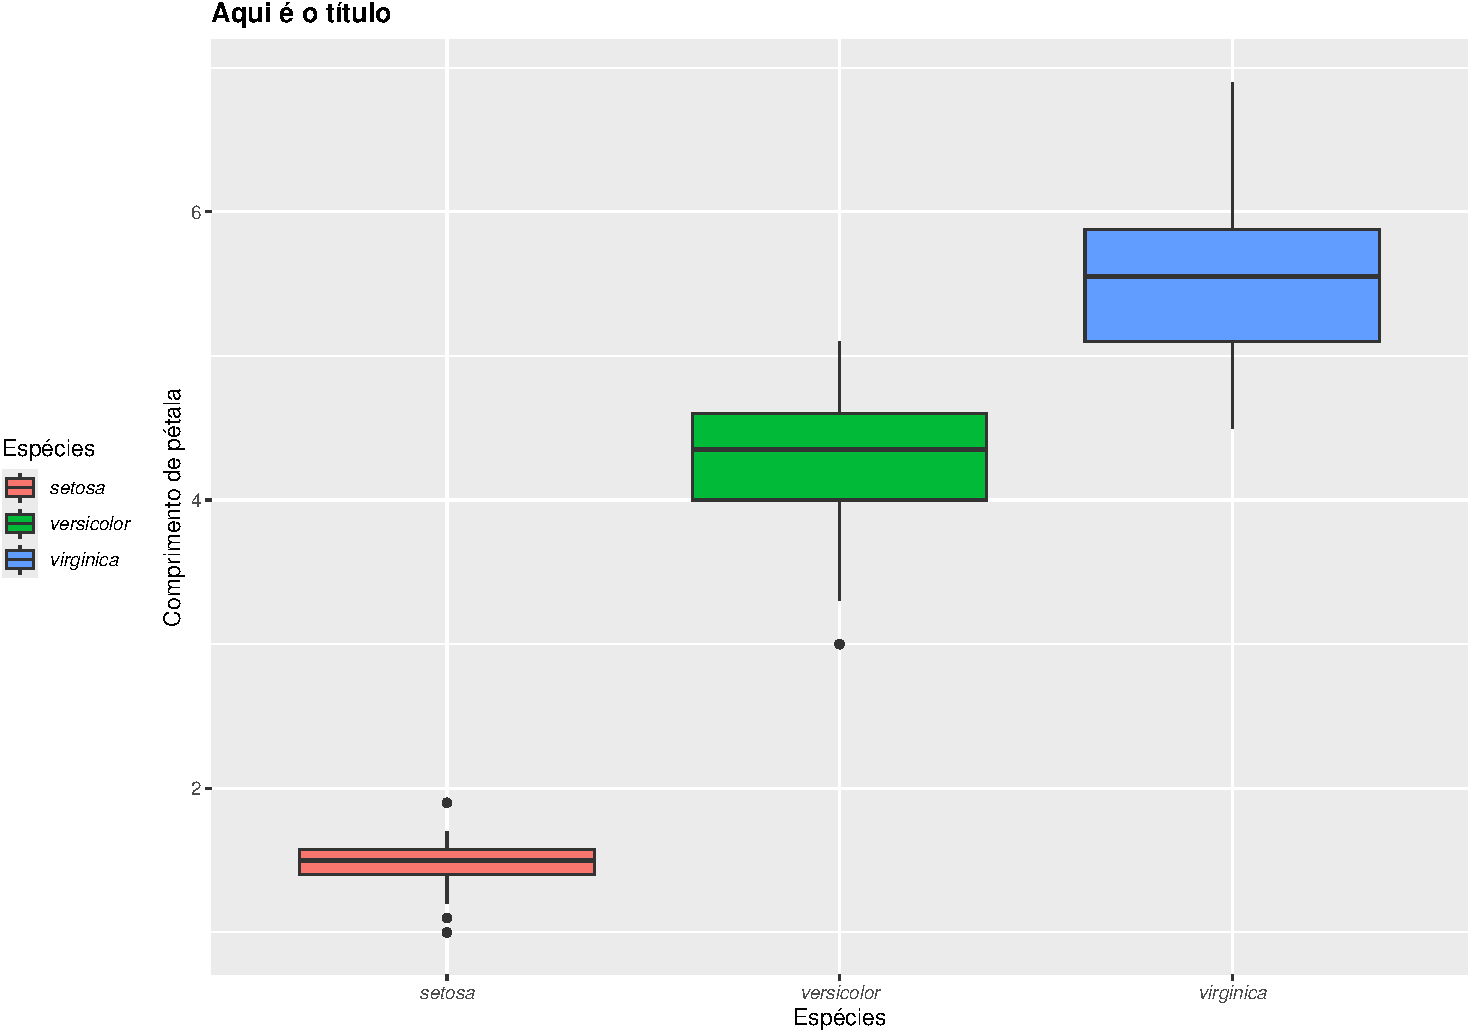
\includegraphics[keepaspectratio]{index_beamer_files/figure-beamer/unnamed-chunk-24-4.pdf}}
\end{block}

\begin{block}{Anotação em gráfico}
\phantomsection\label{anotauxe7uxe3o-em-gruxe1fico}
Também é possível fazer anotações em gráficos no ggplot2, como colocar
linhas e anotações para destacar pontos interessantes.

No primeiro exemplo colocamos o \texttt{geom\_text} para adicionar o
texto. Os argumentos \texttt{x} e \texttt{y} são para delimitar onde vai
ficar o nosso texto, \texttt{label} é para definir o que vai estar no
texto (nunca se esqueça de colocar entre aspas \texttt{"\ "}).

\pandocbounded{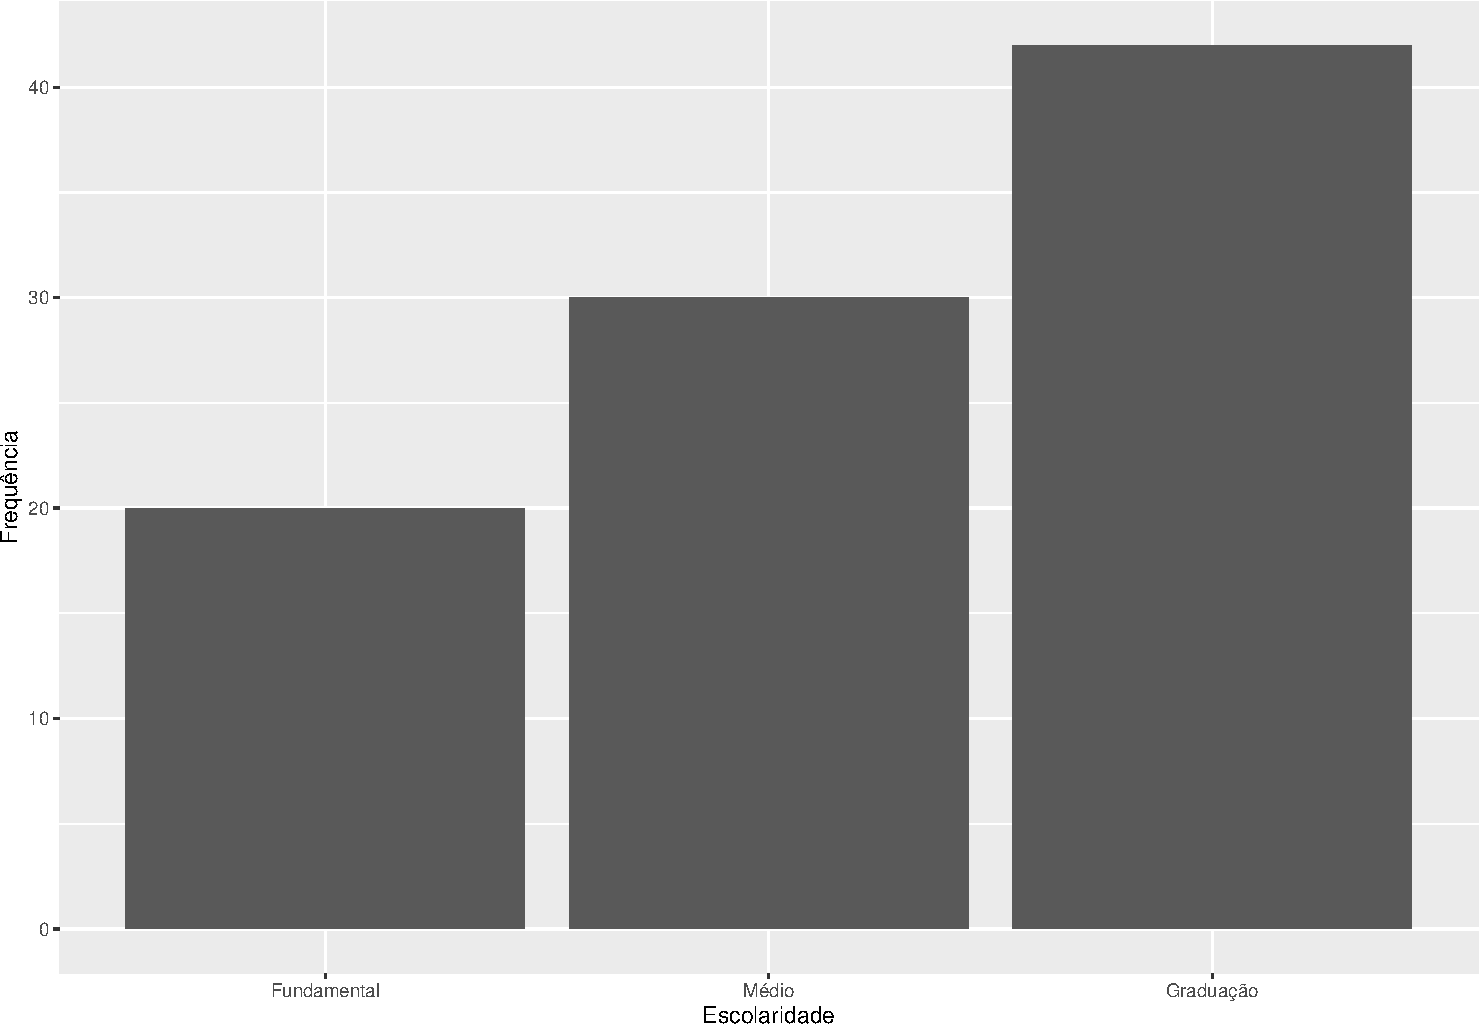
\includegraphics[keepaspectratio]{index_beamer_files/figure-beamer/unnamed-chunk-25-1.pdf}}

Aqui é um exemplo utilizando \texttt{annotate}, nele além de adicionar
texto, você pode adicionar linhas. Como nesse caso colocamos uma linha
vertical no gráfico utilizando o argumento \texttt{"vline"}. Para
colocar uma linha na horizontal é \texttt{"hline"}. Para ser um texto se
utiliza o argumento \texttt{"text"}.

\pandocbounded{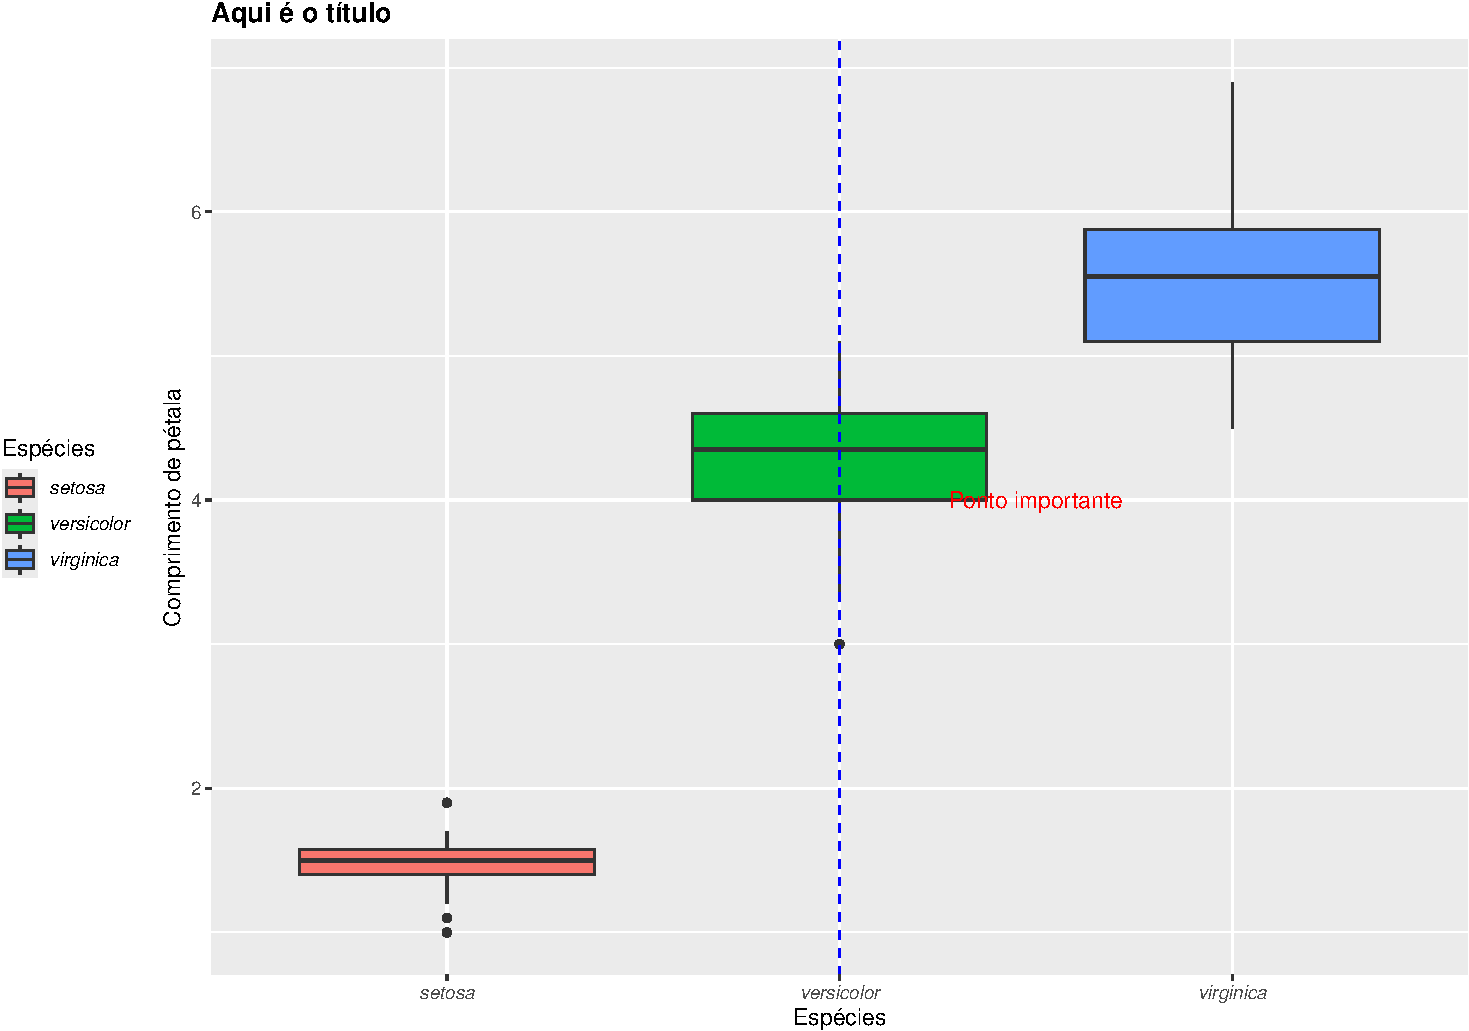
\includegraphics[keepaspectratio]{index_beamer_files/figure-beamer/unnamed-chunk-26-1.pdf}}

\pandocbounded{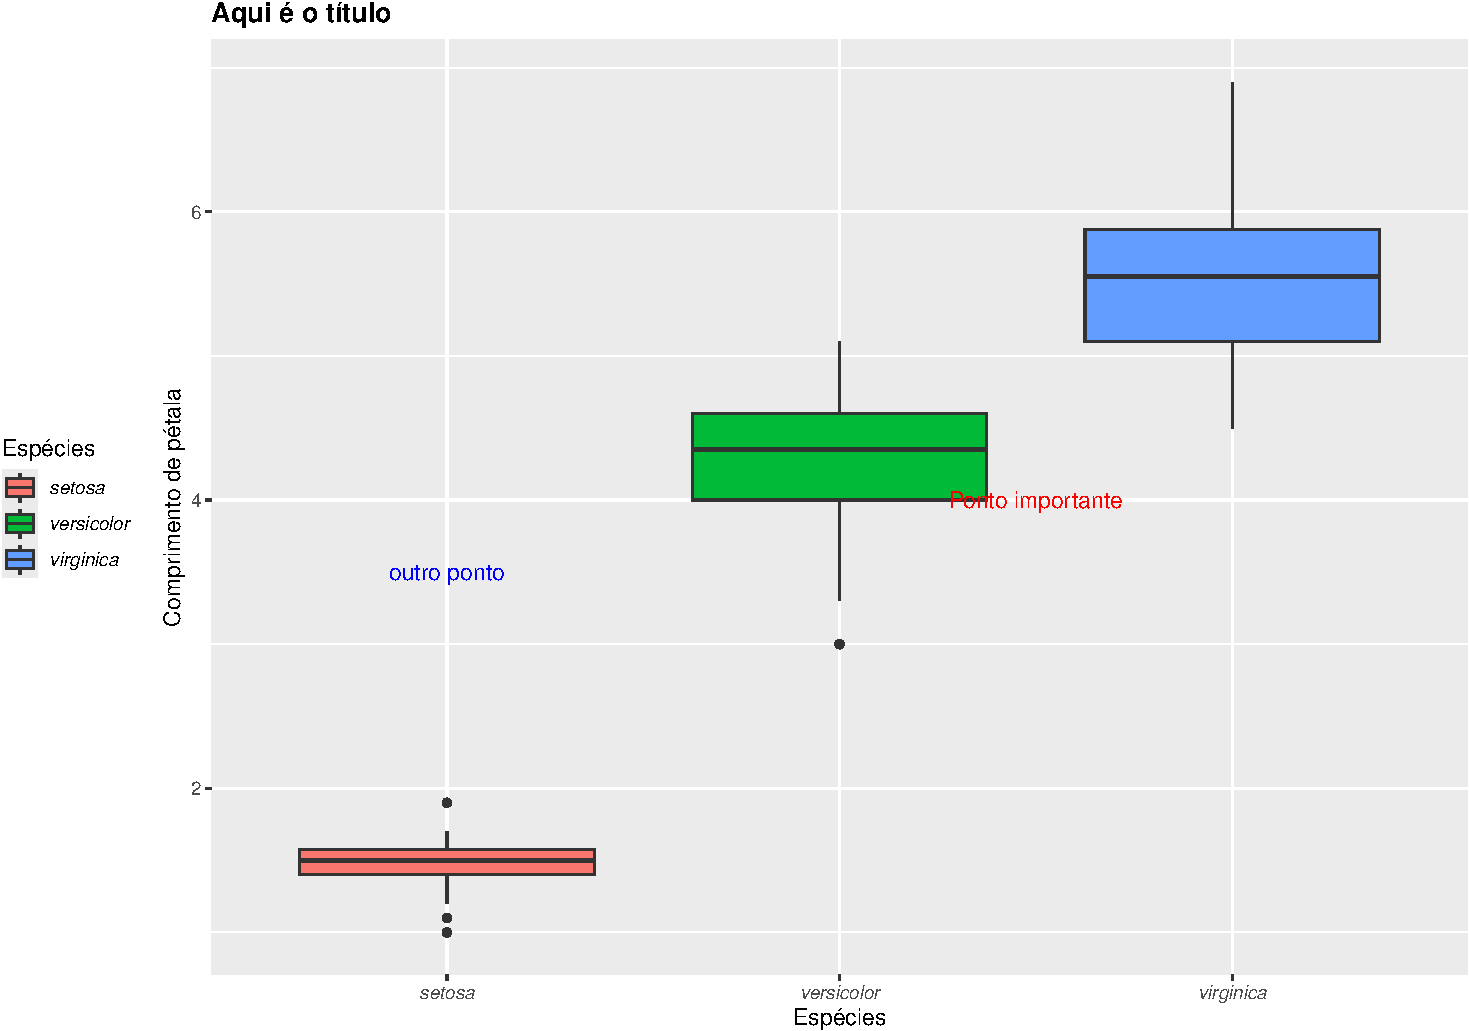
\includegraphics[keepaspectratio]{index_beamer_files/figure-beamer/unnamed-chunk-26-2.pdf}}
\end{block}
\end{frame}

\begin{frame}{Temas (\texttt{theme\_*})}
\phantomsection\label{temas-theme_}
\pandocbounded{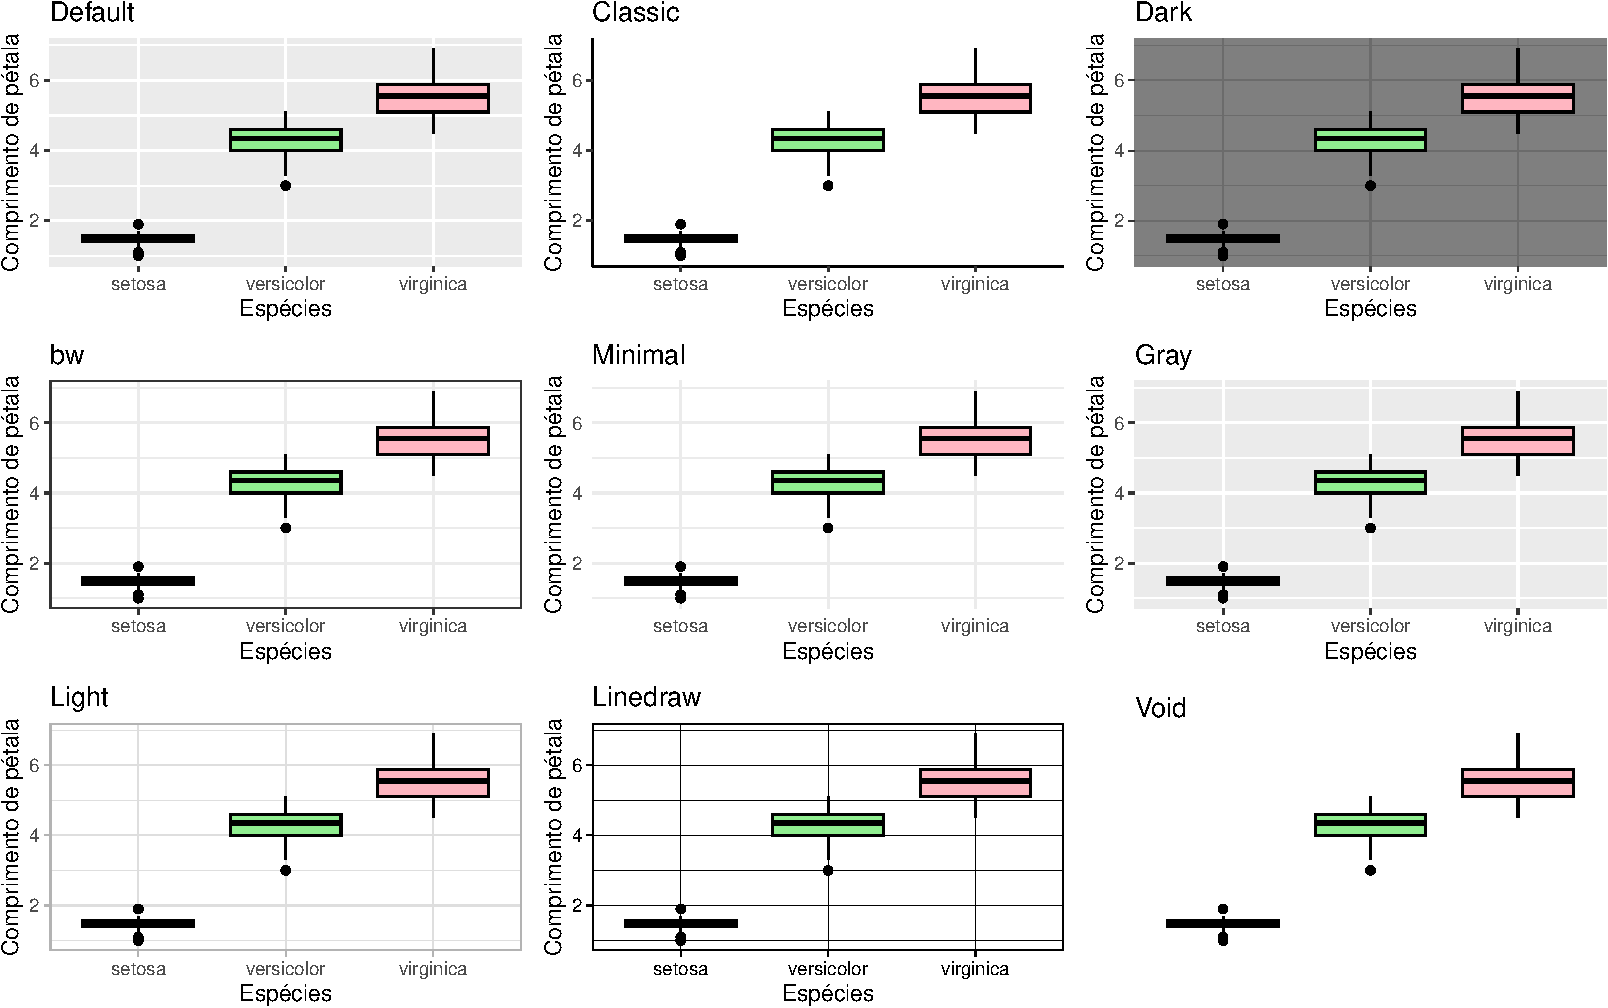
\includegraphics[keepaspectratio]{index_beamer_files/figure-beamer/Box-plot tema-1.pdf}}
\end{frame}

\begin{frame}[fragile]{Unindo vários gráficos em uma imagem só}
\phantomsection\label{unindo-vuxe1rios-gruxe1ficos-em-uma-imagem-suxf3}
\pandocbounded{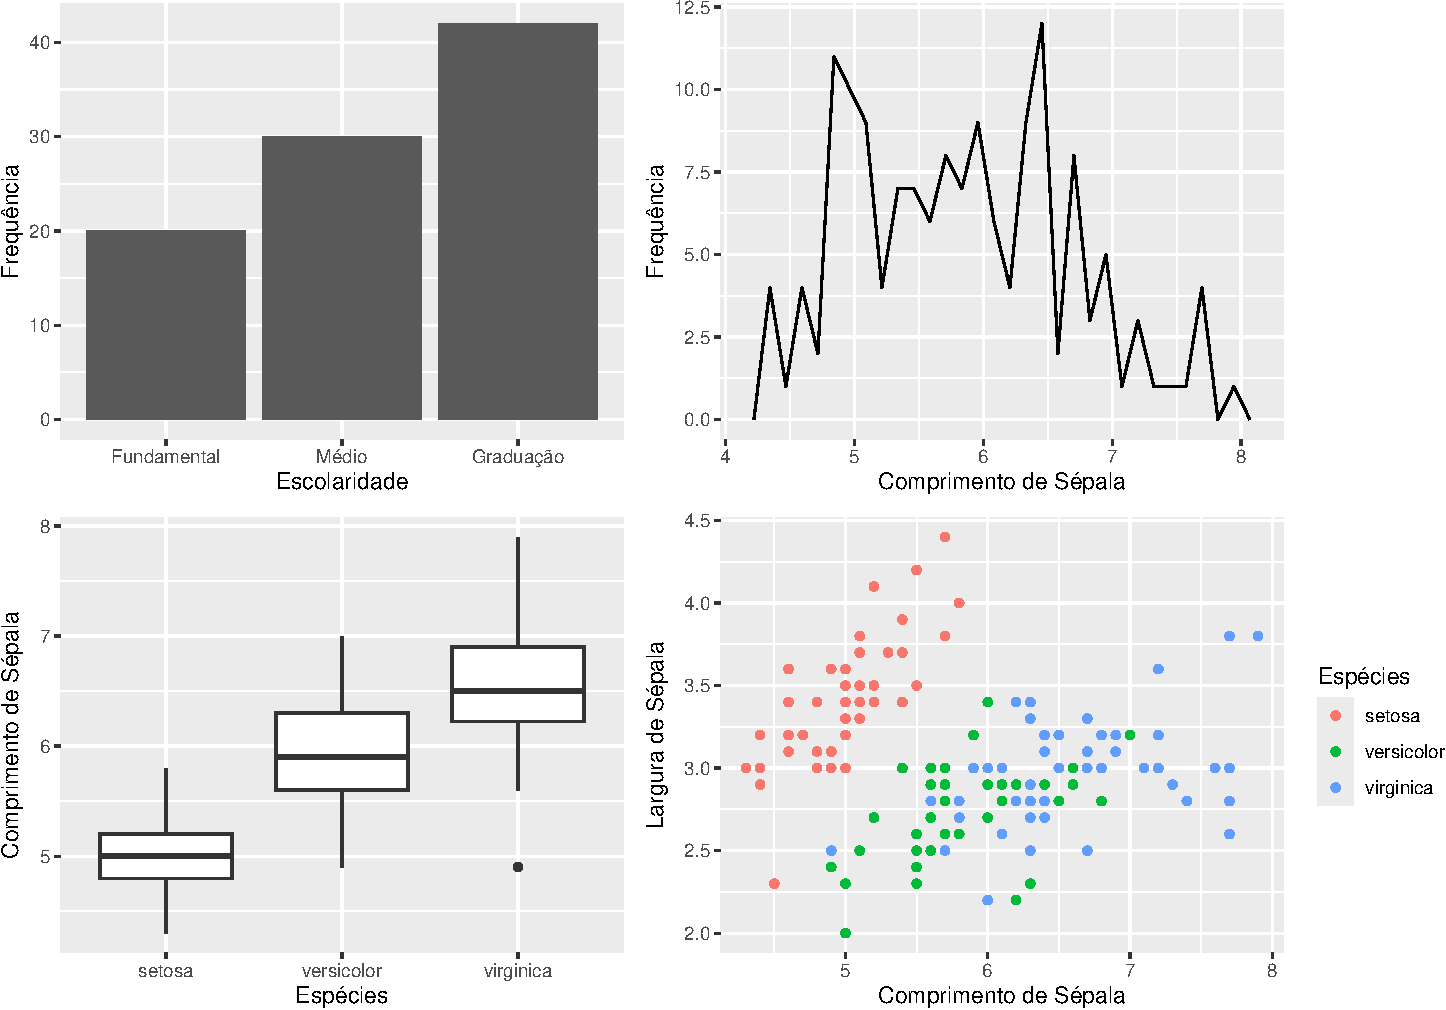
\includegraphics[keepaspectratio]{index_beamer_files/figure-beamer/unnamed-chunk-27-1.pdf}}

\begin{enumerate}
\setcounter{enumi}{2}
\tightlist
\item
  Também é possível utilizar diferêntes conformações utilizando
  elementos matemáticos, como \texttt{/} e \texttt{()}.
\end{enumerate}

\pandocbounded{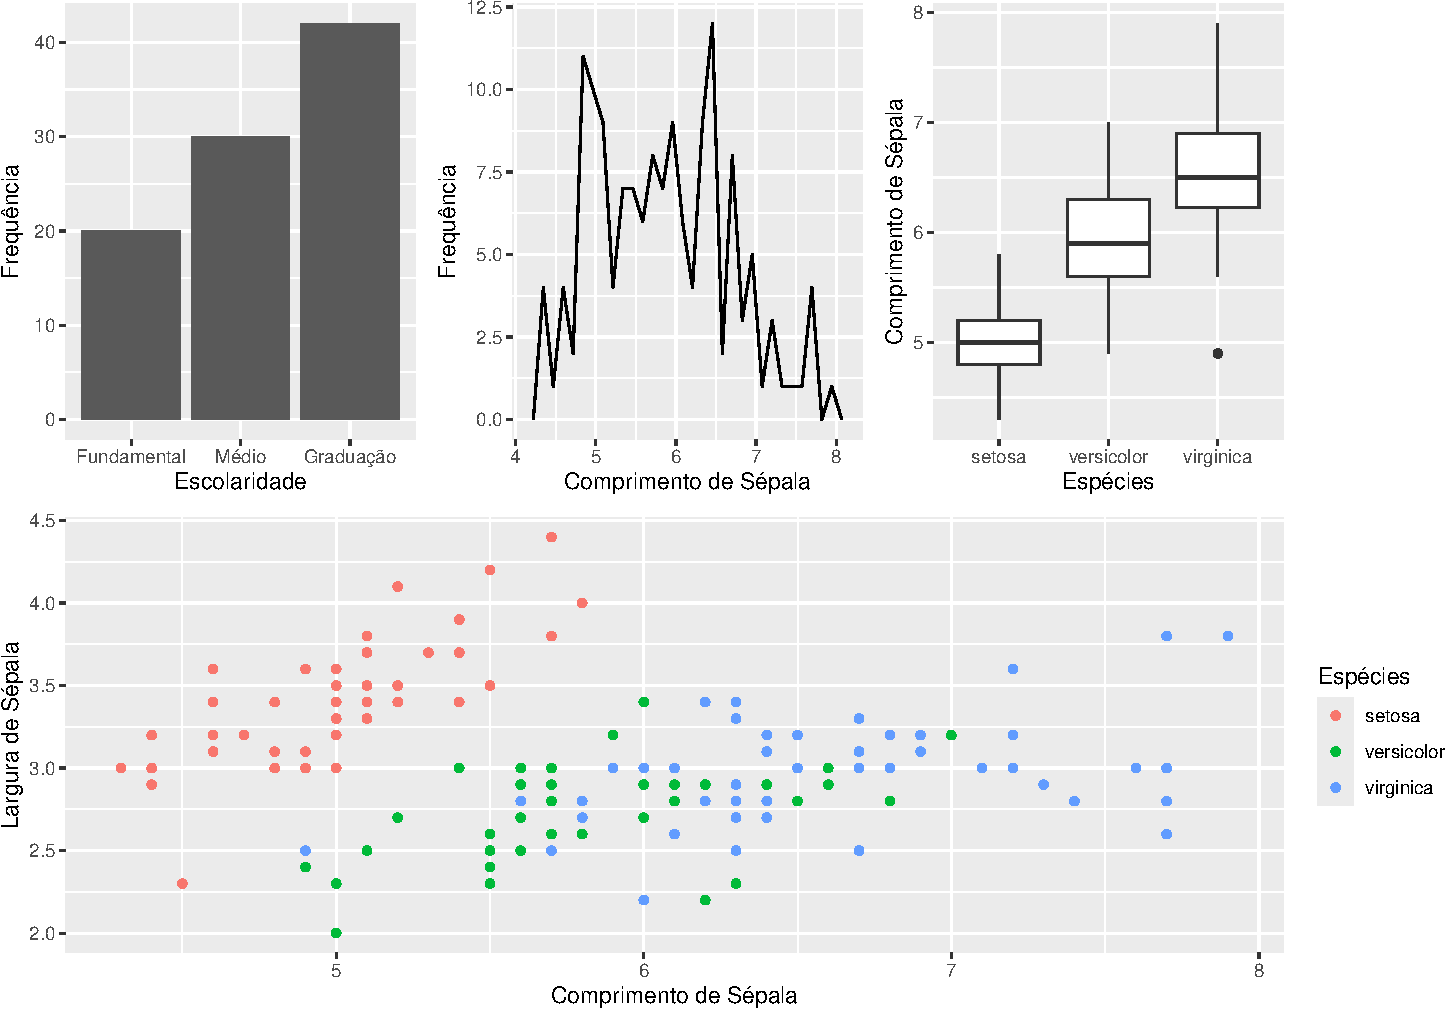
\includegraphics[keepaspectratio]{index_beamer_files/figure-beamer/unnamed-chunk-28-1.pdf}}
\end{frame}

\section{Extra}\label{extra}

\begin{frame}[fragile]{Mapas}
\phantomsection\label{mapas}
\begin{Shaded}
\begin{Highlighting}[]
\CommentTok{\#instalando o pacote raster e sf}
\FunctionTok{install.packages}\NormalTok{(}\StringTok{"raster"}\NormalTok{)}
\FunctionTok{install.packages}\NormalTok{(}\StringTok{"sf"}\NormalTok{)}

\CommentTok{\#carregando o pacote raster e sf}
\FunctionTok{library}\NormalTok{(raster)}
\FunctionTok{library}\NormalTok{(sf)}
\end{Highlighting}
\end{Shaded}
\end{frame}

\begin{frame}[fragile]
\begin{Shaded}
\begin{Highlighting}[]
\CommentTok{\# Importando dados}
\NormalTok{prec}\OtherTok{\textless{}{-}}\FunctionTok{raster}\NormalTok{(}\StringTok{"pelprec.tiff"}\NormalTok{)}

\NormalTok{pel}\OtherTok{\textless{}{-}}\FunctionTok{read\_sf}\NormalTok{(}\StringTok{"Pelotas/Pelotas.shp"}\NormalTok{)}

\CommentTok{\# Convertendo raster para data frame para o ggplot processar o dado}
\NormalTok{prec\_df}\OtherTok{\textless{}{-}}\FunctionTok{as.data.frame}\NormalTok{(prec, }\AttributeTok{xy =} \ConstantTok{TRUE}\NormalTok{, }\AttributeTok{na.rm =} \ConstantTok{TRUE}\NormalTok{)}

\FunctionTok{head}\NormalTok{(prec\_df)}
\end{Highlighting}
\end{Shaded}

\begin{verbatim}
           x         y pelprec
14 -52.49583 -31.32917     120
15 -52.48750 -31.32917     121
16 -52.47917 -31.32917     121
17 -52.47083 -31.32917     120
18 -52.46250 -31.32917     120
19 -52.45417 -31.32917     120
\end{verbatim}
\end{frame}

\begin{frame}[fragile]
\begin{Shaded}
\begin{Highlighting}[]
\FunctionTok{ggplot}\NormalTok{(prec\_df,}\FunctionTok{aes}\NormalTok{(}\AttributeTok{x=}\NormalTok{x,}\AttributeTok{y=}\NormalTok{y,}\AttributeTok{fill=}\NormalTok{pelprec))}\SpecialCharTok{+}\FunctionTok{geom\_raster}\NormalTok{()}
\end{Highlighting}
\end{Shaded}

\pandocbounded{\includegraphics[keepaspectratio]{index_beamer_files/figure-beamer/unnamed-chunk-31-1.pdf}}
\end{frame}

\begin{frame}[fragile]
\begin{Shaded}
\begin{Highlighting}[]
\CommentTok{\# Cores padrão}
\FunctionTok{ggplot}\NormalTok{()}\SpecialCharTok{+}\FunctionTok{geom\_raster}\NormalTok{(}\AttributeTok{data=}\NormalTok{prec\_df,}\FunctionTok{aes}\NormalTok{(}\AttributeTok{x=}\NormalTok{x,}\AttributeTok{y=}\NormalTok{y,}\AttributeTok{fill=}\NormalTok{pelprec))}\SpecialCharTok{+}\FunctionTok{geom\_sf}\NormalTok{(}\AttributeTok{data=}\NormalTok{pel,}\AttributeTok{fill=}\ConstantTok{NA}\NormalTok{, }\AttributeTok{color=}\StringTok{"gray"}\NormalTok{,}\AttributeTok{linewidth=}\DecValTok{2}\NormalTok{, }\AttributeTok{alpha=}\NormalTok{.}\DecValTok{01}\NormalTok{)}\SpecialCharTok{+}\FunctionTok{labs}\NormalTok{(}\AttributeTok{title=}\StringTok{"Mapa da média anual da precipitação }\SpecialCharTok{\textbackslash{}n}\StringTok{ em Pelotas{-}RS entre 1970{-}2000"}\NormalTok{, }\AttributeTok{y=}\StringTok{"Latitude"}\NormalTok{, }\AttributeTok{x=}\StringTok{"Longitude"}\NormalTok{, }\AttributeTok{fill=}\StringTok{"Precipitação (mm)"}\NormalTok{)}\SpecialCharTok{+}\FunctionTok{theme\_bw}\NormalTok{()}
\end{Highlighting}
\end{Shaded}

\pandocbounded{\includegraphics[keepaspectratio]{index_beamer_files/figure-beamer/unnamed-chunk-32-1.pdf}}

\begin{Shaded}
\begin{Highlighting}[]
\FunctionTok{ggplot}\NormalTok{()}\SpecialCharTok{+}\FunctionTok{geom\_raster}\NormalTok{(}\AttributeTok{data=}\NormalTok{prec\_df,}\FunctionTok{aes}\NormalTok{(}\AttributeTok{x=}\NormalTok{x,}\AttributeTok{y=}\NormalTok{y,}\AttributeTok{fill=}\NormalTok{pelprec))}\SpecialCharTok{+}\FunctionTok{geom\_sf}\NormalTok{(}\AttributeTok{data=}\NormalTok{pel,}\AttributeTok{fill=}\ConstantTok{NA}\NormalTok{, }\AttributeTok{color=}\StringTok{"gray"}\NormalTok{,}\AttributeTok{linewidth=}\DecValTok{2}\NormalTok{, }\AttributeTok{alpha=}\NormalTok{.}\DecValTok{01}\NormalTok{)}\SpecialCharTok{+}\FunctionTok{labs}\NormalTok{(}\AttributeTok{title=}\StringTok{"Mapa da média anual da precipitação }\SpecialCharTok{\textbackslash{}n}\StringTok{ em Pelotas{-}RS entre 1970{-}2000"}\NormalTok{, }\AttributeTok{y=}\StringTok{"Latitude"}\NormalTok{, }\AttributeTok{x=}\StringTok{"Longitude"}\NormalTok{, }\AttributeTok{fill=}\StringTok{"Precipitação (mm)"}\NormalTok{)}\SpecialCharTok{+}\FunctionTok{theme\_bw}\NormalTok{()}\SpecialCharTok{+}\FunctionTok{scale\_fill\_gradient}\NormalTok{(}\AttributeTok{low=}\StringTok{"gray"}\NormalTok{,}\AttributeTok{high=}\StringTok{"blue"}\NormalTok{)}
\end{Highlighting}
\end{Shaded}

\pandocbounded{\includegraphics[keepaspectratio]{index_beamer_files/figure-beamer/unnamed-chunk-32-2.pdf}}

\begin{Shaded}
\begin{Highlighting}[]
\FunctionTok{ggplot}\NormalTok{()}\SpecialCharTok{+}\FunctionTok{geom\_raster}\NormalTok{(}\AttributeTok{data=}\NormalTok{prec\_df,}\FunctionTok{aes}\NormalTok{(}\AttributeTok{x=}\NormalTok{x,}\AttributeTok{y=}\NormalTok{y,}\AttributeTok{fill=}\NormalTok{pelprec))}\SpecialCharTok{+}\FunctionTok{geom\_sf}\NormalTok{(}\AttributeTok{data=}\NormalTok{pel,}\AttributeTok{fill=}\ConstantTok{NA}\NormalTok{, }\AttributeTok{color=}\StringTok{"gray"}\NormalTok{,}\AttributeTok{linewidth=}\DecValTok{2}\NormalTok{, }\AttributeTok{alpha=}\NormalTok{.}\DecValTok{01}\NormalTok{)}\SpecialCharTok{+}\FunctionTok{labs}\NormalTok{(}\AttributeTok{title=}\StringTok{"Mapa da média anual da precipitação }\SpecialCharTok{\textbackslash{}n}\StringTok{ em Pelotas{-}RS entre 1970{-}2000"}\NormalTok{, }\AttributeTok{y=}\StringTok{"Latitude"}\NormalTok{, }\AttributeTok{x=}\StringTok{"Longitude"}\NormalTok{, }\AttributeTok{fill=}\StringTok{"Precipitação (mm)"}\NormalTok{)}\SpecialCharTok{+}\FunctionTok{theme\_bw}\NormalTok{()}\SpecialCharTok{+}\FunctionTok{scale\_fill\_gradientn}\NormalTok{(}\AttributeTok{colours =} \FunctionTok{terrain.colors}\NormalTok{(}\DecValTok{10}\NormalTok{))}
\end{Highlighting}
\end{Shaded}

\pandocbounded{\includegraphics[keepaspectratio]{index_beamer_files/figure-beamer/unnamed-chunk-32-3.pdf}}
\end{frame}

\begin{frame}[fragile]
\begin{Shaded}
\begin{Highlighting}[]
\CommentTok{\#intalando pacote viridis}
\FunctionTok{install.packages}\NormalTok{(}\StringTok{"viridis"}\NormalTok{)}
\CommentTok{\#carregando pacote viridis}
\FunctionTok{library}\NormalTok{(viridis)}
\end{Highlighting}
\end{Shaded}
\end{frame}

\begin{frame}
\pandocbounded{\includegraphics[keepaspectratio]{index_beamer_files/figure-beamer/unnamed-chunk-34-1.pdf}}
\end{frame}

\begin{frame}[fragile]{Temas divertidos}
\phantomsection\label{temas-divertidos}
\begin{Shaded}
\begin{Highlighting}[]
\FunctionTok{install.packages}\NormalTok{(}\StringTok{"remotes"}\NormalTok{)}
\NormalTok{remotes}\SpecialCharTok{::}\FunctionTok{install\_github}\NormalTok{(}\StringTok{"MatthewBJane/ThemePark"}\NormalTok{)}
\FunctionTok{library}\NormalTok{(ThemePark)}
\end{Highlighting}
\end{Shaded}
\end{frame}

\begin{frame}[fragile]
\begin{Shaded}
\begin{Highlighting}[]
\NormalTok{iris}\SpecialCharTok{\%\textgreater{}\%}\FunctionTok{ggplot}\NormalTok{(}\FunctionTok{aes}\NormalTok{(}\AttributeTok{x=}\NormalTok{Species, }\AttributeTok{y=}\NormalTok{Petal.Length, }\AttributeTok{fill=}\NormalTok{Species))}\SpecialCharTok{+}\FunctionTok{geom\_boxplot}\NormalTok{(}\AttributeTok{fill=}\FunctionTok{c}\NormalTok{(lordoftherings\_theme\_colors[}\StringTok{"light"}\NormalTok{],lordoftherings\_theme\_colors[}\StringTok{"medium"}\NormalTok{],lordoftherings\_theme\_colors[}\StringTok{"dark"}\NormalTok{]))}\SpecialCharTok{+}\FunctionTok{labs}\NormalTok{(}\AttributeTok{y=}\StringTok{"Comprimento de pétala"}\NormalTok{, }\AttributeTok{x=}\StringTok{"Espécies"}\NormalTok{, }\AttributeTok{title=} \StringTok{"Tema Senhor dos Anéis"}\NormalTok{)}\SpecialCharTok{+}\FunctionTok{theme\_lordoftherings}\NormalTok{()}
\end{Highlighting}
\end{Shaded}

\pandocbounded{\includegraphics[keepaspectratio]{index_beamer_files/figure-beamer/theme park-1.pdf}}

\begin{Shaded}
\begin{Highlighting}[]
\NormalTok{iris}\SpecialCharTok{\%\textgreater{}\%}\FunctionTok{ggplot}\NormalTok{(}\FunctionTok{aes}\NormalTok{(}\AttributeTok{x=}\NormalTok{Species, }\AttributeTok{y=}\NormalTok{Petal.Length, }\AttributeTok{fill=}\NormalTok{Species))}\SpecialCharTok{+}\FunctionTok{geom\_boxplot}\NormalTok{(}\AttributeTok{fill=}\FunctionTok{c}\NormalTok{(barbie\_theme\_colors[}\StringTok{"light"}\NormalTok{],barbie\_theme\_colors[}\StringTok{"medium"}\NormalTok{],barbie\_theme\_colors[}\StringTok{"dark"}\NormalTok{]))}\SpecialCharTok{+}\FunctionTok{labs}\NormalTok{(}\AttributeTok{y=}\StringTok{"Comprimento de pétala"}\NormalTok{, }\AttributeTok{x=}\StringTok{"Espécies"}\NormalTok{, }\AttributeTok{title=} \StringTok{"Tema Barbie"}\NormalTok{)}\SpecialCharTok{+}\FunctionTok{theme\_barbie}\NormalTok{()}
\end{Highlighting}
\end{Shaded}

\pandocbounded{\includegraphics[keepaspectratio]{index_beamer_files/figure-beamer/theme park-2.pdf}}

\begin{Shaded}
\begin{Highlighting}[]
\NormalTok{iris}\SpecialCharTok{\%\textgreater{}\%}\FunctionTok{ggplot}\NormalTok{(}\FunctionTok{aes}\NormalTok{(}\AttributeTok{x=}\NormalTok{Species, }\AttributeTok{y=}\NormalTok{Petal.Length, }\AttributeTok{fill=}\NormalTok{Species))}\SpecialCharTok{+}\FunctionTok{geom\_boxplot}\NormalTok{(}\AttributeTok{fill=}\FunctionTok{c}\NormalTok{(simpsons\_theme\_colors[}\StringTok{"light"}\NormalTok{],simpsons\_theme\_colors[}\StringTok{"medium"}\NormalTok{],simpsons\_theme\_colors[}\StringTok{"dark"}\NormalTok{]))}\SpecialCharTok{+}\FunctionTok{labs}\NormalTok{(}\AttributeTok{y=}\StringTok{"Comprimento de pétala"}\NormalTok{, }\AttributeTok{x=}\StringTok{"Espécies"}\NormalTok{, }\AttributeTok{title=} \StringTok{"Tema Simpsons"}\NormalTok{)}\SpecialCharTok{+}\FunctionTok{theme\_simpsons}\NormalTok{()}
\end{Highlighting}
\end{Shaded}

\pandocbounded{\includegraphics[keepaspectratio]{index_beamer_files/figure-beamer/theme park-3.pdf}}

\begin{Shaded}
\begin{Highlighting}[]
\NormalTok{iris}\SpecialCharTok{\%\textgreater{}\%}\FunctionTok{ggplot}\NormalTok{(}\FunctionTok{aes}\NormalTok{(}\AttributeTok{x=}\NormalTok{Species, }\AttributeTok{y=}\NormalTok{Petal.Length, }\AttributeTok{fill=}\NormalTok{Species))}\SpecialCharTok{+}\FunctionTok{geom\_boxplot}\NormalTok{(}\AttributeTok{fill=}\FunctionTok{c}\NormalTok{(friends\_theme\_colors[}\StringTok{"light"}\NormalTok{],friends\_theme\_colors[}\StringTok{"medium"}\NormalTok{],friends\_theme\_colors[}\StringTok{"dark"}\NormalTok{]))}\SpecialCharTok{+}\FunctionTok{labs}\NormalTok{(}\AttributeTok{y=}\StringTok{"Comprimento de pétala"}\NormalTok{, }\AttributeTok{x=}\StringTok{"Espécies"}\NormalTok{, }\AttributeTok{title=} \StringTok{"Tema Friends"}\NormalTok{)}\SpecialCharTok{+}\FunctionTok{theme\_friends}\NormalTok{()}
\end{Highlighting}
\end{Shaded}

\pandocbounded{\includegraphics[keepaspectratio]{index_beamer_files/figure-beamer/theme park-4.pdf}}

\begin{Shaded}
\begin{Highlighting}[]
\NormalTok{iris}\SpecialCharTok{\%\textgreater{}\%}\FunctionTok{ggplot}\NormalTok{(}\FunctionTok{aes}\NormalTok{(}\AttributeTok{x=}\NormalTok{Species, }\AttributeTok{y=}\NormalTok{Petal.Length, }\AttributeTok{fill=}\NormalTok{Species))}\SpecialCharTok{+}\FunctionTok{geom\_boxplot}\NormalTok{(}\AttributeTok{fill=}\FunctionTok{c}\NormalTok{(starwars\_theme\_colors[}\StringTok{"light"}\NormalTok{],starwars\_theme\_colors[}\StringTok{"medium"}\NormalTok{],starwars\_theme\_colors[}\StringTok{"dark"}\NormalTok{]))}\SpecialCharTok{+}\FunctionTok{labs}\NormalTok{(}\AttributeTok{y=}\StringTok{"Comprimento de pétala"}\NormalTok{, }\AttributeTok{x=}\StringTok{"Espécies"}\NormalTok{, }\AttributeTok{title=} \StringTok{"Tema Star wars"}\NormalTok{)}\SpecialCharTok{+}\FunctionTok{theme\_starwars}\NormalTok{()}
\end{Highlighting}
\end{Shaded}

\pandocbounded{\includegraphics[keepaspectratio]{index_beamer_files/figure-beamer/theme park-5.pdf}}
\end{frame}

\begin{frame}{Referências}
\phantomsection\label{referuxeancias}
\phantomsection\label{refs}
\begin{CSLReferences}{1}{0}
\bibitem[\citeproctext]{ref-plotly}
Sievert, Carson. 2020. \emph{Interactive Web-Based Data Visualization
with r, Plotly, and Shiny}. Chapman; Hall/CRC.
\url{https://plotly-r.com}.

\bibitem[\citeproctext]{ref-ggplot2}
Wickham, Hadley. 2016. \emph{Ggplot2: Elegant Graphics for Data
Analysis}. Springer-Verlag New York.
\url{https://ggplot2.tidyverse.org}.

\bibitem[\citeproctext]{ref-forcats}
---------. 2023. \emph{Forcats: Tools for Working with Categorical
Variables (Factors)}. \url{https://forcats.tidyverse.org/}.

\bibitem[\citeproctext]{ref-dplyr}
Wickham, Hadley, Romain François, Lionel Henry, Kirill Müller, and Davis
Vaughan. 2023. \emph{Dplyr: A Grammar of Data Manipulation}.
\url{https://dplyr.tidyverse.org}.

\bibitem[\citeproctext]{ref-wilkinson2011grammar}
Wilkinson, Leland. 2011. {``The Grammar of Graphics.''} In
\emph{Handbook of Computational Statistics: Concepts and Methods},
375--414. Springer.

\end{CSLReferences}
\end{frame}




\end{document}
